\documentclass[12pt,]{book}
\usepackage{lmodern}
\usepackage{amssymb,amsmath}
\usepackage{ifxetex,ifluatex}
\usepackage{fixltx2e} % provides \textsubscript
\ifnum 0\ifxetex 1\fi\ifluatex 1\fi=0 % if pdftex
  \usepackage[T1]{fontenc}
  \usepackage[utf8]{inputenc}
\else % if luatex or xelatex
  \ifxetex
    \usepackage{mathspec}
  \else
    \usepackage{fontspec}
  \fi
  \defaultfontfeatures{Ligatures=TeX,Scale=MatchLowercase}
    \setmonofont[Mapping=tex-ansi,Scale=0.7]{Source Code Pro}
\fi
% use upquote if available, for straight quotes in verbatim environments
\IfFileExists{upquote.sty}{\usepackage{upquote}}{}
% use microtype if available
\IfFileExists{microtype.sty}{%
\usepackage{microtype}
\UseMicrotypeSet[protrusion]{basicmath} % disable protrusion for tt fonts
}{}
\usepackage[margin=1in]{geometry}
\usepackage{hyperref}
\PassOptionsToPackage{usenames,dvipsnames}{color} % color is loaded by hyperref
\hypersetup{unicode=true,
            pdftitle={Econometrics Notes},
            pdfauthor={Matteo Courthoud},
            colorlinks=true,
            linkcolor=Maroon,
            citecolor=Blue,
            urlcolor=Blue,
            breaklinks=true}
\urlstyle{same}  % don't use monospace font for urls
\usepackage{natbib}
\bibliographystyle{apalike}
\usepackage{color}
\usepackage{fancyvrb}
\newcommand{\VerbBar}{|}
\newcommand{\VERB}{\Verb[commandchars=\\\{\}]}
\DefineVerbatimEnvironment{Highlighting}{Verbatim}{commandchars=\\\{\}}
% Add ',fontsize=\small' for more characters per line
\usepackage{framed}
\definecolor{shadecolor}{RGB}{248,248,248}
\newenvironment{Shaded}{\begin{snugshade}}{\end{snugshade}}
\newcommand{\AlertTok}[1]{\textcolor[rgb]{0.94,0.16,0.16}{#1}}
\newcommand{\AnnotationTok}[1]{\textcolor[rgb]{0.56,0.35,0.01}{\textbf{\textit{#1}}}}
\newcommand{\AttributeTok}[1]{\textcolor[rgb]{0.77,0.63,0.00}{#1}}
\newcommand{\BaseNTok}[1]{\textcolor[rgb]{0.00,0.00,0.81}{#1}}
\newcommand{\BuiltInTok}[1]{#1}
\newcommand{\CharTok}[1]{\textcolor[rgb]{0.31,0.60,0.02}{#1}}
\newcommand{\CommentTok}[1]{\textcolor[rgb]{0.56,0.35,0.01}{\textit{#1}}}
\newcommand{\CommentVarTok}[1]{\textcolor[rgb]{0.56,0.35,0.01}{\textbf{\textit{#1}}}}
\newcommand{\ConstantTok}[1]{\textcolor[rgb]{0.00,0.00,0.00}{#1}}
\newcommand{\ControlFlowTok}[1]{\textcolor[rgb]{0.13,0.29,0.53}{\textbf{#1}}}
\newcommand{\DataTypeTok}[1]{\textcolor[rgb]{0.13,0.29,0.53}{#1}}
\newcommand{\DecValTok}[1]{\textcolor[rgb]{0.00,0.00,0.81}{#1}}
\newcommand{\DocumentationTok}[1]{\textcolor[rgb]{0.56,0.35,0.01}{\textbf{\textit{#1}}}}
\newcommand{\ErrorTok}[1]{\textcolor[rgb]{0.64,0.00,0.00}{\textbf{#1}}}
\newcommand{\ExtensionTok}[1]{#1}
\newcommand{\FloatTok}[1]{\textcolor[rgb]{0.00,0.00,0.81}{#1}}
\newcommand{\FunctionTok}[1]{\textcolor[rgb]{0.00,0.00,0.00}{#1}}
\newcommand{\ImportTok}[1]{#1}
\newcommand{\InformationTok}[1]{\textcolor[rgb]{0.56,0.35,0.01}{\textbf{\textit{#1}}}}
\newcommand{\KeywordTok}[1]{\textcolor[rgb]{0.13,0.29,0.53}{\textbf{#1}}}
\newcommand{\NormalTok}[1]{#1}
\newcommand{\OperatorTok}[1]{\textcolor[rgb]{0.81,0.36,0.00}{\textbf{#1}}}
\newcommand{\OtherTok}[1]{\textcolor[rgb]{0.56,0.35,0.01}{#1}}
\newcommand{\PreprocessorTok}[1]{\textcolor[rgb]{0.56,0.35,0.01}{\textit{#1}}}
\newcommand{\RegionMarkerTok}[1]{#1}
\newcommand{\SpecialCharTok}[1]{\textcolor[rgb]{0.00,0.00,0.00}{#1}}
\newcommand{\SpecialStringTok}[1]{\textcolor[rgb]{0.31,0.60,0.02}{#1}}
\newcommand{\StringTok}[1]{\textcolor[rgb]{0.31,0.60,0.02}{#1}}
\newcommand{\VariableTok}[1]{\textcolor[rgb]{0.00,0.00,0.00}{#1}}
\newcommand{\VerbatimStringTok}[1]{\textcolor[rgb]{0.31,0.60,0.02}{#1}}
\newcommand{\WarningTok}[1]{\textcolor[rgb]{0.56,0.35,0.01}{\textbf{\textit{#1}}}}
\usepackage{longtable,booktabs}
\usepackage{graphicx,grffile}
\makeatletter
\def\maxwidth{\ifdim\Gin@nat@width>\linewidth\linewidth\else\Gin@nat@width\fi}
\def\maxheight{\ifdim\Gin@nat@height>\textheight\textheight\else\Gin@nat@height\fi}
\makeatother
% Scale images if necessary, so that they will not overflow the page
% margins by default, and it is still possible to overwrite the defaults
% using explicit options in \includegraphics[width, height, ...]{}
\setkeys{Gin}{width=\maxwidth,height=\maxheight,keepaspectratio}
\IfFileExists{parskip.sty}{%
\usepackage{parskip}
}{% else
\setlength{\parindent}{0pt}
\setlength{\parskip}{6pt plus 2pt minus 1pt}
}
\setlength{\emergencystretch}{3em}  % prevent overfull lines
\providecommand{\tightlist}{%
  \setlength{\itemsep}{0pt}\setlength{\parskip}{0pt}}
\setcounter{secnumdepth}{5}
% Redefines (sub)paragraphs to behave more like sections
\ifx\paragraph\undefined\else
\let\oldparagraph\paragraph
\renewcommand{\paragraph}[1]{\oldparagraph{#1}\mbox{}}
\fi
\ifx\subparagraph\undefined\else
\let\oldsubparagraph\subparagraph
\renewcommand{\subparagraph}[1]{\oldsubparagraph{#1}\mbox{}}
\fi

%%% Use protect on footnotes to avoid problems with footnotes in titles
\let\rmarkdownfootnote\footnote%
\def\footnote{\protect\rmarkdownfootnote}

%%% Change title format to be more compact
\usepackage{titling}

% Create subtitle command for use in maketitle
\providecommand{\subtitle}[1]{
  \posttitle{
    \begin{center}\large#1\end{center}
    }
}

\setlength{\droptitle}{-2em}

  \title{Econometrics Notes}
    \pretitle{\vspace{\droptitle}\centering\huge}
  \posttitle{\par}
    \author{Matteo Courthoud}
    \preauthor{\centering\large\emph}
  \postauthor{\par}
      \predate{\centering\large\emph}
  \postdate{\par}
    \date{Last updated: 2020-07-03}

\usepackage{hyperref}
\usepackage{makeidx}

\makeindex

\begin{document}
\maketitle

\newpage

{
\hypersetup{linkcolor=black}
\setcounter{tocdepth}{2}
\tableofcontents
}
\listoftables
\listoffigures
\hypertarget{preface}{%
\chapter*{Preface}\label{preface}}


Welcome to my lecture notes for PhD Econometrics! You can download the full PDF using the button at the top-left corner of the page.

These notes were initially born as my personal summary for the PhD Econometrics course of professor \href{https://www.econ.uzh.ch/en/people/faculty/kozbur.html}{Damian Kozbur} in Zurich. The first draft was the result of an intense collaborative effort together with Chiara Aina and Paolo Mengano. They helped a lot in both drafting and revising the original notes. During the years I have expanded the first draft in order to make it more comprehensive and include Matlab code examples. I will try to be as transparent as possible on the sources of the material but all errors are mine.

On the left, you can find the ordered table of contents. The first three lectures cover basics in \protect\hyperlink{appendix1}{matrix algebra}, \protect\hyperlink{appendix2}{probability theory} and \protect\hyperlink{appendix3}{large sample theory}. The \protect\hyperlink{lecture1}{fourth lecture} introduces the Gauss-Markov Model and the OLS estimator. The other lectures follow. At the end of each section, I will post some sample code in Matlab to replicate the main results. In a \protect\hyperlink{matlabcode}{separate page} I have collected all the Matlab code present in the notes.

All comments are very welcome. If you want to suggest edits or signal typos (I know there are many), please let me know at \href{mailto:\%20matteo.courthoud@econ.uzh.ch}{matteo.courthoud@econ.uzh.ch}. This webpage was created using \href{https://bookdown.org/yihui/rmarkdown/}{Bookdown}.

\hypertarget{references}{%
\section*{References}\label{references}}


\begin{itemize}
\tightlist
\item
  Kozbur (2019), PhD Econometrics - Lecture Notes.
\item
  Hansen (2019), ``\emph{\href{https://www.ssc.wisc.edu/~bhansen/econometrics/Econometrics.pdf}{Econometrics}}''.
\item
  Wooldridge (2010), ``\emph{Econometric Analysis of Cross Section and Panel Data}''.
\item
  Greene (2006), ``\emph{Econometric Analysis}''.
\item
  Hayashi (2000), ``\emph{Econometrics}''.
\end{itemize}

\hypertarget{appendix1}{%
\chapter{Matrix Algebra}\label{appendix1}}

\hypertarget{basics}{%
\section{Basics}\label{basics}}

A real \(n \times m\) matrix \(A\) is an array

\[
  A=
  \begin{bmatrix}
  a_{11} & a_{12} & a_{13} & \dots  & a_{1m} \\
  a_{21} & a_{22} & a_{23} & \dots  & a_{2m} \\
  \vdots & \vdots & \vdots & \ddots & \vdots \\
  a_{n1} & a_{n2} & a_{n3} & \dots  & a_{nm}
  \end{bmatrix}
\]

We write \([A]_ {ij} = a_ {ij}\) to indicate the \((i,j)\)-element of \(A\).

\begin{quote}
We will usually take the convention that a real vector \(x \in \mathbb R^n\) is identified with an \(n \times 1\) matrix.
\end{quote}

The \(n \times n\) \textbf{identity matrix} \(I_n\) is given by\\
\[
  [I_n] _ {ij} = \begin{cases} 1 \ \ \ \text{if} \ i=j \\
  0 \ \ \ \text{if} \ i \neq j \end{cases}
\]

Fundamental operations on matrices:

\begin{enumerate}
\def\labelenumi{\arabic{enumi}.}
\tightlist
\item
  Two \(n \times m\) matrices, \(A,B\), are added element-wise so that \([A+B]_ {ij} = [A]_ {ij} + [B]_ {ij}\).
\item
  A matrix \(A\) can be multiplied by a scalar \(c\in \mathbb{R}\) in which case we set \([cA]_{ij} = c[A]_ {ij}\).\\
\item
  An \(n \times m\) matrix \(A\) can be multiplied with an \(m \times p\) matrix \(B\).\\
\item
  The product \(AB\) is defined according to the rule \([AB]_{ij} = \sum_{k=1}^m [A]_{ik}[B]_{kj}\).
\item
  An \(n \times n\) matrix is invertible if there exists a matrix \(B\) such that \(AB=I\). In this case, we use the notational convention of writing \(B = A^{-1}\).
\item
  Matrix transposition is defined by \([A'] _ {ij} = [A] _ {ji}\).
\end{enumerate}

The \textbf{trace} of a square matrix \(A\) with dimension \(n \times n\) is \(\text{tr}(A) = \sum _ {i=1}^n a _ {ii}\).

The \textbf{determinant} of a square \(n \times n\) matrix A is defined according to one of the following three (equivalent) definitions.

\begin{enumerate}
\def\labelenumi{\arabic{enumi}.}
\tightlist
\item
  Recursively as \(det(A) = \sum_{i=1}^n a_{ij} (-1)^{i+j} det([A]_{-i,-j})\) where \([A]_{-i,-j}\) is the matrix obtained by deleting the \(i\)th row and the \(j\)th column.
\item
  \(A \mapsto det(A)\) under the unique alternating multilinear map on \(n \times n\) matrices such that \(I \mapsto 1\).
\end{enumerate}

Vectors \(x_1,...,x_k\) are \textbf{linearly independent} if the only solution to the equation \(b_1x_1 + ... + b_k x_k=0, \ b_j \in \mathbb R\), is \(b_1=b_2=...=b_k=0\).

Useful matrix identities:

\begin{itemize}
\tightlist
\item
  \((A+B)' =A'+B'\)
\item
  \((AB)C = A(BC)\)
\item
  \(A(B+C) = AB+AC\)
\item
  \((AB') = B'A'\)
\item
  \((A^{-1})' = (A')^{-1}\)
\item
  \((AB)^{-1} = B^{-1}A^{-1}\)
\item
  \(\text{tr}(cA) = c\text{tr}(A)\)
\item
  \(\text{tr}(A+B) = \text{tr}(A) + \text{tr}(B)\)
\item
  \(\text{tr}(AB) =\text{tr}(BA)\)
\item
  \(det(I)=1\)
\item
  \(det(cA) = c^ndet(A)\) if \(A\) is \(n \times n\) and \(c \in \mathbb R\)
\item
  \(det(A) = det(A')\)
\item
  \(det(AB) = det(A)det(B)\)
\item
  \(det(A^{-1}) = (det(A))^{-1}\)
\item
  \(A^{-1}\) exists iff \(det(A) \neq 0\)
\item
  \(rank(A) = rank(A') = rank(A'A) = rank(AA')\)
\item
  \(A^{-1}\) exists iff \(rank(A)=n\) for \(A\) \(n \times n\)
\item
  \(rank(AB) \leq \min \{ rank(A), rank(B) \}\)
\end{itemize}

The \textbf{rank} of a matrix, \(rank(A)\) is equal to the maximal number of linearly independent rows for \(A\).

Let \(A\) be an \(n \times n\) matrix. The \(n \times 1\) vector \(x \neq 0\) is an \textbf{eigenvector} of \(A\) with corresponding \textbf{eigenvalue} \(\lambda\) is \(Ax = \lambda x\).

The following types of matrices are defined:

\begin{enumerate}
\def\labelenumi{\arabic{enumi}.}
\tightlist
\item
  A matrix \(A\) is diagonal if \([A]_ {ij} \neq 0\) only if \(i=j\).
\item
  An \(n \times n\) matrix \(A\) is orthogonal if \(A'A = I\)
\item
  A matrix \(A\) is symmetric if \([A]_ {ij} = [A]_ {ji}\).
\item
  An \(n \times n\) matrix \(A\) is idempotent if \(A^2=A\).
\item
  The matrix of zeros (\([A]_ {ij} =0\) for each \(i,j\)) is simply denoted 0.
\item
  An \(n \times n\) matrix \(A\) is nilpotent if \(A^k=0\) for some integer \(k>0\).
\end{enumerate}

\hypertarget{spectral-decomposition}{%
\section{Spectral Decomposition}\label{spectral-decomposition}}

\textbf{Theorem}:
Let \(A\) be an \(n \times n\) symmetric matrix. Then \(A\) can be factored as \(A = C \Lambda C'\) where \(C\) is orthogonal and \(\Lambda\) is diagonal.

If we postmultiply \(A\) by \(C\), we get

\begin{itemize}
\tightlist
\item
  \(AC = C \Lambda C'C\) and
\item
  \(AC = C \Lambda\).
\end{itemize}

\begin{quote}
This is a matrix equation which can be split into columns. The \(i\)th column of the equation reads \(A c_i = \lambda_i c_i\) which corresponds to the definition of eigenvalues and eigenvectors. So if the decomposition exists, then \(C\) is the eigenvector matrix and \(\Lambda\) contains the eigenvalues.
\end{quote}

\textbf{Theorem}:
The trace of a symmetric matrix equals the sum of its eigenvalues. The determinant of a symmetric matrix equals the product of its eigenvalues.

\textbf{Theorem}:
The rank of a symmetric matrix equals the number of non zero eigenvalues.

\textbf{Proof}:
\(rank(A) = rank(C\Lambda C') = rank(\Lambda) = | \{i: \lambda_i \neq 0 \}|\).
\[\tag*{$\blacksquare$}\]

\textbf{Theorem}:
The nonzero eigenvalues of \(AA'\) and \(A'A\) are identical.

\textbf{Theorem}:
The trace of a symmetric matrix equals the sum of its eignevalues.

\textbf{Proof}:
\(tr(A) = tr(C \Lambda C') = tr((C \Lambda)C') = tr(C'C \Lambda) = tr(\Lambda) = \sum_ {i=1}^n \lambda_i.\)
\[\tag*{$\blacksquare$}\]

\textbf{Theorem}:
The determinant of a symmetric matrix equals the product of its eignevalues.

\textbf{Proof}:
\(det(A) = det(C \Lambda C') = det(C)det(\Lambda)det(C') = det(C)det(C')det(\Lambda) = det(CC') det(\Lambda) = det(I)det(\Lambda) = det(\Lambda) = \prod_ {i=1}^n \lambda_i.\)
\[\tag*{$\blacksquare$}\]

\textbf{Theorem}:
For any symmetric matrix \(A\), the eigenvalues of \(A^2\) are the square of the eignevalues of \(A\), and the eigenvectors are the same.

\textbf{Proof}:
\(A = C \Lambda C' \implies A^2 = C \Lambda C' C \Lambda C' = C \Lambda I \Lambda C' = C \Lambda^2 C'\)
\[\tag*{$\blacksquare$}\]

\textbf{Theorem}: For any symmetric matrix \(A\), and any integer \(k>0\), the eigenvalues of \(A^k\) are the \(k\)th power of the eignevalues of \(A\), and the eigenvectors are the same.

\textbf{Theorem}:
Any square symmetric matrix \(A\) with positive eigenvalues can be written as the product of a lower triangular matrix \(L\) and its (upper triangular) transpose \(L' = U\). That is \(A = LU = LL'\)

\begin{quote}
Note that
\[
A = LL' = LU = U'U  = (L')^{-1}L^{-1} = U^{-1}(U')^{-1}
\]
where \(L^{-1}\) is lower triangular and \(U^{ -1}\) is upper trianguar. You can check this for the \(2 \times 2\) case. Also note that the validity of the theorem can be extended to symmetric matrices with non- negative eigenvalues by a limiting argument. However, then the proof is not constructive anymore.
\end{quote}

\hypertarget{quadratic-forms-and-definite-matrices}{%
\section{Quadratic Forms and Definite Matrices}\label{quadratic-forms-and-definite-matrices}}

A \textbf{quadratic form} in the \(n \times n\) matrix \(A\) and \(n \times 1\) vector \(x\) is defined by the scalar \(x'Ax\).

\begin{enumerate}
\def\labelenumi{\arabic{enumi}.}
\tightlist
\item
  \(A\) is negative definite (ND) if for each \(x \neq 0\), \(x'Ax < 0\)
\item
  \(A\) is negative semidefinite (NSD) if for each \(x \neq 0\), \(x'Ax \leq 0\)
\item
  \(A\) is positive definite (PD) if for each \(x \neq 0\), \(x'Ax > 0\)
\item
  \(A\) is positive semidefinite (PSD) if for each \(x \neq 0\), \(x'Ax \geq 0\)
\end{enumerate}

\textbf{Theorem}:
Let \(A\) be a symmetric matrix. Then \(A\) is PD(ND) \(\iff\) all of its eigenvalues are positive (negative).

Some more results:

\begin{enumerate}
\def\labelenumi{\arabic{enumi}.}
\tightlist
\item
  If a symmetric matrix \(A\) is PD (PSD, ND, NSD), then \(\text{det}(A) >(\geq,<,\leq) 0\).
\item
  If symmetric matrix \(A\) is PD (ND) then \(A^{-1}\) is symmetric PD (ND).
\item
  The identity matrix is PD (since all eigenvalues are equal to 1).
\item
  Every symmetric idempotent matrix is PSD (since the eigenvalues are only 0 or 1).
\end{enumerate}

\textbf{Theorem}:
If \(A\) is \(n\times k\) with \(n>k\) and \(rank(A)=k\), then \(A'A\) is PD and \(AA'\) is PSD.

The \textbf{semidefinite partial order} is defined by \(A \geq B\) iff \(A-B\) is PSD.

\textbf{Theorem}:
Let \(A\), \(B\) be symmetric,square , PD, conformable. Then \(A-B\) is PD iff \(A^{-1}-B^{-1}\) is PD.

\hypertarget{matrix-calculus}{%
\section{Matrix Calculus}\label{matrix-calculus}}

We first define matrices blockwise when they are conformable. In particular, we assume that if \(A_1, A_2, A_3, A_4\) are matrices with appropriate dimensions then the matrix
\[
    A = \begin{bmatrix} A_1 & A_1 \\
    A_3 & A_4 \end{bmatrix}
\]
is defined in the obvious way.

Let \(F: \mathbb R^m \times \mathbb R^n \rightarrow \mathbb R^p \times \mathbb R^q\) be a matrix valued function. More precisely, given a real \(m \times n\) matrix \(X\), \(F(X)\) returns the \(p \times q\) matrix\\
\[
    \begin{bmatrix}
    f_ {11}(X) & ... & f_ {1q}(X) \\ \vdots & \ddots & \vdots \\
    f_ {p1}(X)& ... & f_ {pq}(X)
    \end{bmatrix}
\]

The derivative of \(F\) with respect to the matrix \(X\) is the \(mp \times nq\) matrix
\[
    \frac{\partial F(X)}{\partial X} = \begin{bmatrix}
    \frac{\partial F(X)}{\partial x_ {11}} & ... & \frac{\partial F(X)}{\partial x_ {1n}} \\ \vdots & \ddots & \vdots \\
    \frac{\partial F(X)}{\partial x_ {m1}} & ... & \frac{\partial F(X)}{\partial x_ {mn}}
    \end{bmatrix}
\]
where each \(\frac{\partial F(X)}{\partial x_ {ij}}\) is a \(p\times q\) matrix given by\\
\[
    \frac{\partial F(X)}{\partial x_ {ij}} = \begin{bmatrix}
    \frac{\partial f_ {11}(X)}{\partial x_ {ij}} & ... & \frac{\partial f_ {1q}(X)}{\partial x_ {ij}} \\
    \vdots & \ddots & \vdots \\
    \frac{\partial f_ {p1}(X)}{\partial x_ {ij}} & ... & \frac{\partial f_ {pq}(X)}{\partial x_ {ij}}
    \end{bmatrix}
\]
The most important case is when \(F: \mathbb R^n \rightarrow \mathbb R\) since this simplifies the derivation of the least squares estimator. Also, the trickiest thing is to make sure that dimensions are correct.

Useful results in matrix calculus:

\begin{enumerate}
\def\labelenumi{\arabic{enumi}.}
\tightlist
\item
  \(\frac{\partial b'x}{\partial x}= b\) for \(dim(b) = dim(x)\)
\item
  \(\frac{\partial B'x}{\partial x}= B\) for arbitrary, conformable \(B\)
\item
  \(\frac{\partial B'x}{\partial x'}= B'\) for arbitrary, conformable \(B\)
\item
  \(\frac{\partial x'Ax}{\partial x} = (A + A')x\)
\item
  \(\frac{\partial x'Ax}{\partial A} = xx'\)
\item
  \(\frac{\partial x'Ax}{\partial x} = det(A) (A^{-1})'\)
\item
  \(\frac{\partial \ln det(A)}{\partial A} = (A^{-1})'\)
\end{enumerate}

\hypertarget{references-1}{%
\section{References}\label{references-1}}

\begin{itemize}
\tightlist
\item
  Kozbur (2019). PhD Econometrics - Lecture Notes.
\item
  Greene (2006). ``\emph{Econometric Analysis}''. Appendix A: Matrix Algebra.
\end{itemize}

\hypertarget{appendix2}{%
\chapter{Probability Theory}\label{appendix2}}

\hypertarget{probability}{%
\section{Probability}\label{probability}}

A \textbf{probability space} is a triple \((\Omega, \mathcal A, P)\) where

\begin{itemize}
\tightlist
\item
  \(\Omega\) is the sample space.
\item
  \(\mathcal A\) is the \(\sigma\)-algebra on \(\Omega\).
\item
  \(P\) is a probability measure.
\end{itemize}

The \textbf{sample space} \(\Omega\) is the space of all possible events.

A nonempty set (of subsets of \(\Omega\)) \(\mathcal A \in 2^\Omega\) is a \textbf{sigma algebra} (\(\sigma\)-algebra) of \(\Omega\) if the following conditions hold:

\begin{enumerate}
\def\labelenumi{\arabic{enumi}.}
\tightlist
\item
  \(\Omega \in \mathcal A\)
\item
  If \(A \in \mathcal A\), then \((\Omega - A) \in \mathcal A\)
\item
  If \(A_1, A_2, ... \in \mathcal A\), then \(\bigcup _ {i=1}^{\infty} A_i \in \mathcal A\)
\end{enumerate}

\begin{quote}
The smallest \(\sigma\)-algebra is \(\{ \emptyset, \Omega \}\) and the largest one is \(2^\Omega\) (in cardinality terms).
\end{quote}

Suppose \(\Omega = \mathbb R\). Let \(\mathcal{C} = \{ (a, b],-\infty \leq a<b<\infty \}\). Then the \textbf{Borel} \(\sigma\)\textbf{- algebra} on \(\mathbb R\) is defined by
\[
  \mathcal B (\mathbb R) = \sigma (\mathcal C)
\]

A \textbf{probability measure} \(P\) is a set function with domain \(\mathcal A\) and codomain \([0,1]\) such that

\begin{enumerate}
\def\labelenumi{\arabic{enumi}.}
\tightlist
\item
  \(P(A) \geq 0 \ \forall A \in \mathcal A\)
\item
  \(P\) is \(\sigma\)-additive: is \(A_n \in \mathcal A\) are pairwise disjoint events (\(A_j \cap A_k = \emptyset\) for \(j \neq k\)), then
  \[
    P\left(\bigcup _ {n=1}^{\infty} A_{n} \right)=\sum _ {n=1}^{\infty} P\left(A_{n}\right)
  \]
\item
  \(P(\Omega) = 1\)
\end{enumerate}

\begin{quote}
Properties

\begin{itemize}
\tightlist
\item
  \(P\left(A^{c}\right)=1-P(A)\)
\item
  \(P(\emptyset)=0\)
\item
  For \(A, B \in \mathcal{A}\), \(P(A \cup B)=P(A)+P(B)-P(A \cap B)\)
\item
  For \(A, B \in \mathcal{A}\), if \(A \subset B\) then \(P(A) \leq P(B)\)
\item
  For \(A_n \in \mathcal{A}\), \(P \left(\cup _ {n=1}^\infty A_{n} \right) \leq \sum _ {n=1}^\infty P(A_n)\)
\item
  For \(A_n \in \mathcal{A}\), if \(A_n \uparrow A\) then \(\lim _ {n \to \infty} P(A_n) = P(A)\)
\end{itemize}
\end{quote}

Let \(A, B \in \mathcal A\) and \(P(B) > 0\), the \textbf{conditional probability} of \(A\) given \(B\) is
\[
  P(A | B)=\frac{P(A \cap B)}{P(B)}
\]

Two events \(A\) and \(B\) are \textbf{independent} if \(P(A \cap B)=P(A) P(B)\).

\textbf{Theorem} (Law of Total Probability):
Let \((E_n) _ {n \geq 1}\) be a finite or countable partition of \(\Omega\). Then, if \(A \in \mathcal A\),
\[
  P(A) = \sum_n P(A | E_n ) P(E_n)
\]

\textbf{Theorem} (Bayes Theorem):
Let \((E_n) _ {n \geq 1}\) be a finite or countable partition of \(\Omega\), and suppose \(P(A) > 0\). Then,
\[
  P(E_n | A) = \frac{P(A | E_n) P(E_n)}{\sum_m P(A | E_m) P(E_m)}
\]

\hypertarget{random-variables}{%
\section{Random Variables}\label{random-variables}}

A \textbf{random variable} \(X\) on a probability space \((\Omega,\mathcal A, P)\) is a (measurable) mapping \(X : \Omega \to \mathbb{R}\) such that
\[
  \forall B \in \mathcal{B}(\mathbb{R}), \quad X^{-1}(B) \in \mathcal{A}
\]

\begin{quote}
The measurability condition states that the inverse image is a measurable set of \(\Omega\) i.e.~\(X^{-1}(B) \in \mathcal A\). This is essential since probabilities are defined only on \(\mathcal A\).
\end{quote}

Let \(X\) be a real valued random variable. The \textbf{distribution function} (also called cumulative distribution function) of \(X\), commonly denoted \(F_X(x)\) is defined by
\[
    F_X(x) = \Pr(X \leq x)
\]

\begin{quote}
Properties

\begin{itemize}
\tightlist
\item
  \(F\) is monotone non-decreasing
\item
  \(F\) is right continuous
\item
  \(\lim _ {x \to - \infty} F(x)=0\) and \(\lim _ {x \to + \infty} F(x)=1\)
\end{itemize}
\end{quote}

The random variables \((X_1, .. , X_n)\) are independent if and only if
\[
  F _ {(X_1, ... , X_n)} (x) = \prod _ {i=1}^n F_{X_i} (x_i) \quad \forall x \in \mathbb R^n
\]

Let \(X\) be a real valued random variable. \(X\) has a \textbf{probability density function} if there exists \(f_X(x)\) such that for all measurable \(A \subset \mathbb{R}\),
\[
        P(X \in A) = \int_A f_X(x) \mathrm{d} x
\]

\hypertarget{moments}{%
\section{Moments}\label{moments}}

The \textbf{expected value} of a random variable, when it exists, is given by
\[
        \mathbb{E}[X] = \int_ \Omega X(\omega) \mathrm{d} P
\]
When \(X\) has a density, then
\[
        \mathbb{E} [X] = \int_ \mathbb{R} x f_X (x) \mathrm{d} x = \int _ \mathbb{R} x \mathrm{d} F_X (x) 
\]

The \textbf{empirical expectation} (or \textbf{sample average}) is given by
\[
        \mathbb{E}_n [z_i] = \frac{1}{n} \sum _ {i=1}^N z_i 
\]

The \textbf{covariance} of two random variables \(X\), \(Y\) defined on \(\Omega\) is
\[
    Cov(X, Y ) = \mathbb{E}[ (X - \mathbb{E}[X]) (Y - \mathbb{E}[Y]) ]  = \mathbb{E}[XY ] - \mathbb{E}[X]E[Y]
\]
In vector notation, \(Cov(X, Y) = \mathbb{E}[XY'] - \mathbb{E}[X]\mathbb{E}[Y']\).

The \textbf{variance} of a random variable \(X\), when it exists, is given by
\[
    Var(X) = \mathbb{E}[ (X - \mathbb{E}[X])^2 ] = \mathbb{E}[X^2] - \mathbb{E}[X]^2
\]
In vector notation, \(Var(X) = \mathbb{E}[XX'] - \mathbb{E}[X]\mathbb{E}[X']\).

\begin{quote}
Properties

Let \(X, Y, Z, T \in \mathcal{L}^{2}\) and \(a, b, c, d \in \mathbb{R}\)

\begin{itemize}
\tightlist
\item
  \(Cov(X, X) = Var(X)\)
\item
  \(Cov(X, Y) = Cov(Y, X)\)
\item
  \(Cov(aX + b, Y) = a \ Cov(X,Y)\)
\item
  \(Cov(X+Z, Y) = Cov(X,Y) + Cov(Z,Y)\)
\item
  \(Cov(aX + bZ, cY + dT) = ac * Cov(X,Y) + ad * Cov(X,T) + bc * Cov(Z,Y) + bd * Cov(Z,T)\)
\end{itemize}
\end{quote}

Let \(X, Y \in \mathcal L^1\) be independent. Then, \(\mathbb E[XY] = \mathbb E[X]E[Y]\).

If \(X\) and \(Y\) are independent, then \(Cov(X,Y) = 0\).

\begin{quote}
Note that the converse does not hold: \(Cov(X,Y) = 0 \not \to X \perp Y\).
\end{quote}

The \textbf{sample variance} is given by
\[
    Var_n (z_i) = \frac{1}{n} \sum _ {i=1}^N (z_i - \bar{z})^2 
\]
where \(\bar{z_i} = \mathbb{E}_n [z_i] = \frac{1}{n} \sum _ {i=1}^N z_i\).

\textbf{Theorem}:
The expected sample variance \(\mathbb{E} [\sigma^2_n] = \mathbb{E} \left[ \frac{1}{n} \sum _ {i=1}^N \left(y_i - \mathbb{E}_n[y] \right)^2 \right]\) gives an estimate of the population variance that is biased by a factor of \(\frac{1}{n}\) and is therefore referred to as \textbf{biased sample variance}.

\textbf{Proof}:
\[
  \begin{aligned}
  &\mathbb{E}[\sigma^2_n] =  \mathbb{E} \left[ \frac{1}{n} \sum _ {i=1}^n \left( y_i - \mathbb{E}_n [y] \right)^2 \right] = 
  \\
  &= \mathbb{E} \left[ \frac{1}{n} \sum _ {i=1}^n \left( y_i - \frac{1}{n} \sum _ {i=1}^n y_i \right )^2 \right] = 
    \\
    &= \frac{1}{n} \sum _ {i=1}^n \mathbb{E} \left[ y_i^2 - \frac{2}{n} y_i \sum _ {j=1}^n y_j + \frac{1}{n^2} \sum _ {j=1}^n y_j \sum _ {k=1}^{n}y_k  \right] = 
    \\
    &= \frac{1}{n} \sum _ {i=1}^n  \left[ \frac{n-2}{n} \mathbb{E}[y_i^2]  - \frac{2}{n} \sum _ {j\neq i} \mathbb{E}[y_i y_j] + \frac{1}{n^2} \sum _ {j=1}^n \sum _ {k\neq j} \mathbb{E}[y_j y_k] + \frac{1}{n^2} \sum _ {j=1}^n \mathbb{E}[y_j^2] \right] = 
    \\
    &= \frac{1}{n} \sum _ {i=1}^n  \left[ \frac{n-2}{n}(\mu^2 + \sigma^2) - \frac{2}{n} (n-1) \mu^2 + \frac{1}{n^2} n(n-1)\mu^2 + \frac{1}{n^2} n (\mu^2 + \sigma^2)]\right] =
    \\
    &= \frac{n-1}{n} \sigma^2
    \end{aligned}
\]
\[\tag*{$\blacksquare$}\]

\hypertarget{inequalities}{%
\section{Inequalities}\label{inequalities}}

\begin{itemize}
\tightlist
\item
  \textbf{Triangle Inequality}: if \(\mathbb{E}[X] < \infty\), then
  \[ |\mathbb{E} [X] | \leq \mathbb{E} [|X|] \]
\item
  \textbf{Markov's Inequality}: if \(\mathbb{E}[X] < \infty\), then
  \[ \Pr(|X| > t) \leq \frac{1}{t} \mathbb{E}[|X|] \]
\item
  \textbf{Chebyshev's Inequality}: if \(\mathbb{E}[X^2] < \infty\), then
  \[ \Pr(|X- \mu|> t \sigma) \leq \frac{1}{t^2}\Leftrightarrow \Pr(|X- \mu|> t ) \leq \frac{\sigma^2}{t^2} \]
\item
  \textbf{Cauchy-Schwarz's Inequality}:
  \[ \mathbb{E} [|XY|] \leq \sqrt{\mathbb{E}[X^2] \mathbb{E}[Y^2]} \]
\item
  \textbf{Minkowski Inequality}:
  \[ \left( \sum _ {k=1}^n | x_k + y_k |^p \right) ^ {\frac{1}{p}} \leq \left( \sum _ {k=1}^n | x_k |^p \right) ^ {\frac{1}{p}} + \left( \sum _ {k=1}^n | y_k | ^p \right) ^ { \frac{1}{p} } \]
\item
  \textbf{Jensen's Inequality}: if \(g( \cdot)\) is concave (e.g.~logarithmic function), then
  \[ \mathbb{E}[g(x)] \leq g(\mathbb{E}[x]) \]
  Similarly, if \(g(\cdot)\) is convex (e.g.~exponential function), then
  \[ \mathbb{E}[g(x)] \geq g(\mathbb{E}[x]) \]
\end{itemize}

\hypertarget{theorems}{%
\section{Theorems}\label{theorems}}

\textbf{Theorem}:
Law of Iterated Expectations
\[
  \mathbb{E}(Y) = \mathbb{E}_X [\mathbb{E}(Y|X)]
\]
\textbf{Theorem}:
Law of Total Variance
\[
        Var(Y) = Var_X (\mathbb{E}[Y |X]) + \mathbb{E}_X [Var(Y|X)] 
\]

Useful distributional results:

\begin{enumerate}
\def\labelenumi{\arabic{enumi}.}
\tightlist
\item
  \(\chi^2_q \sim \sum _ {i=1}^q Z_i^2\) where \(Z_i \sim N(0,1)\)
\item
  \(F(n_1 , n_2) \sim \frac{\chi^2 _ {n_1} / n_1}{\chi^2 _ {n_2}/n_2}\)
\item
  \(t_n \sim \frac{Z}{\sqrt{\chi^2 _ n}/n }\)
\end{enumerate}

\begin{quote}
The \(t\) distribution is approximately standard normal but has heavier tails. The approximation is good for \(n \geq 30\): \(t_{n\geq 30} \sim N(0,1)\)
\end{quote}

\hypertarget{statistical-models}{%
\section{Statistical Models}\label{statistical-models}}

A \textbf{statistical model} is a set of probability distributions. More precisely, a \textbf{statistical model over data} \(D \in \mathcal{D}\) is a set of probability distribution over datasets \(D\) which takes values in \(\mathcal{D}\).

Suppose you have regression data \(\{ \mathbb{x}_i , y_i \} _ {i=1}^N\) with \(\mathbb{x}_i \in \mathbb{R}^p\) and \(y_i \in \mathbb{R}\). The statistical model is

\[
 \Big\{ P : y_i =  f(\mathbb{x}_i) + \varepsilon_i, \ x_i \sim F_x , \ \varepsilon_i \sim F _\varepsilon , \ \varepsilon_i \perp \mathbb{x}_i , \ f \in C^2 (\mathbb{R}^p) \Big\}
\]

\begin{quote}
In words: the statistical model is the set of distributions \(P\) such that an additive decomposition of \(y_i\) as \(f(\mathbb{x}_i) + \varepsilon_i\) exists for some \(\mathbb{x}_i\); where \(f\) is twice continuously differentiable.
\end{quote}

A statistical model parameterized by \(\theta \in \Theta\) is \textbf{well specified} if the data generating process corresponds to some \(\theta_0\) and \(\theta_0 \in \Theta\). Otherwise, the statistical model is \textbf{misspecified}.

A statistical model can be parametrized as \(\mathcal{F} = \{ P_\theta \} _ {\{ \theta \in \Theta \}}\).

Categories of statistical models:

\begin{itemize}
\tightlist
\item
  \textbf{Parametric}: the stochastic features of the model are completly specified up to a finite dimensional parameter: \(\{ P_\theta \} _ { \{ \theta \in \Theta \}}\) with \(\Theta \subseteq \mathbb{R}^k, k<\infty\);
\item
  \textbf{Semiparametric}: it is a partially specified model, e.g., \(\{ P_\theta \} _ { \{ \theta \in \Theta, \gamma \in \Gamma \}}\) with \(\Theta\) of finite dimension and \(\Gamma\) of infinite dimension;
\item
  \textbf{Non parametric}: there is no finite dimensional component of the model.
\end{itemize}

In a \textbf{linear model data} are given by \(D_n = \{ (y_i, x _ {i1}, \dots, x _ {ik}) \} _ {i=1}^n \in \mathcal{D}\) where:

\begin{itemize}
\tightlist
\item
  \(D_n\) are the observed data;
\item
  \(y_i\) is the dependent variable;
\item
  \(x_ {i1}, \dots, x_ {ik}\) are the regressors including a constant.
\end{itemize}

Let \(\mathcal{D}\) be the set of possible data realizations. Let \(D \in \mathcal{D}\) be your data. Let \(\mathcal{F}\) be a statistical model indexed by \(\theta\). Let \(\nu\) be a functional \(\mathcal{F} \to \mathbb{R}\). Let \(\alpha > 0\) be a small tolerance. An \textbf{estimator} is a map
\[
        \mathcal{D} \to \mathcal{F} \quad , \quad  D \mapsto \hat{\theta} \qquad \text{ or } \qquad \mathcal{D} \to \mathbb{R} \quad , \quad D \mapsto \hat{\nu}
\]

Statistical \textbf{inference} is a map into subsets of \(\mathcal{F}\) given by
\[
  \mathcal{D} \to \mathcal{G} \subseteq \mathcal{F}: \min _ \theta P_\theta (\mathcal{G} | \theta \in \mathcal{G}) \geq 1-\alpha  \qquad \text{ or } \qquad \mathcal{D} \to A \subseteq \mathbb{R}: \min _ \theta P_\theta (A | \nu(\theta) \in A) \geq 1-\alpha
\]

A \textbf{data generating process} (DGP) is a single statistical distribution over \(\mathcal{D}\).

Suppose you have a statistical model parametrized by \(\theta\) and an estimator \(\hat{\theta}\). The \textbf{bias} of \(\hat{\theta}\) relative to \(\theta\) is given by
\[
    Bias _ {\theta} (\hat{\theta}) = \mathbb{E} _ {x|\theta} [\hat{\theta} ] - \theta = \mathbb{E} _ {x|\theta} [\hat{\theta} - \theta]
\]

Let \(\hat{\theta}\) be an estimator for \(\theta_0\). We say \(\hat{\theta}\) is an \textbf{unbiased} estimator for \(\theta\) if \(\mathbb{E}[\hat{\theta}] = \theta_0\).

\hypertarget{references-2}{%
\section{References}\label{references-2}}

\begin{itemize}
\tightlist
\item
  Kozbur (2019). PhD Econometrics - Lecture Notes.
\item
  Greene (2006). ``\emph{Econometric Analysis}''. Appendix B: Probability and Distribution Theory.
\item
  Greene (2006). ``\emph{Econometric Analysis}''. Appendix C: Estimation and Inference.
\end{itemize}

\hypertarget{appendix3}{%
\chapter{Asymptotic Theory}\label{appendix3}}

\hypertarget{convergence}{%
\section{Convergence}\label{convergence}}

A sequence of nonrandom numbers \(\{ a_n \}\) \textbf{converges} to \(a\) (has limit \(a\)) if for all \(\varepsilon>0\), there exists \(n _ \varepsilon\) such that if \(n > n_ \varepsilon\), then \(|a_n - a| < \varepsilon\). We write \(a_n \to a\) as \(n \to \infty\).

A sequence of nonrandom numbers \(\{ a_n \}\) is \textbf{bounded} if and only if there is some \(B < \infty\) such that \(|a_n| \leq B\) for all \(n=1,2,...\) Otherwise, we say that \(\{a_n\}\) is unbounded.

A sequence of nonrandom numbers \(\{ a_n \}\) is \(O(N^\delta)\) (at most of order \(N^\delta\)) if \(N^{-\delta} a_n\) is bounded. When \(\delta=0\), \(a_n\) is bounded, and we also write \(a_n = O(1)\) (big oh one).

A sequenc of nonrandom numberse \(\{ a_n \}\) is \(o(N^\delta)\) if \(N^{-\delta} a_n \to 0\). When \(\delta=0\), \(a_n\) converges to zero, and we also write \(a_n = o(1)\) (little oh one).

\begin{quote}
From the definitions, it is clear that if \(a_n = o(N^{\delta})\), then \(a_n = O(N^\delta)\); in particular, if \(a_n = o(1)\), then \(a_n = O(1)\). If each element of a sequence of vectors or matrices is \(O(N^\delta)\), we say the sequence of vectors or matrices is \(O(N^\delta)\), and similarly for \(o(N^\delta)\).
\end{quote}

A sequence of random variables \(\{ X_n \}\) \textbf{converges in probability} to a constant \(c \in \mathbb R\) if for all \(\varepsilon>0\)
\[
    \Pr \big( |X_n - c| > \varepsilon \big) \to 0 \qquad \text{ as } n \to \infty
\]
We write \(X_n \overset{p}{\to} c\) and say that \(a\) is the probability limit (\emph{plim}) of \(X_n\): \(\mathrm{plim} X_n = c\). In the special case where \(c=0\), we also say that \(\{ X_n \}\) is \(o_p(1)\) (little oh p one). We also write \(X_n = o_p(1)\) or \(X_n \overset{p}{\to} 0\).

A sequence of random variables \(\{ X_n \}\) is bounded in probability if for every \(\varepsilon>0\), there exists a \(B _ \varepsilon < \infty\) and an integer \(n_ \varepsilon\) such that
\[
    \Pr \big( |x_ n| > B_ \varepsilon \big) < \varepsilon \qquad \text{ for all } n > n_ \varepsilon
\]
We write \(X_n = O_p(1)\) (\(\{ X_n \}\) is big oh p one).

A sequence of random variables \(\{ X_n \}\) is \(o_p(a_n)\) where \(\{ a_n \}\) is a nonrandom positive sequence, if \(X_n/a_n = o_p(1)\). We write \(X_n = o_p(a_n)\).

A sequence of random variables \(\{ X_n \}\) is \(O_p(a_n)\) where \(\{ a_n \}\) is a nonrandom positive sequence, if \(X_n/a_n = O_p(1)\). We write \(X_n = O_p(a_n)\).

A sequence of random variables \(\{ X_n \}\) \textbf{converges almost surely} to a constant \(c \in \mathbb R\) if
\[
    \Pr \big( X_n \overset{p}{\to} c \big) = 1
\]
We write \(X_n \overset{as}{\to} c\).

A sequence of random variables \(\{ X_n \}\) \textbf{converges in mean square} to a constant \(c \in \mathbb R\) if
\[
  \mathbb E [(X_n - c)^2] \to 0  \qquad \text{ as } n \to \infty
\]
We write \(X_n \overset{ms}{\to} c\).

Let \(\{ X_n \}\) be a sequence of random variables and \(F_n\) be the cumulative distribution function (cdf) of \(X_n\). We say that \(X_n\) \textbf{converges in distribution} to a random variable \(x\) with cdf \(F\) if the cdf \(F_n\) of \(X_n\) converges to the cdf \(F\) of \(x\) \emph{at every continuity point} of \(F\). We write \(X_n \overset{d}{\to} x\) and we call \(F\) the \textbf{asymptotic distribution} of \(X_n\).

\textbf{Lemma}:
Let \(\{ X_n \}\) be a sequence of random variables and \(c \in \mathbb R\)

\begin{itemize}
\tightlist
\item
  \(X_n \overset{ms}{\to} c \ \Rightarrow \ X_n \overset{p}{\to} c\)
\item
  \(X_n \overset{as}{\to} c \ \Rightarrow \ X_n \overset{p}{\to} c\)
\item
  \(X_n \overset{p}{\to} c \ \Rightarrow \ X_n \overset{d}{\to} c\)
\end{itemize}

\begin{quote}
Note that all the above definitions naturally extend to a sequence of random vectors by requiring element-by-element convergence. For example, a sequence of \(K \times 1\) random vectors \(\{ X_n \}\) \textbf{converges in probability} to a constant \(c \in \mathbb R^K\) if for all \(\varepsilon>0\)
\[
\Pr \big( |X _ {nk} - c_k| > \varepsilon \big) \to 0 \qquad \text{ as } n \to \infty \quad \forall k = 1...K \\
\]
\end{quote}

\hypertarget{theorems-1}{%
\section{Theorems}\label{theorems-1}}

\textbf{Slutsky Theorem}:
Let \(\{ X_n \}\) and \(\{ Y_n \}\) be two sequences of random variables, \(x\) a random variable and \(c\) a constant such that \(\{ X_n \} \overset{d}{\to} X\) and \(\{ Y_n \} \overset{p}{\to} c\). Then

\begin{itemize}
\tightlist
\item
  \(X_n + Y_n \overset{d}{\to} X + c\)
\item
  \(X_n \cdot Y_n \overset{d}{\to} X \cdot c\)
\end{itemize}

\textbf{Continuous Mapping Theorem}:
Let \(\{ X_n \}\) be sequence of \(K \times 1\) random vectors and \(g: \mathbb{R}^K \to \mathbb{R}^J\) a continuous function that does not depend on \(n\).Then

\begin{itemize}
\tightlist
\item
  \(x _n \overset{as}{\to} x \ \Rightarrow \ g(X_n) \overset{as}{\to} g(x)\)
\item
  \(x _n \overset{p}{\to} x \ \Rightarrow \ g(X_n) \overset{p}{\to} g(x)\)
\item
  \(x _n \overset{d}{\to} x \ \Rightarrow \ g(X_n) \overset{d}{\to} g(x)\)
\end{itemize}

\textbf{Weak Law of Large Numbers}:
Let \(\{ x_i \} _ {i=1}^n\) be a sequence of independent, identically distributed random variables such that \(\mathbb{E}[|x_i|] < \infty\). Then the sequence satisfies the \textbf{weak law of large numbers (WLLN)}:
\[
    \mathbb{E}_n[x_i] = \frac{1}{n} \sum _ {i=1}^n x_i \overset{p}{\to} \mu \qquad \text{ where } \mu \equiv \mathbb{E}[x_i] 
\]

\textbf{Proof}:
The independence of the random variables implies no correlation between them, and we have that
\[
    Var \left( \mathbb{E}_n[x_i] \right) = Var \left( \frac{1}{n} \sum _ {i=1}^n x_i \right) = \frac{1}{n^2} Var\left( \sum _ {i=1}^n x_i \right) = \frac{n \sigma^2}{n^2} = \frac{\sigma^2}{n}
\]
Using Chebyshev's inequality on \(\mathbb{E}_n[x_i]\) results in
\[
    \Pr \big( \left|\mathbb{E}_n[x_i]-\mu \right| > \varepsilon \big) \leq {\frac {\sigma ^{2}}{n\varepsilon ^{2}}}
\]
As \(n\) approaches infinity, the right hand side approaches \(0\). And by definition of convergence in probability, we have obtained \(\mathbb{E}_n[x_i] \overset{p}{\to} \mu\) as \(n \to \infty\).
\[\tag*{$\blacksquare$}\]

\begin{quote}
Intuitions for the law of large numbers:

\begin{itemize}
\tightlist
\item
  Cancellation with high probability.
\item
  Re-visiting regions of the sample space over and over again.
\end{itemize}
\end{quote}

\textbf{Lindberg-Levy Central Limit Theorem}:
Let \(\{ x_i \} _ {i=1}^n\) be a sequence of independent, identically distributed random variables such that \(\mathbb{E}[x_i^2] < \infty\), and \(\mathbb{E}[x_i] = \mu\). Then \(\{ x_i \}\) satisfies the \textbf{central limit theorem (CLT)}; that is,
\[
    \frac{1}{\sqrt{n}} \sum _ {i=1}^{n} (x_i - \mu) \overset{d}{\to} N(0,\sigma^2)
\]
where \(\sigma^2 = Var(x_i) = \mathbb{E}[x_i x_i']\) is necessarily positive semidefinite.

\textbf{Proof}:
Suppose \(\{ x_i \}\) are independent and identically distributed random variables, each with mean \(\mu\) and finite variance \(\sigma^2\). The sum \(x_1 + ... + X_n\) has mean \(n\mu\) and variance \(n\sigma^2\). Consider the random variable
\[
    Z_n = \frac{x_1 + ... + X_n - n\mu}{\sqrt{n \sigma^2}} = \sum _ {i=1}^n \frac{x_i - \mu}{\sqrt{n \sigma^2}} = \sum _ {i=1}^n \frac{1}{\sqrt{n}} \tilde x_i
\]
where in the last step we defined the new random variables \(\tilde x _i = \frac{x_i - \mu}{\sigma}\) each with zero mean and unit variance. The characteristic function of \(Z_n\) is given by
\[
    \varphi _ {Z_n}(t) = \varphi _ { \sum _ {i=1}^n \frac{1}{\sqrt{n}} \tilde x_i}(t) = \varphi _ {\tilde x_1} \left( \frac{t}{\sqrt{n}} \right) \times ... \times \varphi _ {Y_n} \left( \frac{t}{\sqrt{n}} \right) = \left[ \varphi _ {\tilde x_1} \left( \frac{t}{\sqrt{n}} \right) \right]^n
\]
where in the last step we used the fact that all of the \(\tilde x _i\) are identically distributed. The characteristic function of \(\tilde x _1\) is, by Taylor's theorem,
\[
    \varphi _ {\tilde x_1} \left( \frac{t}{\sqrt{n}} \right) = 1 - \frac{t^2}{2n} + o\left(\frac{t^2}{n}\right) \qquad \text{ for } n \to \infty
\]
where \(o(t^2)\) is ``little o notation'' for some function of \(t\) that goes to zero more rapidly than \(t^2\). By the limit of the exponential function, the characteristic function of \(Z_n\) equals
\[
    \varphi _ {Z_ n}(t) = \left[  1 - \frac{t^2}{2n} + o \left( \frac{t^2}{n} \right) \right]^n \to e^{ -\frac{1}{2}t^2 } \qquad \text{ for } n \to \infty
\]
Note that all of the higher order terms vanish in the limit \(n \to \infty\). The right hand side equals the characteristic function of a standard normal distribution \(N(0,1)\), which implies through Lévy's continuity theorem that the distribution of \(Z_ n\) will approach \(N(0,1)\) as \(n \to \infty\). Therefore, the sum \(x_ 1 + ... + x_ n\) will approach that of the normal distribution \(N(n_ \mu, n\sigma^2)\), and the sample average
\[
    \mathbb{E}_n [x_i] = \frac{1}{n} \sum _ {i=1}^n x_i
\]
converges to the normal distribution \(N(\mu, \sigma^2)\), from which the central limit theorem follows.
\[\tag*{$\blacksquare$}\]

\textbf{Delta Method}:
Let \(\{ X_n \}\) be a sequence of independent, identically distributed \(K \times 1\) random vectors such that \(\sqrt{n} (X_n - c) \overset{d}{\to} Z\) for some fixed \(c \in \mathbb{R}^K\) and \(\Sigma\) a \(K \times K\) positive definite matrix. Suppose \(g : \mathbb{R}^K \to \mathbb{R}^J\) with \(J \leq K\) is continuously differentiable and full rank at \(c\), then
\[
    \sqrt{n} \Big[ g(X_n) - g( c ) \Big] \overset{d}{\to} G Z
\]
where \(G = \frac{\partial g( c )}{\partial x}\) is the \(J \times K\) matrix of partial derivatives evaluated at \(c\).

\begin{quote}
Note that the most common utilization is with the random variable \(\mathbb E_n [x_i]\). In fact, under the assumptions of the CLT, we have that
\[
\sqrt{n} \Big[ g \big( \mathbb E_n [x_i] \big) - g(\mu) \Big] \overset{d}{\to} N(0, G \Sigma G')
\]
\end{quote}

\hypertarget{ergodic-theory}{%
\section{Ergodic Theory}\label{ergodic-theory}}

Let \((\Omega, \mathcal{B}, P)\) be a probability space and \(T: \Omega \rightarrow \Omega\) a measurable map. \(T\) is a \textbf{probability preserving transformation} if the probability of the pre-image of every set is the same as the probability of the set itself, i.e.~\(\forall G, \Pr(T^{-1}(G)) = \Pr(G)\).

Let \((\Omega, \mathcal{B}, P)\) be a probability space and \(T: \Omega \rightarrow \Omega\) a PPT. A set \(G \in \mathcal{B}\) is \textbf{invariant} if \(T^{-1}(G)=G\).

\begin{quote}
Note that it does not have to work the other way around: \(G \neq T(G)\).
\end{quote}

Let \((\Omega, \mathcal{B}, P)\) be a probability space and \(T: \Omega \rightarrow \Omega\) a PPT. \(T\) is \textbf{ergodic} if every invariant set \(G \in \mathcal{B}\) has probability zero or one, i.e.~\(\Pr(G) = 0 \lor \Pr(G) = 1\).

\textbf{Poincarè Recurrence Theorem}:
Let \((\Omega, \mathcal{B}, P)\) be a probability space and \(T: \Omega \rightarrow \Omega\) a PPT. Suppose \(A \in \mathcal{B}\) is measurable. Then, for almost every \(\omega \in A\), \(T^n(\omega)\in A\) for infinitely many \(n\).

\textbf{Proof}:
We follow 5 steps:

\begin{enumerate}
\def\labelenumi{\arabic{enumi}.}
\tightlist
\item
  Let \(G = \{ \omega \in A : T^K(\omega) \notin A \quad \forall k >0 \}\): the set of all points of A that never ``return" in A.
\item
  Note that \(\forall j \geq 1\), \(T^{-j}(G) \cap G = \emptyset\). In fact, suppose \(\omega \in T^{-j}(G)\). Then \(\omega \notin G\) since otherwise we would have \(\omega \in G \subseteq A\) and \(\omega \in T^J(G) \subseteq A\) which contradicts the definition of \(G\).
\item
  It follows that \(\forall l,n \geq 1\), \(T^{-l}(G) \cap T^{-n}(G) = \emptyset\)
\item
  Since \(T\) is a PPT, \(\Pr(T^{-j}(G)) = \Pr(G)\) \(\forall j\)
\item
  Then
  \[
       \Pr (T^{-1}(G) \cup T^{-2}(G) \cup ... \cup T^{-l}(G)) = l \cdot \Pr(G) \leq 1 \Rightarrow \Pr(G) \leq \frac{1}{l} \quad \Rightarrow \quad \lim_ {l \to \infty} \Pr(G) = 0 
  \]
  \[\tag*{$\blacksquare$}\]
\end{enumerate}

\[
    \frac{1}{n} \sum _ {i=1}^n f(T^{i}x) = \frac{1}{n} \sum _ {i=1}^n x_i 
\]

\textbf{Ergodic Theorem}:
Let \(T\) be an ergodic PPT on \(\Omega\). Let \(x\) be a random variable on \(\Omega\) with \(\mathbb{E}[x] < \infty\). Let \(x_i = x \circ T^i\). Then,
\[
        \frac{1}{n} \sum _ {i=1}^n x_i \overset{as}{\to} \mathbb{E}[x]
\]

\begin{quote}
To figure out whether a PPT is ergodic, it's useful to draw a graph with \(T^{-1}(G)\) on the y-axis and \(G\) on the x-axis.
\end{quote}

From the ergodic theorem, we have that
\[
    \lim _ {n \to \infty} \frac{1}{n} \sum _ {i=1}^n f(T^{i}x) g(x) = f^* (x)g(x) \quad \Rightarrow \quad  \lim _ {n \to \infty} \Pr(T^{-n}G \cap H) = \Pr(G)\Pr(H)
\]
where \(f^* (x) = \int f(x) dx = \mathbb{E}[f]\).

\href{}{Halmos}: \emph{We have seen that if a transformation \(T\) is ergodic, then \(\Pr(T^{-n}G \cap H)\) converges in the sense of Cesaro to \(\Pr(G)\Pr(H)\). The validity of this condition for all \(G\) and \(H\) is, in fact, equivalent to ergodicity. To prove this, suppose that \(A\) is a measurable invariant set, and take both \(G\) and \(H\) equal to \(A\). It follows that \(\Pr(A) = (\Pr(A))^2\), and hence that \(\Pr(A)\) is either 0 or 1.}

\emph{The Cesaro convergence condition has a natural intuitive interpretation. We may visualize the transformation \(T\) as a particular way of stirring the contents of a vessel (of total volume 1) full of an incompressible fluid, which may be thought of as 90 per cent gin (\(G\)) and 10 per cent vermouth (\(H\)). If \(H\) is the region originally occupied by the vermouth, then, for any part \(G\) of the vessel, the relative amount of vermouth in \(G\), after \(n\) repetitions of the act of stirring, is given by \(\Pr(T^{-n}G \cap H)/\Pr(H)\). The ergodicity of \(T\) implies therefore that on the average this relative amount is exactly equal to 10 per cent. In general, in physical situations like this one, one expects to be justified in making a much stronger statement, namely that, after the liquid has been stirred sufficiently often (\(n \to \infty\)), every part \(G\) of the container will contain approximately 10 per cent vermouth. In mathematical language this expectation amounts to replacing Cesaro convergence by ordinary convergence, i.e., to the condition \(\lim_ {n\to \infty} \Pr(T^{-n}G \cap H) = \Pr(G)\Pr(H)\). If a transformation \(T\) satisfies this condition for every pair \(G\) and \(H\) of measurable sets, it is called mixing, or, in distinction from a related but slightly weaker concept, strongly mixing.}"

Let \(\{\Omega, \mathcal{B}, P \}\) be a probability space. Let \(T\) be a probability preserving transform. Then \(T\) is \textbf{strongly mixing} if for every invariant sets \(G\),\(H \in \mathcal{B}\)
\[
    P(G \cap T^{-k}H) \to P(G)P(H) \quad \text{ as } k \to \infty 
\]
where \(T^{-k}H\) is defined as \(T^{-k}H = T^{-1}(...T^{-1}(T^{-1} H)...)\) repeated \(k\) times.

Let \(\{X_i\} _ {i=-\infty}^{\infty}\) be a two sided sequence of random variables. Let \(\mathcal{B}_ {-\infty}^n\) be the sigma algebra generated by \(\{X_i\} _ {i=-\infty}^{n}\) and \(\mathcal{B}_ {n+k}^\infty\) the sigma algebra generated by \(\{X_i\} _ {i=n+k}^{\infty}\). Define the mixing coefficient
\[
    \alpha(k) = \sup_ {n \in \mathbb{Z}} \sup_ {G \in \mathcal{B}_ {-\infty}^n} \sup_ {H \in \mathcal{B}_ {n+k}^\infty} | \Pr(G \cap H) - \Pr(G) \Pr(H)| 
\]
\(\{X_i\}\) is \(\mathbb{\alpha}\)\textbf{-mixing} if \(\alpha(k) \to 0\) if \(k \to \infty\).

\begin{quote}
Note that mixing implies ergodicity.
\end{quote}

Let \(X_i : \Omega \to \mathbb{R}\) be a (two sided) sequence of random variables with \(i \in \mathbb{Z}\). \(X_i\) is \textbf{strongly stationary} or simply stationary if
\[
    \Pr (X _ {i_ 1} \leq a_ 1 , ... , X _ {i_ k} \leq a_ k ) = \Pr (X _ { i _ {1-s}} \leq a_ 1 , ... , X _ {i _ {k-s}} \leq a_ k)  \quad \text{ for every } i_ 1, ..., i_ k, a_ 1, ..., a_ k, s \in \mathbb{R}.
\]

Let \(X_i : \Omega \to \mathbb{R}\) be a (two sided) sequence of random variables with \(i \in \mathbb{Z}\). \(X_i\) is \textbf{covariance stationary} if \(\mathbb{E}[X_i] = \mathbb{E}[X_j]\) for every \(i,j\) and \(\mathbb{E}[X_i X_j] = \mathbb{E}[X _ {i+k} X _ {j+k}]\) for all \(i,j,k\). All of the second moments above are assumed to exist.

Let \(X_t : \Omega \to \mathbb{R}\) be a sequence of random variables indexed by \(t \in \mathbb{Z}\) such that \(\mathbb{E}[|X_t|] < 1\) for each \(t\). \(X_t\) is a \textbf{martingale} if \(\mathbb{E} [X _ t |X _ {t-1} , X _ {t-2} , ...] = X _ t\). \(X_t\) is a \textbf{martingale difference} if \(\mathbb{E} [X _ t | X _ {t-1} , X _ {t-2} ,...] = 0\).

\textbf{Gordin's Central Limit Theorem}:
Let \(\{ z_i \}\) be a stationary, \(\alpha\)-mixing sequence of random variables. If moreover

\begin{itemize}
\tightlist
\item
  \(\sum_ {m=1}^\infty \alpha(m)^{\frac{\delta}{2 + \delta}} < \infty\)
\item
  \(\mathbb{E}[z_i] = 0\)
\item
  \(\mathbb{E}\Big[ ||z_i || ^ {2+\delta} \Big] < \infty\)
\end{itemize}

Then
\[
        \sqrt{n} \mathbb{E}_n [z_i] \overset{d}{\to} N(0,\Omega) \quad  \text{ where } \quad  \Omega = \lim _ {n \to \infty} Var(\sqrt{n} \mathbb{E}_n [z_i])
\]

Let \(\Omega_k = \mathbb{E}[ z_i z _ {i+k}']\). Then a necessary condition for Gordin's CLT is covariance summability: \(\sum _ {k=1}^\infty \Omega_k < \infty\).

\textbf{Ergodic Central Limit Theorem}:
Let \(\{z_i\}\) be a stationary, ergodic, martingale difference sequence. Then
\[
    \sqrt{n} \mathbb{E}_n [z_i] \overset{d}{\to} N(0,\Omega) \quad  \text{ where } \quad  \Omega = \lim _ {n \to \infty} Var(\sqrt{n}\mathbb{E}_n[z_i])
\]

\hypertarget{asymptotic-properties-of-estimators}{%
\section{Asymptotic Properties of Estimators}\label{asymptotic-properties-of-estimators}}

Let \(\{ \theta_n \}\) be a sequence of estimators, if
\[
    \hat{\theta} \overset{p}{\to} \theta_0
\]
then we say \(\hat{\theta}\) is a \textbf{consistent} estimator of \(\theta_0\).

Let \(\{ \theta_n \}\) be a sequence of estimators, if
\[
    \sqrt{n} (\hat{\theta} - \theta_0) \overset{d}{\to} N(0,V)
\]
then we say that \(\hat{\theta}\) is \(\mathbb{\sqrt{n}}\)-\textbf{asymptotically distributed} and \(V\) is the \textbf{asymptotic variance} of \(\sqrt{n} (\hat{\theta} - \theta_0)\), denoted as \(AVar \Big( \sqrt{n} (\hat{\theta} - \theta_0) \Big)\).

Let \(\hat{\theta}\) and \(\tilde{\theta}\) be estimators of \(\theta_0\) each satisfying asymptotic normality, with asymptotic variances \(V = AVar \mathcal{B}ig( \sqrt{n} (\hat{\theta} - \theta_0) \mathcal{B}ig)\) and \(D = AVar \mathcal{B}ig( \sqrt{n} (\tilde{\theta} - \theta_0) \mathcal{B}ig)\) (these generally depend on the value of \(\theta_0\), but we suppress that consideration here). Then

\begin{enumerate}
\def\labelenumi{\arabic{enumi}.}
\tightlist
\item
  \(\hat{\theta}\) is \textbf{asymptotically efficient} relative to \(\tilde{\theta}\) if \(D-V\) is positive semidefinite for all \(\theta_0\),\\
\item
  \(\hat{\theta}\) and \(\tilde{\theta}\) are \(\mathbb{\sqrt{n}}\)\textbf{-equivalent} if \(\sqrt{n}(\hat{\theta} - \tilde{\theta}) = o_p(1)\).
\end{enumerate}

\hypertarget{asymptotic-properties-of-test-statistics}{%
\section{Asymptotic Properties of Test Statistics}\label{asymptotic-properties-of-test-statistics}}

The \textbf{asymptotic size} of a testing procedure is defined as the limiting probability of rejecting \(H_0\) when \(H_0\) is true. Mathematically, we can write this as \(\lim _ {n \to \infty} \Pr_n ( \text{reject } H_0 | H_0)\), where the \(n\) subscript indexes the sample size.

A test is said to be \textbf{consistent} against the alternative \(H_1\) if the null hypothesis is rejected with probability approaching \(1\) when \(H_1\) is true: \(\lim _ {N \to \infty} \Pr_N (\text{reject } H_0 | H_1) \overset{p}{\to} 1\).

\textbf{Theorem}:
Suppose that \(\sqrt{n}(\hat{\theta} - \theta_0) \overset{d}{\to} N(0, V)\), where \(V\) is positive definite. Then for any non-stochastic \(Q\times P\) matrix \(R\), \(Q \leq P\), with rank\(( R ) = Q\)
\[
    \sqrt{n} R (\hat{\theta} - \theta_0) \sim N(0, R VR')
\]
and
\[
    [\sqrt{n}R(\hat{\theta} - \theta_0)]'[RVR']^{-1}[\sqrt{n}R(\hat{\theta} - \theta_0)] \overset{d}{\to} \chi^2_Q
\]
In addition, if \(\text{plim} \hat{V} _n = V\), then
\[
    [\sqrt{n}R(\hat{\theta} - \theta_0)]'[RVR']^{-1}[\sqrt{n}R(\hat{\theta} - \theta_0)] = (\hat{\theta} - \theta_0)' R'[R (\hat{V} _n/n) R']^{-1}R (\hat{\theta} - \theta_0) \overset{d}{\to} \chi^2_Q 
\]

For testing the null hypothesis \(H_0: R\theta_0 = r\), where \(r\) is a \(Q\times1\) random vector, define the \textbf{Wald statistic} for testing \(H_0\) against \(H_1 : R\theta_0 \neq r\) as
\[
    W_n = (R\hat{\theta} - r)'[R (\hat{V} _n/n) R']^{-1} (R\hat{\theta} - r)
\]
Under \(H_0\), \(W_n \overset{d}{\to} \chi^2_Q\). If we abuse the asymptotics and we treat \(\hat{\theta}\) as being distributed as Normal we get the equation exactly.

\hypertarget{references-3}{%
\section{References}\label{references-3}}

\begin{itemize}
\tightlist
\item
  Kozbur (2019). PhD Econometrics - Lecture Notes.
\item
  Wooldridge (2010). ``\emph{Econometric Analysis of Cross Section and Panel Data}''. Chapter 3: Basic Asymptotic Theory.
\item
  Halmos (2006). ``\emph{Lectures on Ergodic Theory}''.
\item
  Greene (2006). ``\emph{Econometric Analysis}''. Appendix D: Large Sample Distribution Theory.
\item
  Hayashi (2000). ``\emph{Econometrics}''. Chapter 2: Large-Sample Theory.
\end{itemize}

\hypertarget{lecture1}{%
\chapter{OLS Algebra}\label{lecture1}}

\hypertarget{the-gauss-markov-model}{%
\section{The Gauss Markov Model}\label{the-gauss-markov-model}}

A statistical model for regression data is the \textbf{Gauss Markov Model} if each of its distributions satisfies the conditions (1)-(4): linearity, strict exogeneity, no multicollinearity, and spherical error variance. The \textbf{Extended Gauss Markov Model} also satisfies assumption (5).

\begin{enumerate}
\def\labelenumi{\arabic{enumi}.}
\tightlist
\item
  \textbf{Linearity}: a statistical model \(\mathcal{F}\) over data \(\mathcal{D}\) satisfies linearity if for each element of \(\mathcal{F}\), the data can be decomposed in
  \[
   \begin{aligned}
     y_ i &= \beta_ 1 x _ {i1} + \dots + \beta_ k x _ {ik} + \varepsilon_ i = x_ i'\beta + \varepsilon_ i \\
     \underset{n \times 1}{\vphantom{\beta_ \beta} y} &= \underset{n \times k}{\vphantom{\beta}X} \cdot \underset{k \times 1}{\beta} + \underset{n \times 1}{\vphantom{\beta}\varepsilon}
    \end{aligned}
   \]
\item
  \textbf{Strict Exogeneity}: \(\mathbb E [\varepsilon_i|x_1, \dots, x_n] = 0, \forall i\).
\item
  \textbf{No Multicollinerity}: \(\mathbb E_n [x_i x_i']\) is strictly positive definite almost surely. Equivalent to require \(rank(X)=k\) with probability \(p \to 1\).
  Intuition: no regressor is a linear combination of other regressors.
\item
  \textbf{Spherical Error Variance}:
  -\(\mathbb E[\varepsilon_i^2 | x] = \sigma^2 > 0, \ \forall i\)
  -\(\mathbb E [\varepsilon_i \varepsilon_j |x ] = 0, \ \forall\) \(1 \leq i < j \leq n\)
\item
  (Extended GM model) \textbf{Normal error term}: \(\varepsilon|X \sim N(0, \sigma^2 I_n)\) and \(\varepsilon \perp X\).
\end{enumerate}

Note that by (2) and (4) you get \textbf{homoskedasticity}:
\[
Var(\varepsilon_i|x) = \mathbb E[\varepsilon_i^2|x]- \mathbb E[\varepsilon_i|x]^2 = \sigma^2 I \qquad \forall i
\]

\begin{quote}
Implications:

\begin{itemize}
\tightlist
\item
  Strict exogeneity is not restrictive since it is sufficient to include a constant in the regression to enforce it
  \[
  y_i = \alpha + x_i'\beta + (\varepsilon_i - \alpha) \quad \Rightarrow \quad \mathbb E[\varepsilon_i] = \mathbb E_x [ \mathbb E[ \varepsilon_i | x]] = 0
  \]
\item
  This implies \(\mathbb E[x _ {jk} \varepsilon_i ] = 0\) by the LIE.
\item
  These two conditions together imply \(Cov (x _ {jk} \varepsilon_i ) = 0\).
\end{itemize}
\end{quote}

A map \(\Pi: V \to V\) is a \textbf{projection} if \(\Pi \circ \Pi = \Pi\).

The Gauss Markov Model assumes that the \textbf{conditional expectation function (CEF)} \(f(X) = \mathbb E[Y|X]\) and the \textbf{linear projection} \(g(X) = X \beta\) coincide.

\hypertarget{matlab}{%
\subsection{\texorpdfstring{\texttt{Matlab}}{Matlab}}\label{matlab}}

This code draws 100 observations from the model \(y = 2 x_1 - x_2 + \varepsilon\) where \(x_1, x_2 \sim U[0,1]\) and \(\varepsilon \sim N(0,1)\).

\begin{Shaded}
\begin{Highlighting}[]
\CommentTok{% Set seed}
\NormalTok{rng(}\FloatTok{123}\NormalTok{)}

\CommentTok{% Set the number of observations}
\NormalTok{n = }\FloatTok{100}\NormalTok{;}

\CommentTok{% Set the dimension of X}
\NormalTok{k = }\FloatTok{2}\NormalTok{;}

\CommentTok{% Draw a sample of explanatory variables}
\NormalTok{X = rand(n, k);}

\CommentTok{% Draw the error term}
\NormalTok{sigma = }\FloatTok{1}\NormalTok{;}
\NormalTok{e = randn(n,}\FloatTok{1}\NormalTok{)*sqrt(sigma);}

\CommentTok{% Set the parameters}
\NormalTok{b = [}\FloatTok{2}\NormalTok{; -}\FloatTok{1}\NormalTok{];}

\CommentTok{% Calculate the dependent variable}
\NormalTok{y = X*b + e;}
\end{Highlighting}
\end{Shaded}

\hypertarget{the-ols-estimator}{%
\section{The OLS estimator}\label{the-ols-estimator}}

The \textbf{sum of squared residuals (SSR)} is given by
\[
    Q_n (\beta) \equiv   \frac{1}{n} \sum _ {i=1}^n \left( y_i - x_i'\beta \right)^2 = \frac{1}{n} (y - X\beta)' (y - X \beta)
\]

Consider a dataset \(\mathcal{D}\) and define \(Q_n(\beta) = \mathbb E_n[(y_i - x_i'\beta )^2 ]\). Then the \textbf{ordinary least squares (OLS)} estimator \(\hat \beta _ {OLS}\) is the value of \(\beta\) that minimizes \(Q_n(\beta)\).

When we can write \(D = (y, X)\) in matrix form, then
\[
  \hat \beta _ {OLS} = \arg \min_\beta \frac{1}{n} (y - X \beta)' (y - X\beta)
\]

\textbf{Theorem}:
Under the assumption that \(X\) has full rank, the OLS estimator is unique and it is determined by the normal equations. More explicitly, \(\hat \beta\) is the OLS estimate precisely when \(X'X \hat \beta = X'y\).

\textbf{Proof}:
Taking the FOC:
\[
    \frac{\partial Q_n (\beta)}{\partial \beta} = -\frac{2}{n} X' y  + \frac{2}{n} X'X\beta = 0 \quad \Leftrightarrow \quad X'X \beta = X'y
\]
Since \((X'X)^{-1}\) exists by assumption,

Finally, \(\frac{\partial^2 Q_n (\beta)}{\partial \beta \partial \beta'} = X'X/n\) is positive definite since \(X'X\) is positive semi-definite and \((X'X)^{-1}\) exists because \(X\) is full rank. Therefore, \(Q_n(\beta)\) minimized at \(\hat \beta_n\).
\[\tag*{$\blacksquare$}\]

The \(k\) equations \(X'X \hat \beta = X'y\) are called \textbf{normal equations}.

We can now define the following objects:

\begin{itemize}
\tightlist
\item
  Fitted coefficient: \(\hat \beta _ {OLS} = (X'X)^{-1} X'y = \mathbb E_n [x_i x_i'] \mathbb E_n [x_i y_i]\)
\item
  Fitted residual: \(\hat \varepsilon_i = y_i - x_i'\hat \beta\)
\item
  Fitted value: \(\hat y_i = x_i' \hat \beta\)
\item
  Predicted coefficient: \(\hat \beta _ {-i} = \mathbb E_n [x _ {-i} x' _ {-i}] \mathbb E_n [x _ {-i} y _ {-i}]\)
\item
  Prediction error: \(\hat \varepsilon _ {-i} = y_i - x_i'\hat \beta _ {-i}\)
\item
  Predicted value: \(\hat y_i = x_i' \hat \beta _ {-i}\)
\end{itemize}

\begin{quote}
Notes on the orthogonality conditions:

\begin{itemize}
\tightlist
\item
  The normal equations are equivalent to the moment condition \(\mathbb E_n [x_i \varepsilon_i]= 0\).
\item
  The algebraic result \(\mathbb E_n [x_i \hat \varepsilon_i]= 0\) is called \textbf{ortogonality property} of the OLS residual \(\hat \varepsilon_i\).
\item
  If we have included a constant in the regression, \(\mathbb E_n [\hat \varepsilon_i] = 0\).
\item
  \(\mathbb E \Big[\mathbb E_n [x_i \varepsilon_i ] \Big] = 0\) by strict exogeneity (assumed in GM), but \(\mathbb E_n [x_i \varepsilon_i] \ne \mathbb E [x_i \varepsilon_i] = 0\). This is why \(\hat \beta _ {OLS}\) is just an estimate of \(\beta_0\).
\item
  Calculating OLS is like replacing the \(j\) equations \(\mathbb E [x _ {ij} \varepsilon_i] = 0\) \(\forall j\) with \(\mathbb E_n [x _ {ij} \varepsilon_i] = 0\) \(\forall j\) and forcing them to hold (remindful of GMM).
\end{itemize}
\end{quote}

The \textbf{projection matrix} is given by \(P = X(X'X)^{-1} X'\). It has the following properties:

\begin{itemize}
\tightlist
\item
  \(PX = X\)
\item
  \(P \hat \varepsilon = 0 \quad\) (\(P\), \(\varepsilon\) orthogonal)
\item
  \(P y = X(X'X)^{-1} X'y = X\hat \beta = \hat y\)
\item
  Symmetric: \(P=P'\), Idempotent: \(PP = P\)
\item
  \(tr(P) = tr( X(X'X)^{-1} X') = tr( X'X(X'X)^{-1}) = tr(I_k) = k\)
\item
  Its diagonal elements are \(h_{ii} = x_i (X'X)^{-1} x_i'\) and are called \textbf{leverage}.
\end{itemize}

\begin{quote}
\(h _ {ii} \in [0,1]\) is a normalized length of the observed regressor vector \(x_i\). In the OLS regression framework it captures the relative influence of observation \(i\) on the estimated coefficient. Note that \(\sum _ n h_{ii} = k\).
\end{quote}

The \textbf{annihilator matrix} is given by \(M = I_n - P\). It has the following properties:

\begin{itemize}
\tightlist
\item
  \(MX = 0 \quad\) (\(M\), \(X\) orthogonal)
\item
  \(M \hat \varepsilon = \hat \varepsilon\)
\item
  \(M y = \hat \varepsilon\)
\item
  Symmetric: \(M=M'\), idempotent: \(MM = M\)
\item
  \(tr(M) = n - k\)
\item
  Its diagonal elements are \(1 - h_{ii} \in [0,1]\)
\end{itemize}

\begin{quote}
Then we can equivalently write \(\hat y\) (defined by stacking \(\hat y_i\) into a vector) as \(\hat y = Py\).
\end{quote}

\hypertarget{matlab-1}{%
\subsection{\texorpdfstring{\texttt{Matlab}}{Matlab}}\label{matlab-1}}

\begin{Shaded}
\begin{Highlighting}[]
\CommentTok{% Estimate beta}
\NormalTok{b_hat = inv(X'*X)*(X'*y) }\CommentTok{% = 1.9020, -0.9305}

\CommentTok{% Equivalent but faster formulation}
\NormalTok{b_hat = (X'*X)\textbackslash{}(X'*y);}

\CommentTok{% Even faster (but less intuitive) formulation}
\NormalTok{b_hat = X\textbackslash{}y;}

\CommentTok{% Note that is generally not equivalent to Var(X)^-1 * Cov(X,y)...}
\NormalTok{Var_X = cov(X);}
\NormalTok{Cov_Xy = n/(n-}\FloatTok{1}\NormalTok{) * (mean(X .* y) - mean(X).*mean(y));}
\NormalTok{b_alternative = inv(Var_X) * Cov_Xy' }\CommentTok{% = 2.1525, -0.7384}

\CommentTok{% ...unless you include a constant}
\NormalTok{a = }\FloatTok{3}\NormalTok{;}
\NormalTok{y = a + X*b + e;}
\NormalTok{b_hat_1 = [ones(n,}\FloatTok{1}\NormalTok{), X]\textbackslash{}y }\CommentTok{% = 2.1525, -0.7384}
\NormalTok{Var_X = cov(X);}
\NormalTok{Cov_Xy = n/(n-}\FloatTok{1}\NormalTok{) * (mean(X .* y) - mean(X).*mean(y));}
\NormalTok{b_alternative = inv(Var_X) * Cov_Xy' }\CommentTok{% = 2.1525, -0.7384}

\CommentTok{% Predicted y}
\NormalTok{y_hat = X*b_hat;}

\CommentTok{% Residuals}
\NormalTok{e_hat = y - X*b_hat;}

\CommentTok{% Projection matrix}
\NormalTok{P = X*inv(X'*X)*X';}

\CommentTok{% Annihilator matrix}
\NormalTok{M = eye(n) - P;}

\CommentTok{% Leverage}
\NormalTok{h = diag(P);}
\end{Highlighting}
\end{Shaded}

\hypertarget{ols-residual-properties}{%
\section{OLS residual properties}\label{ols-residual-properties}}

The error is \textbf{homoskedastic} if \(\mathbb E [\varepsilon^2 | x] = \sigma^2\) does not depend on \(x\).
\[
    Var(\varepsilon) = I \sigma^2 = \begin{bmatrix}
    \sigma^2 & \dots & 0 \\\\\
    \vdots & \ddots & \vdots \\
    0 & \dots & \sigma^2
    \end{bmatrix}
\]

The error is \textbf{heteroskedastic} if \(\mathbb E [\varepsilon^2 | x] = \sigma^2(x)\) does depend on \(x\).
\[
    Var(\varepsilon) = I \sigma_i^2 = 
    \begin{bmatrix}
    \sigma_1^2 & \dots & 0 \\
    \vdots & \ddots & \vdots \\
    0 & \dots & \sigma_n^2 
    \end{bmatrix}
\]

The OLS \textbf{residual variance} can be an object of interest even in a heteroskedastic regression. Its method of moments estimator is given by
\[
  \hat \sigma^2 = \frac{1}{n} \sum _ {i=1}^n \hat \varepsilon_i^2
\]

\begin{quote}
Note that \(\hat \sigma^2\) can be rewritten as
\[
\hat \sigma^2 = \frac{1}{n} \varepsilon' M' M \varepsilon = \frac{1}{n} tr(\varepsilon' M \varepsilon) = \frac{1}{n} tr(M \varepsilon' \varepsilon)
\]
\end{quote}

However, the method of moments estimator is a biesed estimator. In fact
\[
  \mathbb E[\hat \sigma^2 | X] = \frac{1}{n} \mathbb E [ tr(M \varepsilon' \varepsilon) | X] =  \frac{1}{n} tr( M\mathbb E[\varepsilon' \varepsilon |X]) = \frac{1}{n} \sum _ {i=1}^n (1-h_{ii}) \sigma^2_i
\]

Under conditional homoskedasticity, the above expression simplifies to
\[
  \mathbb E[\hat \sigma^2 | X] = \frac{1}{n} tr(M) \sigma^2 = \frac{n-k}{n} \sigma^2
\]

The OLS \textbf{residual sample variance} is denoted by \(s^2\) and is given by
\[
  s^2 = \frac{SSR}{n-k} = \frac{\hat \varepsilon'\hat \varepsilon}{n-k} = \frac{1}{n-k}\sum _ {i=1}^n \hat \varepsilon_i^2
\]
Furthermore, the square root of \(s^2\), denoted \(s\), is called the standard error of the regression (SER) or the standard error of the equation (SEE). Not to be confused with other notions of standard error to be defined later in the course.

\begin{quote}
The sum of squared residuals can be rewritten as: \(SSR = \hat \varepsilon' \hat \varepsilon = \varepsilon' M \varepsilon\).
\end{quote}

The OLS residual sample variance is an unbiased estimator of the error variance \(\sigma^2\).

Another unbiased estimator of \(\sigma^2\) is given by
\[
  \bar \sigma^2 = \frac{1}{n} \sum _ {i=1}^n (1-h_{ii})^{-1} \hat \varepsilon_i^2
\]

One measure of the variability of the dependent variable \(y_i\) is the sum of squares \(\sum _ {i=1}^n y_i^2 = y'y\). There is a decomposition:
\[
\begin{aligned}
    y'y &= (\hat y + e)' (\hat y + \hat \varepsilon) \\
    &= \hat y' \hat y + 2 \hat y' \hat \varepsilon + \hat \varepsilon' \hat \varepsilon e \\
    &= \hat y' \hat y + 2 b'X'\hat \varepsilon + \hat \varepsilon' \hat \varepsilon \ \ (\text{since} \ \hat y = Xb) \\
    &= \hat y' \hat y + \hat \varepsilon'\hat \varepsilon \ \ (\text{since} \ X'\hat \varepsilon =0)
\end{aligned}
\]

The \textbf{uncentered} \(\mathbf{R^2}\) is defined as:
\[
    R^2 _ {uc} \equiv 1 - \frac{\hat \varepsilon'\hat \varepsilon}{y'y} = 1 - \frac{\mathbb E_n[\hat \varepsilon_i^2]}{\mathbb E_n[y_i^2]} = \frac{ \mathbb E [\hat y_i^2]}{ \mathbb E [y_i^2]}
\]

A more natural measure of variability is the sum of centered squares \(\sum _ {i=1}^n (y_i - \bar y)^2,\) where \(\bar y := \frac{1}{n}\sum _ {i=1}^n y_i\). If the regressors include a constant, it can be decomposed as
\[
  \sum _ {i=1}^n (y_i - \bar y)^2 = \sum _ {i=1}^n (\hat y_i - \bar y)^2 + \sum _ {i=1}^n \hat \varepsilon_i^2
\]

The \textbf{coefficient of determination}, \(\mathbf{R^2}\), is defined as
\[
    R^2 \equiv 1 - \frac{\sum _ {i=1}^n \hat \varepsilon_i^2}{\sum _ {i=1}^n (y_i - \bar y)^2 }= \frac{  \sum _ {i=1}^n (\hat y_i - \bar y)^2 } { \sum _ {i=1}^n (y_i - \bar y)^2} = \frac{\mathbb E_n[(\hat y_i - \bar y)^2]}{\mathbb E_n[(y_i - \bar y)^2]}
\]

\begin{quote}
Always use the centered \(R^2\) unless you really know what you are doing.
\end{quote}

\hypertarget{matlab-2}{%
\subsection{\texorpdfstring{\texttt{Matlab}}{Matlab}}\label{matlab-2}}

\begin{Shaded}
\begin{Highlighting}[]
\CommentTok{% Biased variance estimator }
\NormalTok{sigma_hat = e_hat'*e_hat / n;}

\CommentTok{% Unbiased estimator 1}
\NormalTok{sigma_hat_2 = e_hat'*e_hat / (n-k);}

\CommentTok{% Unbiased estimator 2}
\NormalTok{sigma_hat_3 = mean( e_hat.^}\FloatTok{2}\NormalTok{ ./ (}\FloatTok{1}\NormalTok{-h) );}

\CommentTok{% R squared - uncentered}
\NormalTok{R2_uc = (y_hat'*y_hat)/ (y'*y);}

\CommentTok{% R squared}
\NormalTok{y_bar = mean(y);}
\NormalTok{R2 = ((y_hat-y_bar)'*(y_hat-y_bar))/ ((y-y_bar)'*(y-y_bar));}
\end{Highlighting}
\end{Shaded}

\hypertarget{finite-sample-properties-of-the-ols-estimator}{%
\section{Finite Sample Properties of the OLS estimator}\label{finite-sample-properties-of-the-ols-estimator}}

\textbf{Theorem}:
Under the GM assumptions (1)-(3), the OLS estimator is \textbf{conditionally unbiased}, i.e.~the distribution of \(\hat \beta _ {OLS}\) is centered at \(\beta_0\): \(\mathbb E [\hat \beta | X] = \beta_0\).

\textbf{Proof}:
\[
\begin{aligned}
    \mathbb E [\hat \beta  | X] &= \mathbb E [ (X'X)^{-1} X'y | X] = \\
    &= (X'X)^{-1} X ' \mathbb E  [y | X] = \\
    &= (X'X)^{-1} X' \mathbb E  [X \beta + \varepsilon | X] = \\
    &= (X'X)^{-1} X'X \beta + (X'X)^{-1} X' \mathbb E  [\varepsilon | X] = \\
    &= \beta 
\end{aligned}
\]
\[\tag*{$\blacksquare$}\]

\textbf{Theorem}:
Under the GM assumptions (1)-(3), \(Var(\hat \beta |X) = \sigma^2 (X'X)^{-1}\).

\textbf{Proof}:
\[
\begin{aligned}
    Var(\hat \beta |X) &= Var( (X'X)^{-1} X'y|X) = \\
    &= ((X'X)^{-1} X' ) Var(y|X) ((X'X)^{-1} X' )' = \\
    &= ((X'X)^{-1} X' ) Var(X\beta + \varepsilon|X) ((X'X)^{-1} X' )' = \\
    &= ((X'X)^{-1} X' ) Var(\varepsilon|X) ((X'X)^{-1} X' )' = \\
    &= ((X'X)^{-1} X' ) \sigma^2 I ((X'X)^{-1} X' )' =  \\
    &= \sigma^2 (X'X)^{-1}
\end{aligned}
\]
\[\tag*{$\blacksquare$}\]

Higher correlation of the \(X\) implies higher variance of the OLS estimator.

\begin{quote}
Intuition: individual observations carry less information. You are exploring a smaller region of the \(X\) space.
\end{quote}

\textbf{Theorem}:
Under the GM assumptions (1)-(3), \(Cov (\hat \beta, \hat \varepsilon ) = 0\).

\textbf{Theorem}:
Under the GM assumptions (1)-(3), \(\hat \beta _ {OLS}\) is the best (most efficient) linear, unbiased estimator (\textbf{BLUE}), i.e., for any unbiased linear estimator \(b\): \(Var (b|X) \geq Var (\hat \beta |X)\).

\textbf{Proof}:\\
Consider four steps:

\begin{enumerate}
\def\labelenumi{\arabic{enumi}.}
\tightlist
\item
  Define three objects: (i) \(b= Cy\), (ii) \(A = (X'X)^{-1} X'\) such that \(\hat \beta = A y\), and (iii) \(D = C-A\).
\item
  Decompose \(b\) as
  \[
  \begin{aligned}
   b &= (D + A) y = \\
   &=  Dy + Ay = \\\
   &= D (X\beta + \varepsilon) + \hat \beta = \\
   &= DX\beta + D \varepsilon + \hat \beta
  \end{aligned}
  \]
\item
  By assumption, \(b\) must be unbiased:
  \[
  \begin{aligned}
   \mathbb E [b|X] &= \mathbb E [D(X\beta + \varepsilon) + Ay |X] = \\
   &= \mathbb E [DX\beta|X] + \mathbb E [D\varepsilon |X] + \mathbb E [\hat \beta |X] = \\
   &= DX\beta + D \mathbb E [\varepsilon |X] +\beta \\\
   &= DX\beta + \beta
  \end{aligned}
  \]
  Hence, it must be that \(DX = 0\)
\item
  We know by (2)-(3) that \(b = D \varepsilon + \hat \beta\). We can now calculate its variance.
  \[
  \begin{aligned}
  Var (b|X) &= Var (\hat \beta + D\varepsilon|X) = \\
  &= Var (Ay + D\varepsilon|X) = \\
  &= Var (AX\beta + (D + A)\varepsilon|X) = \\
  &= Var((D+A)\varepsilon |X) = \\
  &= (D+A)\sigma^2 I (D+A)' = \\
  &= \sigma^2 I (DD' + AA' + DA' + AD') = \\
  &= \sigma^2 I (DD' + AA') \geq \\
  &\geq \sigma^2 AA'= \\
  &= \sigma^2 (X'X)^{-1} = \\
  &= Var (\hat \beta|X)
  \end{aligned}
  \]
  since \(DA'= AD' = 0\), \(DX = 0\) and \(AA' = (X'X)^{-1}\).
  \[\tag*{$\blacksquare$}\]
\end{enumerate}

\begin{quote}
\(Var(b | X) \geq Var (\hat{\beta} | X)\) is meant in a positive definite sense.
\end{quote}

\hypertarget{matlab-3}{%
\subsection{\texorpdfstring{\texttt{Matlab}}{Matlab}}\label{matlab-3}}

\begin{Shaded}
\begin{Highlighting}[]
\CommentTok{% Ideal variance of the OLS estimator}
\NormalTok{var_b = sigma*inv(X'*X);}

\CommentTok{% Standard errors}
\NormalTok{std_b = sqrt(diag(var_b));}
\end{Highlighting}
\end{Shaded}

\hypertarget{references-4}{%
\section{References}\label{references-4}}

\begin{itemize}
\tightlist
\item
  Kozbur (2019). PhD Econometrics - Lecture Notes.
\item
  Hansen (2019). ``\emph{Econometrics}''.
\item
  Wooldridge (2010). ``\emph{Econometric Analysis of Cross Section and Panel Data}''.
\item
  Greene (2006). ``\emph{Econometric Analysis}''.
\item
  Hayiashi (2000). ``\emph{Econometrics}''.
\end{itemize}

\hypertarget{lecture2}{%
\chapter{OLS Inference}\label{lecture2}}

\hypertarget{asymptotic-theory-of-the-ols-estimator}{%
\section{Asymptotic Theory of the OLS Estimator}\label{asymptotic-theory-of-the-ols-estimator}}

\textbf{Theorem}:
Assume that \((x_i, y_i) _ {i=1}^n\) i.i.d. , \(\mathbb E[x_i x_i'] = Q\) positive definite, \(\mathbb E[x_i x_i'] < \infty\) and \(\mathbb E [y_i^2] < \infty\), then \(\hat \beta _ {OLS}\) is a \textbf{consistent} estimator of \(\beta_0\), i.e.~\(\hat \beta = \mathbb E_n [x_i x_i'] \mathbb E_n [x_i y_i]\overset{p}{\to} \beta_0\).

\textbf{Proof}:\\
We consider 4 steps:

\begin{enumerate}
\def\labelenumi{\arabic{enumi}.}
\tightlist
\item
  \(\mathbb E_n [x_i x_i'] \xrightarrow{p} \mathbb E [x_i x_i']\) by WLLN since \(x_i x_i'\) iid and \(\mathbb E[x_i x_i'] < \infty\).
\item
  \(\mathbb E_n [x_i y_i] \xrightarrow{p} \mathbb E [x_i y_i]\) by WLLN, due to \(x_i y_i\) iid, Cauchy-Schwarz and finite second moments of \(x_i\) and \(y_i\)
  \[
     \mathbb E \left[ x_i y_i \right]  \leq \sqrt{ \mathbb E[x_i^2] \mathbb E[y_i^2]} < \infty
    \]
\item
  \(\mathbb E_n [x_i x_i']^{-1} \xrightarrow{p} \mathbb E [x_i x_i']^{-1}\) by CMT.
\item
  \(\mathbb E_n [x_i x_i']^{-1} \mathbb E_n [x_i y_i] \xrightarrow{p} \mathbb E [x_i x_i']^{-1} \mathbb E [x_i y_i] = \beta\) by CMT.
  \[\tag*{$\blacksquare$}\]
\end{enumerate}

Now we are going to investigate the variance of \(\hat \beta _ {OLS}\) progressively relaxing the underlying assumptions.

\begin{itemize}
\tightlist
\item
  Gaussian error term.
\item
  Homoskedastic error term.
\item
  Heteroskedastic error term.
\item
  Heteroskedastic and autocorrelated error term.
\end{itemize}

\hypertarget{gaussian-error-term}{%
\subsection{Gaussian Error Term}\label{gaussian-error-term}}

\textbf{Theorem}:
Under the GM assumption (1)-(5), \(\hat \beta - \beta |X \sim N(0, \sigma^2 (X'X)^{-1})\)

\textbf{Proof}:\\
We follow 2 steps:

\begin{enumerate}
\def\labelenumi{\arabic{enumi}.}
\tightlist
\item
  We can rewrite \(\hat \beta\) as
  \[
   \begin{aligned}
       \hat \beta & = (X'X)^{-1} X'y = (X'X)^{-1} X'(X\beta + \varepsilon) \\
       &= \beta + (X'X)^{-1} X' \varepsilon = \\
       &= \beta + \mathbb E_n [x_i x_i']^{-1} \mathbb E_n [x_i \varepsilon_i]
   \end{aligned}
   \]
\item
  Therefore: \(\hat \beta-\beta = \mathbb E_n [x_i x_i']^{-1} \mathbb E_n [x_i \varepsilon_i]\).
  \[
   \begin{aligned}
       \hat \beta-\beta |X & \sim (X'X)^{-1} X' N(0, \sigma^2 I_n) = \\
       &= N(0, \sigma^2 (X'X)^{-1} X'X (X'X)^{-1}) = \\
       &= N(0, \sigma^2 (X'X)^{-1})
   \end{aligned}
   \]
  \[\tag*{$\blacksquare$}\]
\end{enumerate}

\begin{quote}
Does it make sense to assume that \(\varepsilon\) is gaussian? Not much. But does it make sense to assume that \(\hat \beta\) is gaussian? Yes, because it's an average.
\end{quote}

\hypertarget{homoskedastic-error-term}{%
\subsection{Homoskedastic Error Term}\label{homoskedastic-error-term}}

\textbf{Theorem}:
Under the assumptions of the previous theorem, plus \(\mathbb E[x^4] < \infty\), the OLS estimate has an asymptotic normal distribution: \(\hat \beta|X \overset{d}{\to} N(\beta, \sigma^2 (X'X)^{-1})\).

\textbf{Proof}:
\[
    \sqrt{n} (\hat \beta - \beta ) = \underbrace{\mathbb E_n [x_i x_i']^{-1}} _ {\xrightarrow{p} Q^{-1} }   \underbrace{\sqrt{n} \mathbb E_n [x_i \varepsilon_i ]} _ {\xrightarrow{d} N(0, \Omega)} \rightarrow N(0, \Sigma )
    \]
where in general \(\Omega = Var (x_i \varepsilon_i) = \mathbb E [(x_i \varepsilon_i)^2]\) and \(\Sigma = Q^{-1} \Omega Q^{-1}\). \textbackslash{}
\[\tag*{$\blacksquare$}\]

\begin{quote}
Given that \(Q = \mathbb E [x_i x_i']\) is unobserved, we estimate it with \(\hat{Q} = \mathbb E_n [x_i x_i']\). Since we have assumed homoskedastic error term, we have \(\Omega = \sigma^2 (X'X)^{-1}\). Since we do not observe \(\sigma^2\) we estimate it as \(\hat{\sigma}^2 = \mathbb E_n[\hat{\varepsilon}_i^2]\).
\end{quote}

The terms \(x_i \varepsilon_i\) are called \textbf{scores} and we can already see their central importance for inference.

\hypertarget{heteroskedastic-error-term}{%
\subsection{Heteroskedastic Error Term}\label{heteroskedastic-error-term}}

\textbf{Assumption}:
\(\mathbb E [\varepsilon_i x_i \varepsilon_j' x_j'] = 0\), for all \(j \ne i\) and \(\mathbb E [\varepsilon_i^4] \leq \infty\), \(\mathbb E [|| x_i||^4] \leq C < \infty\) a.s.

\textbf{Theorem}:
Under GM assumptions (1)-(4) plus heteroskedastic error term, the following estimators are consistent, i.e.~\(\hat{\Sigma}\xrightarrow{p} \Sigma\).

\begin{quote}
Note that we are only specifying \(\Omega\) of the \(\Sigma = Q^{-1} \Omega Q^{-1}\) matrix.
\end{quote}

\begin{itemize}
\tightlist
\item
  \textbf{HC0}: use the observed residual \(\hat{\varepsilon}_i\)
  \[
        \Omega _ {HC0} = \mathbb E_n [x_i x_i' \hat{\varepsilon}_i^2]
    \]
  When \(k\) is too big relative to \(n\) -- i.e., \(k/n \rightarrow c >0\) -- \(\hat{\varepsilon}_i^2\) are too small (\(\Omega _ {HC0}\) biased towards zero). \(\Omega _ {HC1}\), \(\Omega _ {HC2}\) and \(\Omega _ {HC3}\) try to correct this small sample bias. \textbackslash{}
\item
  \textbf{HC1}: degree of freedom correction (default \texttt{robust} in Stata)
  \[
        \Omega _ {HC1} = \frac{1}{n - k }\mathbb E_n [x_i x_i' \hat{\varepsilon}_i^2] 
    \]
\item
  \textbf{HC2}: use standardized residuals
  \[
        \Omega _ {HC2} = \mathbb E_n [x_i x_i' \hat{\varepsilon}_i^2 (1-h _ {ii})^{-1}]
    \]
  where \(h _ {ii} = [X(X'X)^{-1} X'] _ {ii}\) is the \textbf{leverage} of the \(i^{th}\) observation. A large \(h _ {ii}\) means that observation \(i\) is unusual in the sense that the regressor \(x_i\) is far from its sample mean.
\item
  \textbf{HC3}: use prediction error, equivalent to Jack-knife estimator, i.e., \(\mathbb E_n [x_i x_i' \hat{\varepsilon} _ {(-i)}^2]\)
  \[
        \Omega _ {HC3} = \mathbb E_n [x_i x_i' \hat{\varepsilon}_i^2 (1-h _ {ii})^{-2}]
    \]
  This estimator does not overfit when \(k\) is relatively big with respect to \(n\). Idea: you exclude the corresponding observation when estimating a particular \(\varepsilon_i\): \(\hat{\varepsilon}_i = y_i - x_i' \hat \beta _ {-i}\).
\end{itemize}

\textbf{Theorem}:
Under regularity conditions HC0 is consistent, i.e.~\(\hat{\Sigma} _ {HC0} \overset{p}{\to} \Sigma\).
\[
    \hat{\Sigma} = \hat{Q}^{-1} \hat{\Omega} \hat{Q}^{-1} \xrightarrow{p} \Sigma \qquad  \text{ with } \hat{\Omega} = \mathbb E_n [x_i x_i'     \hat{\varepsilon}_i^2] \quad \text{ and } \hat{Q} = \mathbb E_n [x_i x_i']^{-1} 
\]

\begin{quote}
Why is the proof relevant? You cannot directly apply the WLLN to \(\hat \Sigma\).
\end{quote}

\textbf{Proof}:\\
For the case \(\mathrm{dim}(x_i) =1\).

\begin{enumerate}
\def\labelenumi{\arabic{enumi}.}
\tightlist
\item
  \(\hat{Q}^{-1} \xrightarrow{p} Q^{-1}\) by WLLN since \(x_i\) is iid, \(\mathbb E[x_i^4] < \infty\)
\item
  \(\bar{\Omega} = \mathbb E_n [\varepsilon_i^2 x_i x_i'] \xrightarrow{p} \Omega\) by WLLN since \(\mathbb E_n [\varepsilon_i^4] < c\) and \(x_i\) bounded.
\item
  By the triangle inequality,
  \[
       | \hat{\Omega} - \hat{\Omega}| \leq \underbrace{|\Omega - \bar{\Omega}|} _ {\overset{p}{\to} 0} + \underbrace{|\bar{\Omega} - \hat{\Omega}|} _ {\text{WTS:} \overset{p}{\to} 0} 
   \]
\item
  We want to show \(|\bar{\Omega} - \hat{\Omega}| \overset{p}{\to} 0\)
  \[
   \begin{aligned}
       |\bar{\Omega} - \hat{\Omega}| &= \mathbb E_n [\varepsilon_i^2 x_i^2] - \mathbb E_n [\hat{\varepsilon}_i^2 x_i^2]  = \\
       &= \mathbb E_n [\left( \varepsilon_i^2 - \hat{\varepsilon}_i^2 \right) x_i^2] \leq \\
       & \leq \mathbb E_n \left[ \left( \varepsilon_i^2 - \hat{\varepsilon}_i^2 \right)^2\right]^{\frac{1}{2}} \mathbb E_n [x_i^4]^{\frac{1}{2}}
   \end{aligned}
   \]
  where \(\mathbb E_n [x_i^4]^{\frac{1}{2}} \xrightarrow{p} \mathbb E [x_i^4]^{\frac{1}{2}}\) by \(x_i\) bounded, iid and CMT.
\item
  We want to show that \(\mathbb E_n \left[ \left( \varepsilon_i^2 - \hat{\varepsilon}_i^2 \right)^2\right] \leq \eta\) with \(\eta \rightarrow 0\).
  Let \(L = \max_i |\hat{\varepsilon}_i - \varepsilon_i|\) (RV depending on \(n\)), with \(L \xrightarrow{p} 0\) since
  \[
       |\hat{\varepsilon}_i - \varepsilon_i| = |x_i \hat \beta - x_i \beta| \leq |x_i||\hat \beta - \beta|\xrightarrow{p} c \cdot 0 
   \]
  We can depompose
  \[
   \begin{aligned}
       \left(\varepsilon_i^2 - \hat{\varepsilon}_i^2 \right)^2 & = \left(\varepsilon_i - \hat{\varepsilon}_i \right)^2 \left(\varepsilon_i + \hat{\varepsilon}_i \right)^2 \leq \\\
       & \leq \left(\varepsilon_i + \hat{\varepsilon}_i \right)^2 L^2 = \\
        &= \left(2\varepsilon_i - \varepsilon_i + \hat{\varepsilon}_i \right)^2 L^2\leq  \\
        & \leq  \left( 2(2\varepsilon_i)^2 + 2(\hat{\varepsilon}_i - \varepsilon_i)^2 \right)^2 L^2 \leq \\
        & \leq (8 \varepsilon_i^2 + 2 L^2) L^2
    \end{aligned}
   \]
  Hence
  \[
    \mathbb E \left[ \left(\varepsilon_i^2 - \hat{\varepsilon}_i^2 \right)^2 \right] \leq  L^2 \left( 8 \mathbb E_n [ \varepsilon_i^2] + 2 \mathbb E_n [L^2] \right)  \xrightarrow{p}0
   \]
  \[\tag*{$\blacksquare$}\]
\end{enumerate}

\hypertarget{heteroskedastic-and-autocorrelated-error-term}{%
\subsection{Heteroskedastic and Autocorrelated Error Term}\label{heteroskedastic-and-autocorrelated-error-term}}

\textbf{Assumption}:
There esists a \(\bar{d}\) such that:

\begin{itemize}
\tightlist
\item
  \(\mathbb E[\varepsilon_i x_i \varepsilon' _ {i-d} x' _ {i-d}] \neq 0 \quad\) for \(d \leq \bar{d}\)
\item
  \(\mathbb E[\varepsilon_i x_i \varepsilon' _ {i-d} x' _ {i-d}] = 0 \quad\) for \(d > \bar{d}\)
\end{itemize}

\begin{quote}
Intuition: observations far enough from each other are not correlated.\textbackslash{}
\end{quote}

We can express the variance of the score as
\[
\begin{aligned}
    \Omega_n &= Var(\sqrt{n} \mathbb E_n[x_i \varepsilon_i]) = \\
    &= \mathbb E \left[ \left( \frac{1}{n} \sum _ {i=1}^n x_i \varepsilon_i \right) \left( \frac{1}{n} \sum _ {j=1}^n x_j \varepsilon_j \right) \right] = \\
    &= \frac{1}{n} \sum _ {i=1}^n \sum _ {j=1}^n \mathbb E[x_i \varepsilon_i x_j' \varepsilon_j'] = \\
    &= \frac{1}{n} \sum _ {i=1}^n \sum _ {j : |i-j|\leq \bar{d}} \mathbb E[x_i \varepsilon_i x_j' \varepsilon_j'] = \\
    &= \frac{1}{n} \sum _ {d=0}^{\bar{d}} \sum _ {i = d}^{n} \mathbb E[x_i \varepsilon_i x _ {i-d}' \varepsilon _ {i-d}'] 
\end{aligned}
\]

We estimate \(\Omega_n\) by
\[
    \hat{\Omega}_n = \frac{1}{n} \sum _ {d=0}^{\bar{d}} \sum _ {i = d}^{n} x_i \hat{\varepsilon}_i x _ {i-d}' \hat{\varepsilon} _ {i-d}'
\]

\textbf{Theorem}:
If \(\bar{d}\) is a fixed integer, then
\[
    \hat{\Omega}_n - \Omega_n \overset{p}{\to} 0
\]

\begin{quote}
What if \(\bar{d}\) does not exist (all \(x_i, x_j\) are correlated)?
\[
\hat{\Omega}_n = \frac{1}{n} \sum _ {d=0}^{n} \sum _ {i = d}^{n} x_i \hat{\varepsilon}_i x _ {i-d}' \hat{\varepsilon} _ {i-d}' = n \mathbb E_n[x_i \hat{\varepsilon}_i]^2 = 0
\]
By the orthogonality property of the OLS residual.
\end{quote}

\textbf{HAC with Uniform Kernel}
\[
    \hat{\Omega}_h = \frac{1}{n} \sum _ {i,j} x_i \hat{\varepsilon}_i x_j' \hat{\varepsilon}_j' \mathbb{I} \\{ |i-j| \leq h\\}  
\]
where \(h\) is the \textbf{bandwidth} of the kernel. The bandwidth is chosen such that \(\mathbb E[x_i \varepsilon_i x _ {i-d}' \varepsilon _ {i-d}' ]\) is small for \(d > h\). How small? Small enough for the estimates to be consistent.

\textbf{HAC with General Kernel}
\[
\hat{\Omega}^{HAC} _ {k,h} = \frac{1}{n} \sum _ {i,j} x_i \hat{\varepsilon}_i x_j' \hat{\varepsilon}_j' k \left( \frac{|i-j|}{n} \right) \\
\]

\textbf{Theorem}:
If the joint distribution is stationary and \(\alpha\)-mixing with \(\sum _ {k=1}^\infty k^2 \alpha(k) < \infty\) and

\begin{itemize}
\tightlist
\item
  \(\mathbb E[ | x _ {ij} \varepsilon_i |^\nu ] < \infty\) \(\forall \nu\)
\item
  \(\hat{\varepsilon}_i = y_i - x_i' \hat \beta\) for some \(\hat \beta \overset{p}{\to} \beta_0\)
\item
  \(k\) smooth, symmetric, \(k(0) \to \infty\) as \(z \to \infty\), \(\int k^2 < \infty\)
\item
  \(\frac{h}{n} \to 0\)
\item
  \(h \to \infty\)
\end{itemize}

Then the HAC estimator is \textbf{consistent}.
\[
    \hat{\Omega}^{HAC} _ {k,h} - \Omega_n \overset{p}{\to} 0
\]

We want to choose \(h\) small relative to \(n\) in order to avoid estimation problems. But we also want to choose \(h\) large so that the remainder is small:
\[
\begin{aligned}
  \Omega_n &= Var(\sqrt{n} \mathbb E_n[x_i \varepsilon_i]) = \\
  &= \underbrace{\frac{1}{n} \sum _ {i,j : |i-j|\leq h} \mathbb E[x_i \varepsilon_i x_j' \varepsilon_j']} _ {\Omega^h_n} + \underbrace{\frac{1}{n} \sum _ {i,j : |i-j|> h} \mathbb E[x_i \varepsilon_i x_j' \varepsilon_j']} _ {\text{remainder: } R_n} = \\
  &= \Omega_n^h + R_n
\end{aligned}
\]

In particular, HAC theory requires:
\[
    \hat{\Omega}^{HAC} \overset{p}{\to} \Omega \quad \text{ if } \quad 
    \begin{cases}
    & \frac{h}{n} \to 0 \\
    & h \to \infty
    \end{cases}
\]

But in practice, long-run estimation implies \(\frac{h}{n} \simeq 0\) which is not ``safe" in the sense that it does not imply \(R_n \simeq 0\).
On the other hand, if \(h \simeq n\), \(\hat{\Omega}^{HAC}\) does not converge in probability because it's too noisy.

\textbf{Example}:
How to choose \(h\)? Look at the score autocorrelation function (ACF).

\begin{Shaded}
\begin{Highlighting}[]
\CommentTok{% Set seed}
\NormalTok{rng(}\FloatTok{123}\NormalTok{)}

\CommentTok{% Autocorrelated process}
\NormalTok{X = rand(}\FloatTok{1000}\NormalTok{,}\FloatTok{1}\NormalTok{);}
\NormalTok{for t=}\FloatTok{11}\NormalTok{:length(X)}
\NormalTok{    for p=}\FloatTok{1}\NormalTok{:}\FloatTok{10}
\NormalTok{        X(t,:) = X(t,:) + X(t-p,:)*}\FloatTok{0.3}\NormalTok{;}
\NormalTok{    end}
\NormalTok{end}
\NormalTok{autocorr(X)}
\end{Highlighting}
\end{Shaded}

\begin{figure}
\centering
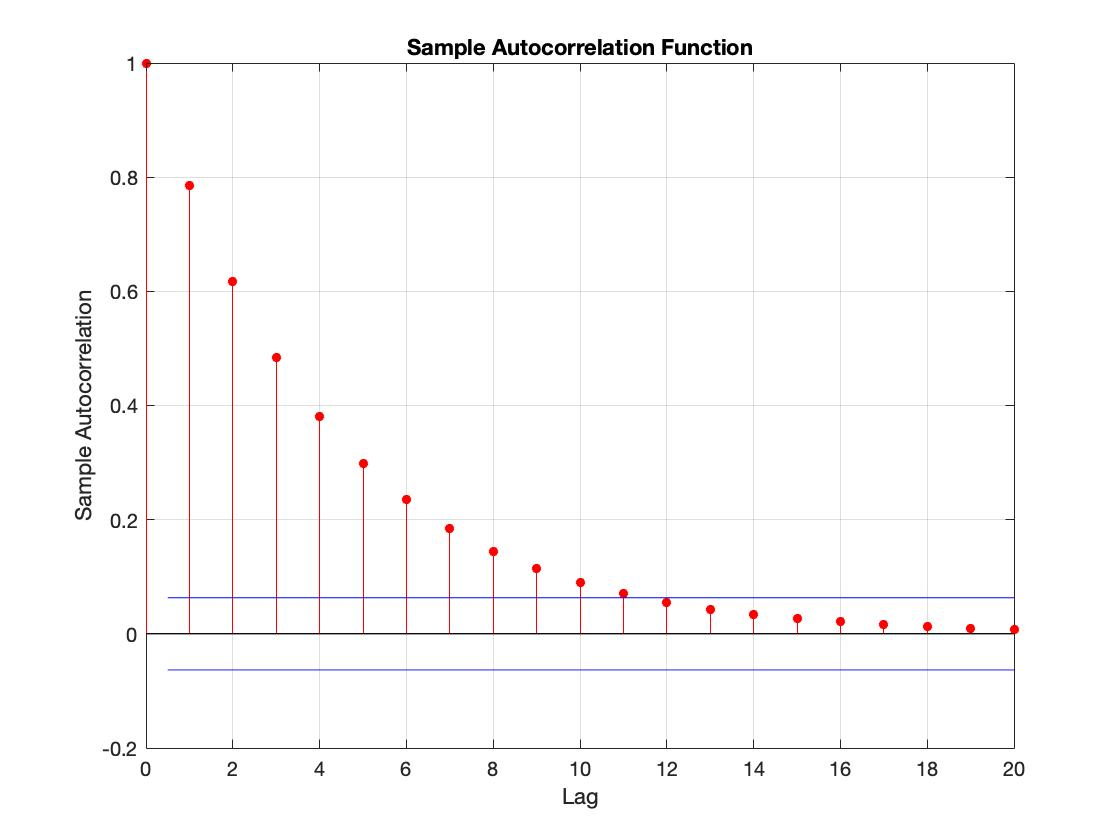
\includegraphics{figures/Fig_331.jpg}
\caption{Autocorrelation Function}
\end{figure}

It looks like after 10 periods the empirical autocorrelation is quite small but still not zero.

\hypertarget{fixed-b-asymptotics}{%
\subsection{Fixed b asymptotics}\label{fixed-b-asymptotics}}

{[}Neave, 1970{]}: ``\emph{When proving results on the asymptotic behavior of estimates of the spectrum of a stationary time series, it is invariably assumed that as the sample size \(n\) tends to infinity, so does the truncation point \(h\), but at a slower rate, so that \(\frac{h}{n}\) tends to zero. This is a convenient assumption mathematically in that, in particular, it ensures consistency of the estimates, but it is unrealistic when such results are used as approximations to the finite case where the value of \(\frac{h}{n}\) cannot be zero.}''"

\textbf{Theorem}:
Under regularity conditions,
\[
    \sqrt{n} \Big( V^{HAC} _ {k,h} \Big)(\hat \beta - \beta_0) \overset{d}{\to} F \\
\]

The asymptotic critical values of the \(F\) statistic depend on the choice of the kernel. In order to do hypothesis testing, Kiefer and Vogelsang(2005) provide critical value functions for the t-statistic for each kernel-confidence level combination using a cubic equation:
\[
    cv(b) = a_0 + a_1 b + a_2 b^2 + a_3 b^3
\]

Example for the Bartlett kernel:

\begin{figure}
\centering
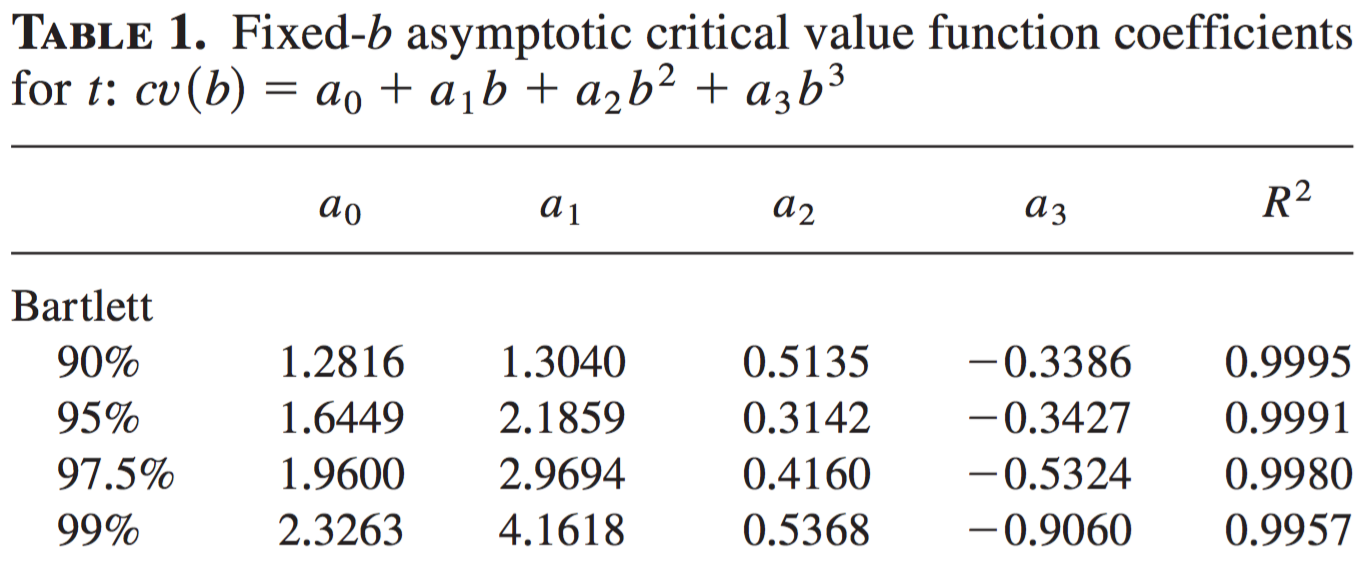
\includegraphics{figures/Fig_332.png}
\caption{Fixed-b}
\end{figure}

\hypertarget{fixed-g-asymptotics}{%
\subsection{Fixed G asymptotics}\label{fixed-g-asymptotics}}

{[}Bester, 2013{]}: ``\emph{Cluster covariance estimators are routinely used with data that has a group structure with independence assumed across groups. Typically, inference is conducted in such settings under the assumption that there are a large number of these independent groups.}''"

``\emph{However, with enough weakly dependent data, we show that groups can be chosen by the researcher so that group-level averages are approximately independent. Intuitively, if groups are large enough and well shaped (e.g.~do not have gaps), the majority of points in a group will be far from other groups, and hence approximately independent of observations from other groups provided the data are weakly dependent. The key prerequisite for our methods is the researcher's ability to construct groups whose averages are approximately independent. As we show later, this often requires that the number of groups be kept relatively small, which is why our main results explicitly consider a fixed (small) number of groups.}''"

\textbf{Assumption}:
Suppose you have data \(D = (y _ {it} , x _ {it}) _ {i=1, t=1}^{N, T}\) where \(y _ {it} = x _ {it}' \beta + \alpha_i + \varepsilon _ {it}\) where \(i\) indexes the observational unit and \(t\) indexes time (could also be space).

Let
\[
\begin{aligned}
  & \tilde{y} _ {it} = y _ {it} - \frac{1}{T} \sum _ {t=1}^T y _ {it} \\
  & \tilde{x} _ {it} = x _ {it} - \frac{1}{T} \sum _ {t=1}^T x _ {it} \\
  & \tilde{\varepsilon} _ {it} = \varepsilon _ {it} - \frac{1}{T} \sum _ {t=1}^T \varepsilon _ {it}
\end{aligned}
\]
Then
\[
\tilde{y} _ {it} = \tilde{x} _ {it}' \beta + \tilde{\varepsilon} _ {it}
\]

The \(\tilde{\varepsilon} _ {it}\) are by construction correlated between each other even if the original \(\varepsilon\) was iid. The \textbf{cluster score variance estimator} is given by:
\[
  \hat{\Omega}^{CL} = \frac{1}{T-1} \sum _ {i=1}^n  \sum _ {t=1}^T  \sum _ {s=1}^T \tilde{x} _ {it} \hat{\tilde{\varepsilon}} _ {it} \tilde{x} _ {is}     \hat{\tilde{\varepsilon}} _ {is}
\]

\begin{quote}
It's very similar too the HAC estimator since we have \emph{dependent cross-products} here as well. However, here we do not consider the \(i \times j\) cross-products. We only have time-dependency (state).
\end{quote}

On \(T\) and \(n\):

\begin{itemize}
\tightlist
\item
  If \(T\) is fixed and \(n \to \infty\), then the number of cross-products considered is much smaller than the total number of cross-products.
\item
  If \(T >> n\) issues arise since the number of cross products considered is close to the total number of cross products. As in HAC estimation, this is a problem because it implies that the algebraic estimate of the cluster score variance gets close to zero because of the orthogonality property of the residuals.
\item
  The panel assumption is that observations across individuals are not correlated.
\end{itemize}

\begin{quote}
Strategy: as in HAC, we want to limit the correlation across clusters (individuals). We hope that observations are \textbf{negligibly dependent} between cluster sufficiently distant from each other.
\end{quote}

Classical cluster robust estimator:
\[
  \hat{\Omega}^{CL} = \frac{1}{n} \sum _ {i=1}^n x_i \varepsilon_i x_j' \varepsilon_j' \mathbb{I}   \\{ i,j \text{ in the same cluster} \\}
\]

\begin{quote}
On clusters:

\begin{itemize}
\tightlist
\item
  If the number of observations near a boundary is small relative to the sample size, ignoring the dependence should not affect inference too adversely.
\item
  The higher the dimension of the data, the easier it is to have observations near boundaries (\emph{curse of dimensionality}).
\item
  We would like to have few clusters in order to make less independence assumptions. However, few clusters means bigger blocks and hence a larger number of cross-products to estimate. If the number of cross-products is too large (relative to the sample size), \(\hat{\Omega}^{CL}\) does not converge
\end{itemize}
\end{quote}

\textbf{Theorem}:
Under regularity conditions:
\[
    \hat{t} \overset{d}{\to} \sqrt{\frac{G}{G-1}} t _ {G-1}
\]

\hypertarget{matlab-4}{%
\subsection{\texorpdfstring{\texttt{Matlab}}{Matlab}}\label{matlab-4}}

\begin{Shaded}
\begin{Highlighting}[]
\CommentTok{% Homoskedastic standard errors}
\NormalTok{std_h = var(e_hat) * inv(X'*X);}

\CommentTok{% HC0 variance and standard errors}
\NormalTok{omega_hc0 = X' * diag(e_hat.^}\FloatTok{2}\NormalTok{) * X;}
\NormalTok{std_hc0 = sqrt(diag(inv(X'*X) * omega_hc0 * inv(X'*X))) }\CommentTok{% = 0.9195, 0.8631}

\CommentTok{% HC1 variance and standard errors}
\NormalTok{omega_hc1 = n/(n-k) * X' *  diag(e_hat.^}\FloatTok{2}\NormalTok{) * X;}
\NormalTok{std_hc1 = sqrt(diag(inv(X'*X) * omega_hc1 * inv(X'*X))) }\CommentTok{% = 0.9289, 0.8719}

\CommentTok{% HC2 variance and standard errors}
\NormalTok{omega_hc2 = X' * diag(e_hat.^}\FloatTok{2}\NormalTok{./(}\FloatTok{1}\NormalTok{-h)) * X;}
\NormalTok{std_hc2 = sqrt(diag(inv(X'*X) * omega_hc2 * inv(X'*X))) }\CommentTok{% = 0.9348, 0.8768}

\CommentTok{% HC3 variance and standard errors}
\NormalTok{omega_hc3 = X' * diag(e_hat.^}\FloatTok{2}\NormalTok{./(}\FloatTok{1}\NormalTok{-h).^}\FloatTok{2}\NormalTok{) * X;}
\NormalTok{std_hc3 = sqrt(diag(inv(X'*X) * omega_hc3 * inv(X'*X))) }\CommentTok{% = 0.9504, 0.8907}

\CommentTok{% Note what happens if you allow for full autocorrelation}
\NormalTok{omega_full = X'*e_hat*e_hat'*X;}
\end{Highlighting}
\end{Shaded}

\hypertarget{inference}{%
\section{Inference}\label{inference}}

In order to do inference on \(\hat \beta\) we need to know its distribution. We have two options: (i) assume gaussian error term (extended GM) or (ii) rely on asymptotic approximations (CLT).

\hypertarget{hypothesis-testing}{%
\subsection{Hypothesis Testing}\label{hypothesis-testing}}

A statistical hypothesis is a subset of a statistical model, \(\mathcal K \subset \mathcal F\). A hypothesis test is a map \(\mathcal D \rightarrow \{ 0,1 \}\), \(D \mapsto T\). If \(\mathcal F\) is the statistical model and \(\mathcal K\) is the statistical hypothesis, we use the notation \(H_0: \Pr \in \mathcal K\).

\begin{quote}
Generally, we are interested in understanding whether it is likely that data \(D\) are drawn from \(\mathcal K\) or not.
\end{quote}

A hypothesis test, \(T\) is our tool for deciding whether the hypothesis is consistent with the data. \(T(D)= 0\) implies fail to reject \(H_0\) and test inconclusive \(T(D)=1\) \(\implies\) reject \(H_0\) and \(D\) is inconsistent with any \(\Pr \in \mathcal K\).

Let \(\mathcal K \subseteq \mathcal F\) be a statistical hypothesis and \(T\) a hypothesis test.

\begin{enumerate}
\def\labelenumi{\arabic{enumi}.}
\tightlist
\item
  Suppose \(\Pr \in \mathcal K\). A Type I error (relative to \(\Pr\)) is an event \(T(D)=1\) under \(\Pr\).\\
\item
  Suppose \(\Pr \in \mathcal K^c\). A Type II error (relative to \(\Pr\)) is an event \(T(D)=0\) under \(\Pr\).
\end{enumerate}

The corresponding probability of a type I error is called \textbf{size}. The corresponding probability of a type II error is called \textbf{power} (against the alternative \(\Pr\)).

In this section, we are interested in testing three hypotheses, under the assumptions of linearity, strict exogeneity, no multicollinearity, normality on the error term. They are:

\begin{enumerate}
\def\labelenumi{\arabic{enumi}.}
\tightlist
\item
  \(H_0: \beta _ {0k} = \bar \beta _ {0k}\) (single coefficient, \(\bar \beta _ {0k} \in \mathbb R\), \(k \leq K\))
\item
  \(a' \beta_0 = c\) (linear combination, \(a \in \mathbb R^K, c \in \mathbb R\))
\item
  \(R \beta_0 = r\) (linear restrictions, \(R \in \mathbb R^{p \times K}\), full rank, \(r \in \mathbb R^p\)) \textbackslash{}
\end{enumerate}

Consider the testing problem
\(H_0: \beta _ {0k} = \bar \beta _ {0k}\) where \(\bar \beta _ {0k}\) is a pre-specified value under the null.
The t-statistic for this problem is defined by
\[
  t_k:= \frac{b_k - \bar \beta _ {0k}}{SE(b_k)}, \ \ SE(b_k):= \sqrt{s^2 [(X'X)^{-1}] _ {kk}}
\]

\textbf{Theorem}: In the testing procedure above, the sampling distribution under the null \(H_0\) is given by
\[
    t_k|X \sim t _ {n-k} \ \ \text{and so} \ \ t_k \sim t _ {n-k} \\
\]

\(t _ {(n-K)}\) denotes the t-distribution with \((n-k)\) degress of freedom. The test can be one sided or two sided. The above sampling distribution can be used to construct a confidence interval.

\textbf{Example}:
We want to asses whether or not the ``true" coefficient \(\beta_0\) equals a specific value \(\hat \beta\). Specifically, we are interested in testing \(H_0\) against \(H_1\), where:

\begin{itemize}
\tightlist
\item
  \emph{Null Hypothesis}: \(H_0: \beta_0 = \hat \beta\)
\item
  \emph{Alternative Hypothesis}: \(H_1: \beta_0 \ne \hat \beta\).
\end{itemize}

Hence, we are interested in a statistic informative about \(H_1\), which is the Wald test statistic
\[
    |T^*| = \bigg| \frac{\hat \beta - \beta_0}{\sigma(\hat \beta)}\bigg|  \sim N(0,1)
\]

However, the true variance \(\sigma^2(\hat \beta )\) is not known and has to be estimated. Therefore we plug in the sample variance \(\hat \sigma^2(\hat \beta) = \frac{n}{n-1} \mathbb E_n[\hat e_i^2]\) and we use
\[
    |T| = \bigg| \frac{\hat \beta - \beta_0}{\hat \sigma (\hat \beta)}\bigg|  \sim t _ {(n-k)}
\]

Hypothesis testing is like proof by contradiction. Imagine the sampling distribution was generated by \(\beta\). If it is highly improbable to observe \(\hat \beta\) given \(\beta_0 = \beta\) then we reject the hypothesis that the sampling distribution was generated by \(\beta\).

Then, given a realized value of the statistic \(|T|\), we take the following decision:

\begin{itemize}
\tightlist
\item
  \emph{Do not reject \(H_0\)}: it is consistent with random variation under true \(H_0\)---i.e., \(|T|\) small as it has an exact student t distribution with \((n-k)\) degree of freedom in the normal regression model.
\item
  \emph{Reject \(H_0\) in favor of \(H_1\)}: \(|T| > c\), with \(c\) being the critical values selected to control for false rejections: \(\Pr(|t _ {n-k}| \geq c) = \alpha\). Moreover, you can also reject \(H_0\) if the p-value \(p\) is such that: \(p < \alpha\).
\end{itemize}

The probability of false rejection is decreasing in \(c\), i.e.~the critical value for a given significant level.
\[
\begin{aligned}
    \Pr (\text{Reject } H_0 | H_0)  & = \Pr (|T|> c | H_0 ) = \\
    & = \Pr (T > c | H_0 ) +     \Pr (T < -c | H_0 ) = \\
    & = 1 - F(c) + F(-c) = 2(1-F(c))
\end{aligned}
\]

\textbf{Example}:
Consider the testing problem \(H_0: a'\beta_0=c\) where \(a\) is a pre-specified linear combination under study. The t-statistic for this problem is defined by:
\[
  t_k:= \frac{a'b - c}{SE(a'b)}, \ \ SE(a'b):= \sqrt{s^2 a'(X'X)^{-1}a}
\]

\textbf{Theorem}:
In the testing procedure above, the sampling distribution under the null \(H_0\) is given by
\[
    t_a|X \sim t _ {n-K} \quad\text{and so} \quad t_a \sim t _ {n-K} 
\]

Like in the previous test, \(t _ {(n-K)}\) denotes the t-distribution with \((n-K)\) degress of freedom. The test can again be one sided or two sided. The above sampling distribution can be used to construct a confidence interval.

\textbf{Example}:
Consider the testing problem
\[
    H_0: R \beta_0 = r
\]
where \(R \in \mathbb R^{p \times k}\) is a presepecified set of linear combinations and \(r \in \mathbb R^p\) is a restriction vector.

The F-statistic for this problem is given by
\[
    F:= \frac{(Rb-r)'[R(X'X)R']^{-1}(Rb-r)/p }{s^2}
\]

\textbf{Theorem}:\\
For the problem, the sampling distribution of the F-statistic under the null \(H_0:\)
\[
    F|X \sim F _ {p,n-K} \ \ \text{and so} \ \ F \sim F _ {p,n-K} \\
\]

The test is intrinsically two-sided. The above sampling distribution can be used to construct a confidence interval.

\textbf{Theorem}:\\
Consider the testing problem \(H_0: R \beta_0 = r\) where \(R \in \mathbb R^{p\times K}\) is a presepecified set of linear combinations and \(r \in \mathbb R^p\) is a restriction vector.

Consider the restricted least squares estimator, denoted \(\hat \beta_R\): \(\hat \beta_R: = \text{arg} \min _ { \beta: R \beta = r } Q( \beta)\). Let \(SSR_U = Q(b), \ \ SSR_R=Q(\hat \beta_R)\). Then the \(F\) statistic is numerically equivalent to the following expression: \(F = \frac{(SSR_R - SSR_U)/p}{SSR_U/(n-K)}\).

\hypertarget{confidence-intervals}{%
\subsection{Confidence Intervals}\label{confidence-intervals}}

A \textbf{confidence interval at \((1-\alpha)\)} is a random set \(C\) such that
\[
     \Pr(\beta_0 \in C) \geq 1- \alpha
\]
i.e.~the probability that \(C\) covers the true value \(\beta\) is fixed at \((1-\alpha)\).

Since \(C\) is not known, it has to be estimated (\(\hat{C}\)). We construct confidence intervals such that:

\begin{itemize}
\tightlist
\item
  they are symmetric around \(\hat \beta\);
\item
  their length is proportional to \(\sigma(\hat \beta) = \sqrt{Var(\hat \beta)}\).
\end{itemize}

A CI is equivalent to the set of parameter values such that the t-statistic is less than \(c\), i.e.,
\[
\hat{C} = \bigg\{ \beta: |T(\beta) | \leq c \bigg\} = \bigg\{ \beta: - c\leq \frac{\beta - \hat \beta}{\sigma(\hat \beta)} \leq c \bigg\}
\]

In practice, to construct a 95\% confidence interval for a single coefficient estimate \(\hat \beta_j\), we use the fact that
\[
    \Pr \left( \frac{| \hat \beta_j - \beta _ {0,j} |}{ \sqrt{\sigma^2 [(X'X)^{-1}] _ {jj} }} > 1.96 \right) = 0.05
\]

\hypertarget{matlab-5}{%
\subsection{\texorpdfstring{\texttt{Matlab}}{Matlab}}\label{matlab-5}}

\begin{Shaded}
\begin{Highlighting}[]
\CommentTok{% t-test for beta=0}
\NormalTok{t = abs(b_hat./(std_hc1));}

\CommentTok{% p-value}
\NormalTok{p_val = }\FloatTok{1}\NormalTok{ - normcdf(t);}

\CommentTok{% F statistic of joint significance}
\NormalTok{SSR_u = e_hat'*e_hat;}
\NormalTok{SSR_r = y'*y;}
\NormalTok{F = (SSR_r - SSR_u)/k / (SSR_u/(n-k));}

\CommentTok{% 95% confidente intervals}
\NormalTok{conf_int = [b_hat - }\FloatTok{1.96}\NormalTok{*std_hc1, b_hat + }\FloatTok{1.96}\NormalTok{*std_hc1];}
\end{Highlighting}
\end{Shaded}

\hypertarget{references-5}{%
\section{References}\label{references-5}}

\begin{itemize}
\tightlist
\item
  Kozbur (2019). PhD Econometrics - Lecture Notes.
\item
  Hansen (2019). ``\emph{Econometrics}''.
\item
  Kiefer and Vogelsang (2005). ``\emph{A new asymptotic theory for heteroskedasticity-autocorrelation robust tests}''.
\item
  Wooldridge (2010). ``\emph{Econometric Analysis of Cross Section and Panel Data}''.
\item
  Greene (2006). ``\emph{Econometric Analysis}''.
\item
  Hayiashi (2000). ``\emph{Econometrics}''.
\end{itemize}

\hypertarget{lecture3}{%
\chapter{Endogeneity}\label{lecture3}}

\hypertarget{instrumental-variables}{%
\section{Instrumental Variables}\label{instrumental-variables}}

We say that there is \textbf{endogeneity} in the linear regression model if \(\mathbb E[x_i \varepsilon_i] \neq 0\).

The random vector \(z_i\) is an \textbf{instrumental variable} in the linear regression model if the following conditions are met.

\begin{itemize}
\tightlist
\item
  \textbf{Exclusion restriction}: the instruments are uncorrelated with the regression error
  \[
    \mathbb E_n[z_i \varepsilon_i] = 0 
  \]
  almost surely, i.e.~with probability \(p \to 1\).
\item
  \textbf{Rank condition}: no linearly redundant instruments
  \[ 
    \mathbb E_n[z_i z_i'] \neq 0 
  \]
  almost surely, i.e.~with probability \(p \to 1\).
\item
  \textbf{Relevance condition} (need \(L > K\)):
  \[
    rank \ (\mathbb E_n[z_i x_i']) = K
  \]
  almost surely, i.e.~with probability \(p \to 1\).
\end{itemize}

Let \(K = dim(x_i)\) and \(L = dim(z_i)\). We say that the model is \textbf{just-identified} if \(L = K\) (method: IV) and \textbf{over-identified} if \(L > K\) (method: 2SLS).

Assume \(z_i\) satisfies the instrumental variable assumptions above and \(dim(z_i) = dim(x_i)\), then the \textbf{instrumental variables (IV)} estimator \(\hat{\beta} _ {IV}\) is given by
\[
\begin{aligned}
    \hat{\beta} _ {IV} &= \mathbb E_n[z_i x_i']^{-1} \mathbb E_n[z_i y_i] = \\
    &= \left( \frac{1}{n} \sum _ {i=1}^n z_i x_i\right)^{-1} \left( \frac{1}{n} \sum _ {i=1}^n z_i y_i\right) = \\
    &= (Z'X)^{-1} (Z'y) 
\end{aligned}
\]

Assume \(z_i\) satisfies the instrumental variable assumptions above and \(dim(z_i) > dim(x_i)\), then the \textbf{two-stage-least squares (2SLS)} estimator \(\hat{\beta} _ {2SLS}\) is given by
\[
    \hat{\beta} _ {2SLS} =  \Big( X'Z (Z'Z)^{-1} Z'X \Big)^{-1} \Big( X'Z (Z'Z)^{-1} Z'y \Big)
\]
Where \(\hat{x}_i\) is the predicted \(x_i\) from the \textbf{first stage} regression of \(x_i\) on \(z_i\). This is equivalent of the IV estimator using \(\hat{x}_i\) as an instrument for \(x_i\).

\begin{quote}
On the algebra of 2SLS:

\begin{itemize}
\tightlist
\item
  The estimator is called \textit{two-stage-least squares} since it can be rewritten as an IV estimator that uses \(\hat{X}\) as instrument:
  \[
  \begin{aligned}
  \hat{\beta} _ {\text{2SLS}} &= \Big( X'Z (Z'Z)^{-1} Z'X \Big)^{-1} \Big( X'Z (Z'Z)^{-1} Z'y \Big) = \\
  &= (\hat{X}' X)^{-1} \hat{X}' y = \\
  &= \mathbb E_n[\hat{x}_i x_i']^{-1} \mathbb E_n[\hat{x}_i y_i] 
  \end{aligned}
  \]
\item
  Moreover it can be rewritten as
  \[
  \begin{aligned}
  \hat{\beta} _ {\text{2SLS}} &= (\hat{X}' X)^{-1} \hat{X}' y = \\
  &= (X' P_Z X)^{-1} X' P_Z y = \\
  &= (X' P_Z P_Z X)^{-1} X' P_Z y = \\
  &= (\hat{X}' \hat{X})^{-1} \hat{X}' y = \\
  &= \mathbb E_n [\hat{x}_i \hat{x}_i]^{-1} \mathbb E_n[\hat{x}_i y_i] 
  \end{aligned}
  \]
\item
  How to the test the relevance condition? Rule of thumb: \(F\)-test in the first stage \(>10\) (joint test on \(z_i\)).
  \textbf{Problem}: as \(n \to \infty\), with finite \(L\), \(F \to \infty\) (bad rule of thumb).
\end{itemize}
\end{quote}

\textbf{Theorem}:
If \(K=L\), \(\hat{\beta} _ {\text{2SLS}} = \hat{\beta} _ {\text{IV}}\).

\textbf{Proof}:
If \(K=L\), \(X'Z\) and \(Z'X\) are squared matrices and, by the relevance condition, non-singular (invertible).
\[
\begin{aligned}
    \hat{\beta} _ {\text{2SLS}} &= \Big( X'Z (Z'Z)^{-1} Z'X \Big)^{-1} \Big( X'Z (Z'Z)^{-1} Z'y \Big) = \\
    &= (Z'X)^{-1} (Z'Z) (X'Z)^{-1} X'Z (Z'Z)^{-1} Z'y = \\
    &= (Z'X)^{-1} (Z'Z) (Z'Z)^{-1} Z'y = \\
    &= (Z'X)^{-1} (Z'y) = \\
    &= \hat{\beta} _ {\text{IV}}
\end{aligned}
\]
\[\tag*{$\blacksquare$}\]

\begin{quote}
\textbf{Example} from Hayiashi (2000) page 187: demand and supply simultaneous equations.
\[
\begin{aligned}
& q_i^D(p_i) = \alpha_0 + \alpha_1 p_i + u_i \\
& q_i^S(p_i) = \beta_0 + \beta_1 p_i + v_i 
\end{aligned}
\]

We have an endogeneity problem. To see why, we solve the system of equations for \((p_i, q_i)\):
\[
\begin{aligned}
& p_i = \frac{\beta_0 - \alpha_0}{\alpha_1 - \beta_1} + \frac{v_i - u_i}{\alpha_1 - \beta_1 } \\
& q_i = \frac{\alpha_1\beta_0 - \alpha_0 \beta_1}{\alpha_1 - \beta_1} + \frac{\alpha_1 v_i - \beta_1 u_i}{\alpha_1 - \beta_1 } 
\end{aligned}
\]

Then the price variable is not independent from the error term in neither equation:
\[
\begin{aligned}
& Cov(p_i, u_i) = - \frac{Var(u_i)}{\alpha_1 - \beta_1 } \\
& Cov(p_i, v_i) = \frac{Var(v_i)}{\alpha_1 - \beta_1 } 
\end{aligned}
\]

As a consequence, the two coefficient estimates are not consistent:
\[
\begin{aligned}
& \hat{\alpha} _ {1, OLS} \overset{p}{\to} \alpha_1 + \frac{Cov(p_i, u_i)}{Var(p_i)} \\
& \hat{\beta} _ {1, OLS} \overset{p}{\to} \beta_1 + \frac{Cov(p_i, v_i)}{Var(p_i)} 
\end{aligned}
\]

In general, running OLS on \(q_i = \gamma p_i + \varepsilon_i\) you estimate
\[
\begin{aligned}
\hat{\gamma} _ {OLS} &\overset{p}{\to} \frac{Cov(p_i, q_i)}{Var(p_i)} = \\
&= \frac{\alpha_1 Var(v_i) + \beta_1 Var(u_i)}{(\alpha_1 - \beta_1)^2} \left( \frac{Var(v_i) + Var(u_i)}{(\alpha_1 - \beta_1)^2} \right)^{-1} = \\
&= \frac{\alpha_1 Var(v_i) + \beta_1 Var(u_i)}{Var(v_i) + Var(u_i)} 
\end{aligned}
\]

Which is neither \(\alpha_1\) nor \(\beta_1\) but a variance weighted average of the two.

Suppose we have a supply shifter \(z_i\) such that \(\mathbb E[z_i v_i] \neq 0\) and \(\mathbb E[z_i u_i] = 0\). We combine the second condition and \(\mathbb E[u_i] = 0\) to get a system of 2 equations in 2 unknowns: \(\alpha_0\) and \(\alpha_1\).
\[
\begin{aligned}
& \mathbb E[z_i u_i] = \mathbb E[ z_i (q_i^D(p_i) - \alpha_0 - \alpha_1 p_i) ] = 0 \\
& \mathbb E[u_i] = \mathbb E[q_i^D(p_i) - \alpha_0 - \alpha_1 p_i] = 0  
\end{aligned}
\]

We could try to solve for the vector \(\alpha\) that solves
\[
\begin{aligned}
& \mathbb E_n[z_i (q_i^D - x_i\alpha)] = 0 \\
& \mathbb E_n[z_i q_i^D] -  \mathbb E_n[z_ix_i\alpha] = 0 
\end{aligned}
\]

If \(\mathbb E_n[z_ix_i]\) is invertible, we get \(\hat{\alpha} = \mathbb E_n[z_ix_i]^{-1} \mathbb E_n[z_i q^D_i]\) which is indeed the IV estimator of \(\alpha\) using \(z_i\) as an instrument for the endogenous variable \(p_i\).
\end{quote}

\hypertarget{matlab-6}{%
\subsection{\texorpdfstring{\texttt{Matlab}}{Matlab}}\label{matlab-6}}

\begin{Shaded}
\begin{Highlighting}[]
\CommentTok{% Set the dimension of Z}
\NormalTok{l = }\FloatTok{3}\NormalTok{;}

\CommentTok{% Draw instruments}
\NormalTok{Z = randn(n,l);}

\CommentTok{% Correlation matrix for error terms}
\NormalTok{S = eye(}\FloatTok{2}\NormalTok{,}\FloatTok{2}\NormalTok{); S(}\FloatTok{1}\NormalTok{,}\FloatTok{2}\NormalTok{)=}\FloatTok{.8}\NormalTok{; S(}\FloatTok{2}\NormalTok{,}\FloatTok{1}\NormalTok{)=}\FloatTok{.8}\NormalTok{; }

\CommentTok{% Endogenous X}
\NormalTok{gamma = [}\FloatTok{2}\NormalTok{, }\FloatTok{0}\NormalTok{; }\FloatTok{0}\NormalTok{, -}\FloatTok{1}\NormalTok{; -}\FloatTok{1}\NormalTok{, }\FloatTok{3}\NormalTok{];}
\NormalTok{e = randn(n,}\FloatTok{2}\NormalTok{)*chol(S);}
\NormalTok{X = Z*gamma + e(:,}\FloatTok{1}\NormalTok{);}

\CommentTok{% Calculate Y}
\NormalTok{Y = X*b + e(:,}\FloatTok{2}\NormalTok{);}

\CommentTok{% Estimate beta OLS}
\NormalTok{beta_OLS = (X'*X)\textbackslash{}(X'*Y) }\CommentTok{% = 2.1957, -0.9022}

\CommentTok{% IV: l=k=2 instruments}
\NormalTok{Z_IV = Z(:,}\FloatTok{1}\NormalTok{:k);}
\NormalTok{beta_IV = (Z_IV'*X)\textbackslash{}(Z_IV'*Y) }\CommentTok{% = 2.1207, -1.3617}

\CommentTok{% Calculate standard errors}
\NormalTok{ehat = Y - X*beta_IV;}
\NormalTok{V_NHC_IV = var(ehat) * inv(Z_IV'*X)*Z_IV'*Z_IV*inv(Z_IV'*X);}
\NormalTok{V_HC0_IV = inv(Z_IV'*X)*Z_IV' * diag(ehat.^}\FloatTok{2}\NormalTok{) * Z_IV*inv(Z_IV'*X);}

\CommentTok{% 2SLS: l=3 instruments}
\NormalTok{Pz = Z*inv(Z'*Z)*Z';}
\NormalTok{beta_2SLS = (X'*Pz*X)\textbackslash{}(X'*Pz*Y) }\CommentTok{% = 2.0723, -0.9628}

\CommentTok{% Calculate standard errors}
\NormalTok{ehat = Y - X*beta_2SLS;}
\NormalTok{V_NCH_2SLS = var(ehat) * inv(X'*Pz*X);}
\NormalTok{V_HC0_2SLS = inv(X'*Pz*X)*X'*Pz * diag(ehat.^}\FloatTok{2}\NormalTok{) *Pz*X*inv(X'*Pz*X);}
\end{Highlighting}
\end{Shaded}

\hypertarget{gmm}{%
\section{GMM}\label{gmm}}

Setting: we have a system of \(L\) moment conditions
\[
\begin{aligned}
    & \mathbb E[g_1(\omega_i, \delta_0)] = 0 \\
    & \vdots \\
    & \mathbb E[g_L(\omega_i, \delta_0)] = 0
\end{aligned}
\]

If \(L = \dim (\delta_0)\), no problem. If \(L > \dim (\delta_0)\), there may be no solution to the system of equations. There are two possibilities.

\begin{enumerate}
\def\labelenumi{\arabic{enumi}.}
\tightlist
\item
  \textbf{First Solution}: add moment conditions until the system is identified
  \[
     \mathbb E[ a' g(\omega_i, \delta_0)] = 0
   \]
  Solve \(\mathbb E[Ag(\omega_i, \delta)] = 0\) for \(\hat{\delta}\). How to choose \(A\)? Such that it minimizes \(Var(\hat{\delta})\).\\
\item
  \textbf{Second Solution}: generalized method of moments (GMM)
  \[
   \begin{aligned}
     \hat{\delta} _ {GMM} &= \arg \min _ \delta \quad  \Big| \Big| \mathbb E_n [ g(\omega_i, \delta) ] \Big| \Big| = \\
     &= \arg \min _ \delta \quad n \mathbb E_n[g(\omega_i, \delta)]' W \mathbb E_n [g(\omega_i, \delta)]
   \end{aligned}
   \]
\end{enumerate}

\begin{quote}
The choice of \(A\) and \(W\) are closely related to each other.
\end{quote}

\hypertarget{step-gmm}{%
\subsection{1-step GMM}\label{step-gmm}}

Since \(J(\delta,W)\) is a quadratic form, a closed form solution exists:
\[
    \hat{\delta}(W) = \Big(\mathbb E_n[z_i x_i'] W \mathbb E_n[z_i x_i'] \Big)^{-1}\mathbb E_n[z_i x_i'] W \mathbb E_n[z_i y_i]
\]

\textbf{Assumptions} for consistency of the GMM estimator given data \(\mathcal D = \{y_i, x_i, z_i \} _ {i=1}^n\):

\begin{itemize}
\tightlist
\item
  \textbf{Linearity}: \(y_i = x_i\gamma_0 + \varepsilon_i\)
\item
  \textbf{IID}: \((y_i, x_i, z_i)\) iid
\item
  \textbf{Orthogonality}: \(\mathbb E [z_i(y_i - x_i\gamma_0)] = \mathbb E[z_i \varepsilon_i] = 0\)
\item
  \textbf{Rank identification}: \(\Sigma_{xz} = \mathbb E[z_i x_i']\) has full rank
\end{itemize}

\textbf{Theorem}:
Under linearity, independence, orthogonality and rank conditions, if \(\hat{W} \overset{p}{\to} W\) positive definite, then
\[
    \hat{\delta}(\hat{W}) \to \delta(W)
\]
If in addition to the above assumption, \(\sqrt{n} \mathbb E_n [g(\omega_i, \delta_0)] \overset{d}{\to} N(0,S)\) for a fixed positive definite \(S\), then
\[
    \sqrt{n} (\hat{\delta} (\hat{W}) - \delta(W)) \overset{d}{\to} N(0,V)
\]
where \(V = (\Sigma' _ {xz} W \Sigma _ {xz})^{-1} \Sigma _ {xz} W S W \Sigma _ {xz}(\Sigma' _ {xz} W \Sigma _ {xz})^{-1}\).

Finally, if a consistent estimator \(\hat{S}\) of \(S\) is available, then using sample analogues \(\hat{\Sigma}_{xz}\) it follows that
\[
    \hat{V} \overset{p}{\to} V
\]

\begin{quote}
If \(W = S^{-1}\) then \(V\) reduces to \(V = (\Sigma' _ {xz} W \Sigma _ {xz})^{-1}\). Moreover, \((\Sigma' _ {xz} W \Sigma _ {xz})^{-1}\) is the smallest possible form of \(V\), in a positive definite sense.
\end{quote}

Therefore, to have an efficient estimator, you want to construct \(\hat{W}\) such that \(\hat{W} \overset{p}{\to} S^{-1}\).

\hypertarget{step-gmm-1}{%
\subsection{2-step GMM}\label{step-gmm-1}}

Estimation steps:

\begin{itemize}
\tightlist
\item
  Choose an arbitrary weighting matrix \(\hat{W}_{init}\) (usually the identity matrix \(I_K\))
\item
  Estimate \(\hat{\delta} _ {init}(\hat{W} _ {init})\)
\item
  Estimate \(\hat{S}\) (asymptotic variance of the moment condition)
\item
  Estimate \(\hat{\delta}(\hat{S}^{-1})\)
\end{itemize}

\begin{quote}
On the procedure:

\begin{itemize}
\tightlist
\item
  This estimator achieves the semiparametric efficiency bound.
\item
  This strategy works only if \(\hat{S} \overset{p}{\to} S\) exists.
\item
  For iid cases: we can use \(\hat{\delta} = \mathbb E_n[(\hat{\varepsilon}_i z_i)(\hat{\varepsilon}_i z_i) ' ]\) where \(\hat{\varepsilon}_i = y_i - x_i \hat{\delta}(\hat{W} _ {init})\).
\end{itemize}
\end{quote}

\hypertarget{matlab-7}{%
\subsection{\texorpdfstring{\texttt{Matlab}}{Matlab}}\label{matlab-7}}

\begin{Shaded}
\begin{Highlighting}[]
\CommentTok{% GMM 1-step: inefficient weighting matrix}
\NormalTok{W_1 = eye(l);}

\CommentTok{% Objective function}
\NormalTok{gmm_1 = @(b) ( Y - X*b )' * Z * W_1 *  Z' * ( Y - X*b );}

\CommentTok{% Estimate GMM}
\NormalTok{beta_gmm_1 = fminsearch(gmm_1, beta_OLS) }\CommentTok{% = 2.0763, -0.9548}
\NormalTok{ehat = Y - X*beta_gmm_1;}

\CommentTok{% Standard errors GMM}
\NormalTok{S_hat = Z'*diag(ehat.^}\FloatTok{2}\NormalTok{)*Z;}
\NormalTok{d_hat = -X'*Z;}
\NormalTok{V_gmm_1 = inv(d_hat * inv(S_hat) * d_hat');}

\CommentTok{% GMM 2-step: efficient weighting matrix}
\NormalTok{W_2 = inv(S_hat);}
\NormalTok{gmm_2 = @(b) ( Y - X*b )' * Z * W_2 *  Z' * ( Y - X*b );}
\NormalTok{beta_gmm_2 = fminsearch(gmm_2, beta_OLS) }\CommentTok{% = 2.0595, -0.9666}

\CommentTok{% Standard errors GMM}
\NormalTok{ehat = Y - X*beta_gmm_2;}
\NormalTok{S_hat = Z'*diag(ehat.^}\FloatTok{2}\NormalTok{)*Z;}
\NormalTok{d_hat = -X'*Z;}
\NormalTok{V_gmm_2 = inv(d_hat * inv(S_hat) * d_hat');}
\end{Highlighting}
\end{Shaded}

\hypertarget{testing-overidentifying-restrictions}{%
\section{Testing Overidentifying Restrictions}\label{testing-overidentifying-restrictions}}

If the equations are \textbf{exactly identified}, then it is possible to choose \(\delta\) so that all the elements of the sample moments \(\mathbb E_n[g(\omega_i; \delta)]\) are zero and thus that the distance
\[
J(\delta, \hat{W}) = n \mathbb E_n[g(\omega_i, \delta)]' \hat{W} \mathbb E_n[g(\omega_i, \delta)]
\]
is zero. (The \(\delta\) that does it is the IV estimator.)

If the equations are \textbf{overidentified}, i.e.~\(L\) (number of instruments) \(> K\) (number of equations), then the distance cannot be zero exactly in general, but we would expect the minimized distance to be \emph{close} to zero.

\hypertarget{naive-test}{%
\subsection{Naive Test}\label{naive-test}}

Suppose your model is overidentified (\(L > K\)) and you use the following naive testing procedure:

\begin{enumerate}
\def\labelenumi{\arabic{enumi}.}
\tightlist
\item
  Estimate \(\hat{\delta}\) using a subset of dimension \(K\) of instruments \(\{z_1 , .. , z_K\}\) for \(\{x_1 , ... , x_K\}\)
\item
  Set \(\hat{\varepsilon}_i = y_i - x_i \hat{\delta} _ {\text{GMM}}\)
\item
  Infer the size of the remaining \(L-K\) moment conditions \(\mathbb E[z _{i, K+1} \varepsilon_i], ..., \mathbb E[z _{i, L} \varepsilon_i]\) looking at their empirical counterparts \(\mathbb E_n[z _{i, K+1} \hat{\varepsilon}_i], ..., \mathbb E_n[z _{i, L} \hat{\varepsilon}_i]\)
\item
  Reject exogeneity if the empirical expectations are high. How high? Calculate p-values.
\end{enumerate}

\begin{quote}
\textbf{Example}
If you have two invalid instruments and you use one to test the validity of the other, it might happen by chance that you don't reject it.

\begin{itemize}
\tightlist
\item
  Model: \(y_i = x_i + \varepsilon_i\) and \(x_i = \frac{1}{2} z _{i1} - \frac{1}{2} z _{i2} + u_i\)
\item
  Have \[
  Cov (z _{i1}, z _{i2}, \varepsilon_i, u_i) = 
  \begin{bmatrix}
  1 & 0 & 0 & 0 \\ 0 & 1 & 0 & 0 \\ 0 & 0 & 1 & 0.5 \\ 0 & 0 & 0.5 & 1 
  \end{bmatrix}
  \]
\item
  You want to test whether the second instrument is valid (is not since \(\mathbb E[z_2 \varepsilon] \neq 0\)).
  You use \(z_1\) and estimate \(\hat{\beta} \to\) the estimator is consistent.
\item
  You obtain \(\mathbb E_n[z _{i2} \hat{\varepsilon}_i] \simeq 0\) even if \(z_2\) is invalid
\item
  Problem: you are using an invalid instrument in the first place.
\end{itemize}
\end{quote}

\hypertarget{hansens-test}{%
\subsection{Hansen's Test}\label{hansens-test}}

\textbf{Theorem}:
We are interested in testing \(H_0: \mathbb E[z_i \varepsilon_i] = 0\) against \(H_1: \mathbb E[z_i \varepsilon_i] \neq 0\). Suppose \(\hat{S} \overset{p}{\to} S\). Then
\[
    J(\hat{\delta}(\hat{S}^{-1}) , \hat{S}^{-1}) \overset{d}{\to} \chi^2 _ {L-K}
\]
For \(c\) satisfying \(\alpha = 1- G_{L - K} ( c )\), \(\Pr(J>c | H_0) \to \alpha\) so the test \emph{reject \(H_0\) if \(J > c\)} has asymptotic size \(\alpha\).

\begin{quote}
On Hansen's test:

\begin{itemize}
\tightlist
\item
  The degrees of freedom of the asymptotic distribution are the number of overidentifying restrictions.
\item
  This is a specification test, testing whether all model assumptions are true jointly. Only when we are confident that about the other assumptions, can we interpret a large \(J\) statistic as evidence for the endogeneity of some of the \(L\) instruments included in \(x\).
\item
  Unlike the tests we have encountered so far, the test is not consistent against some failures of the orthogonality conditions (that is, it is not consistent against some fixed elements of the alternative).
\item
  Several papers in the July 1996 issue of JBES report that the finite-sample null rejection probability of the test can far exceed the nominal significance level \(\alpha\).
\end{itemize}
\end{quote}

\hypertarget{special-case-conditional-homoskedasticity}{%
\subsection{Special Case: Conditional Homoskedasticity}\label{special-case-conditional-homoskedasticity}}

The main implication of conditional homoskedasticity is that efficient GMM becomes 2SLS. With efficient GMM estimation, the weighting matrix is \(\hat{S}^{-1} = \mathbb En [z_i z_i' \varepsilon_i^2]^{-1}\). With conditional homoskedasticity, the efficient weighting matrix is \(\mathbb E_n[z_iz_i']^{-1} \sigma^{-2}\), or equivalently \(\mathbb E_n[z_iz_i']^{-1}\). Then, the GMM estimator becomes
\[
    \hat{\delta}(\hat{S}^{-1}) = \Big(\mathbb E_n[z_i x_i']' \underbrace{\mathbb E_n[z_iz_i']^{-1} \mathbb E[z_i x_i']} _ {\text{ols of } x_i \text{ on }z_i} \Big)^{-1}\mathbb E_n[z_i x_i']' \underbrace{\mathbb E_n[z_iz_i']^{-1} \mathbb E[z_i y_i']} _ {\text{ols of } y_i \text{ on }z_i}= \hat{\delta} _ {2SLS}
\]

\textbf{Proof}:
Consider the matrix notation.
\[
\begin{aligned}
    \hat{\delta} \left( \frac{Z'Z}{n}\right) &= \left( \frac{X'Z}{n} \left( \frac{Z'Z}{n}\right)^{-1} \frac{Z'X}{n} \right)^{-1} \frac{X'Z}{n} \left( \frac{Z'Z}{n}\right)^{-1} \frac{Z'Y}{n} = \\
    &= \left( X'Z(Z'Z)^{-1} Z'X \right)^{-1} X'Z(Z'Z)^{-1} Z'Y = \\
    &= \left(X'P_ZX\right)^{-1} X'P_ZY = \\
    &= \left(X'P_ZP_ZX\right)^{-1} X'P_ZY = \\
    &= \left(\hat{X}'_Z \hat{X}_Z\right)^{-1} \hat{X}'_ZY = \\
    &= \hat{\delta} _ {2SLS}
\end{aligned}
\]
\[\tag*{$\blacksquare$}\]

\hypertarget{small-sample-properties-of-2sls}{%
\section{Small-Sample Properties of 2SLS}\label{small-sample-properties-of-2sls}}

\textbf{Theorem}:
When the number of instruments is equal to the sample size (\(L = n\)), then \(\hat{\delta} _ {2SLS} = \hat{\delta} _ {OLS}\)

\textbf{Proof}:
We have a perfect prediction problem. The first stage estimated coefficient \(\hat{\gamma}\) is such that it solves the normal equations: \(\hat{\gamma} = z_i^{-1} x_i\). Then
\[
\begin{aligned}
    \hat{\delta} _ {2SLS} &= \mathbb E_n[\hat{x}_i x'_i]^{-1} \mathbb E_n[\hat{x}_i y_i] = \\
    &= \mathbb E_n[z_i z_i^{-1} x_i x'_i]^{-1} \mathbb E_n[z_i z_i^{-1} x_i y_i] = \\
    &= \mathbb E_n[x_i x'_i]^{-1} \mathbb E_n[x_i y_i] = \\
    &= \hat{\delta} _ {OLS}
\end{aligned}
\]
\[\tag*{$\blacksquare$}\]

\begin{quote}
You have this overfitting problem in general when the number of instruments is large relative to the sample size. This problem arises even if the instruments are valid.
\end{quote}

\begin{quote}
\textbf{Example} from Angrist (1992)

\begin{itemize}
\tightlist
\item
  They regress wages on years of schooling.
\item
  Problem: endogeneity: both variables are correlated with skills which are unobserved.
\item
  Solution: instrument years of schooling with the quarter of birth. Idea: if born in the first three quarters, can attend school from the year of your sixth birthday. Otherwise, you have to wait one more year.
\item
  Problem: quarters of birth are three dummies. In order to ``improve the first stage fit" they interact them with year of birth (180 effective instruments) and also with the state (1527 effective instruments). This mechanically increases the \(R^2\) but also increases the bias of the 2SLS estimator.
\item
  Solutions: LIML, JIVE, RJIVE (Hansen et al., 2014), Post-Lasso (Belloni et al., 2012).
\end{itemize}
\end{quote}

\begin{figure}
\centering
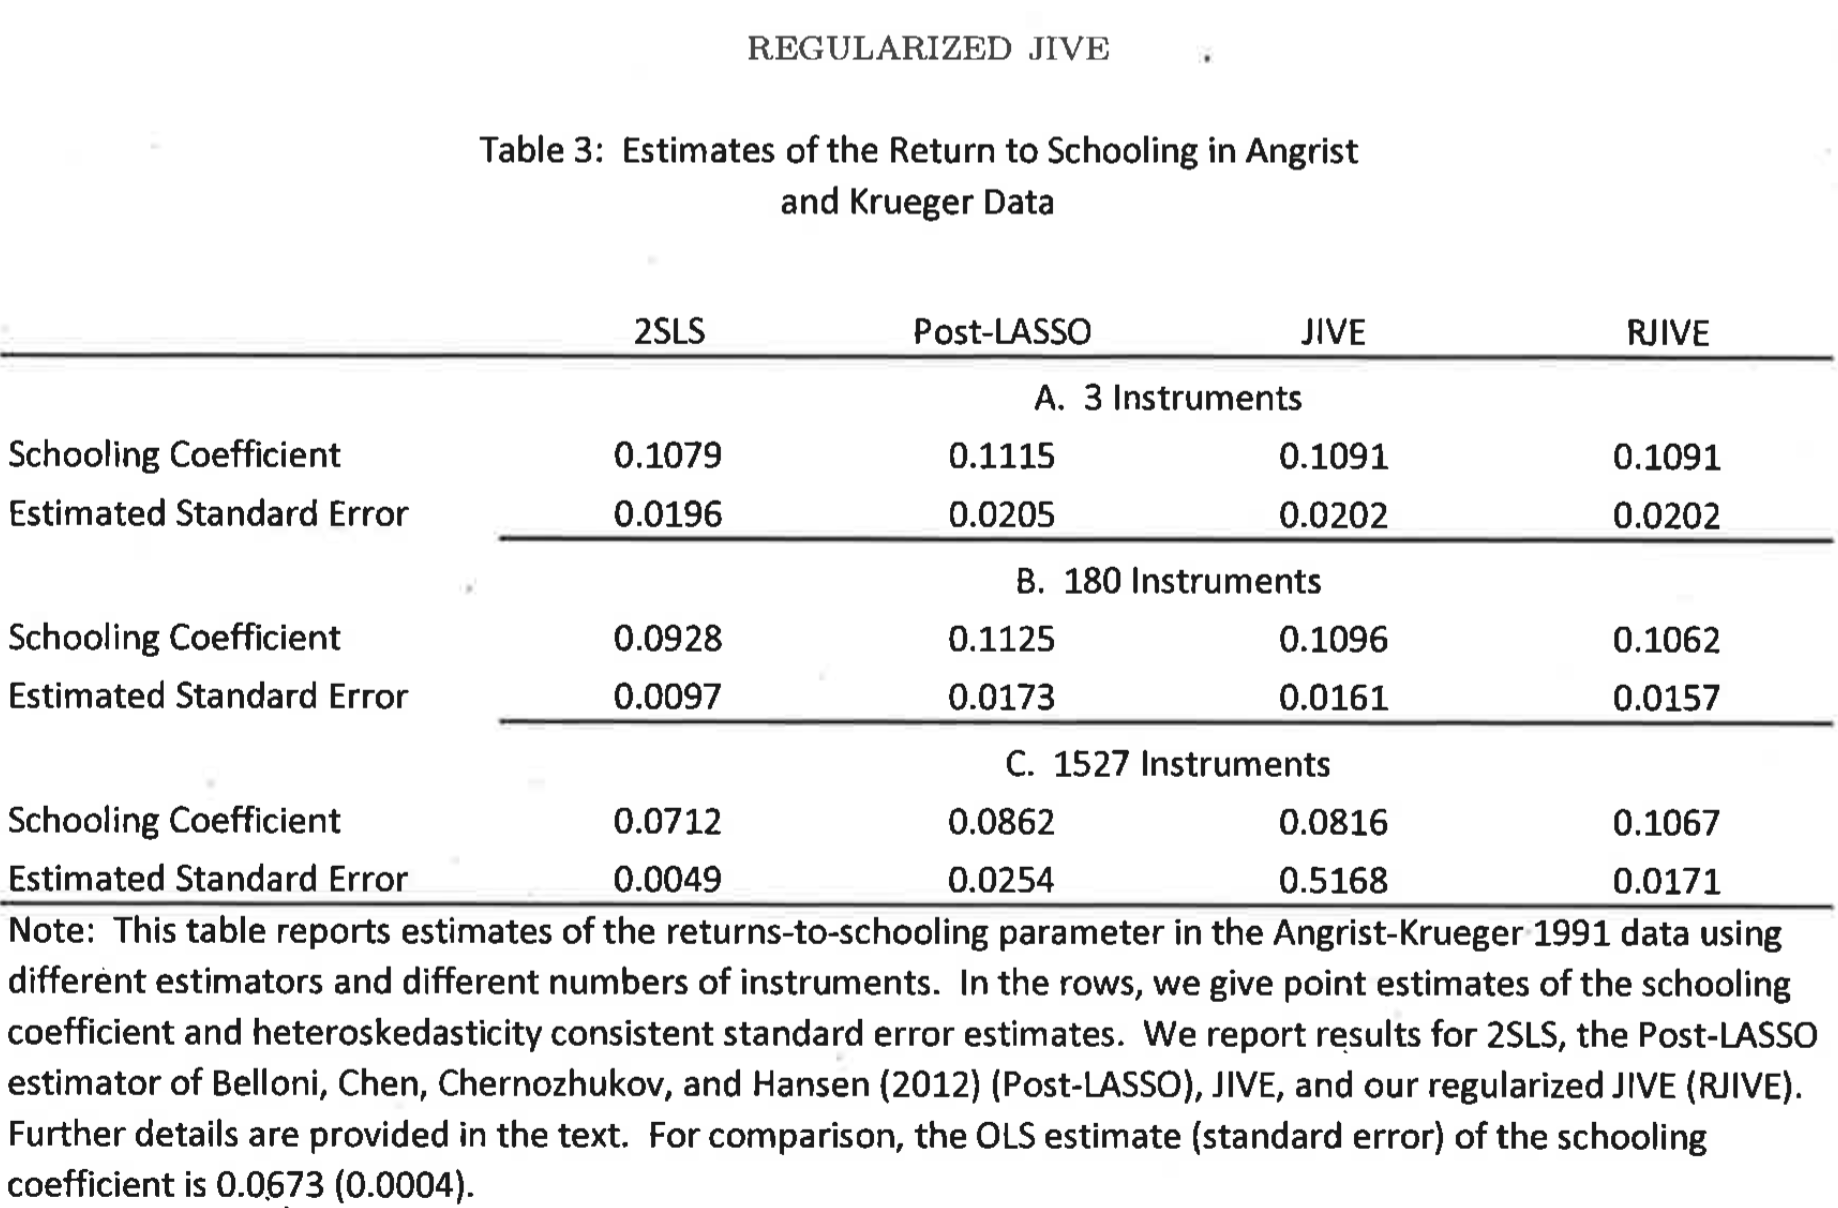
\includegraphics{figures/Fig_441.png}
\caption{RJIVE}
\end{figure}

\hypertarget{many-instrument-robust-estimation}{%
\section{Many Instrument Robust Estimation}\label{many-instrument-robust-estimation}}

Why having too many instruments is problematic? As the number of instruments increases, the estimated coefficient gets closer to OLS which is biased. As seen in the theorem above, for \(L=n\), the two estimators coincide.

\begin{figure}
\centering
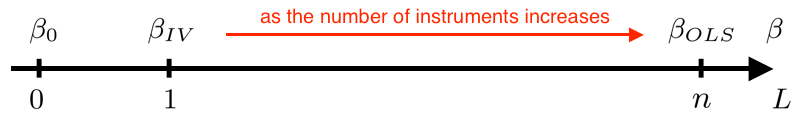
\includegraphics{figures/Fig_451.png}
\caption{IV to OLS}
\end{figure}

\hypertarget{liml}{%
\subsection{LIML}\label{liml}}

An alternative method to estimate the parameters of the structural equation is by maximum likelihood. Anderson and Rubin (1949) derived the maximum likelihood estimator for the joint distribution of \((y_i, x_i)\). The estimator is known as \textbf{limited information maximum likelihood}, or \textbf{LIML}.
This estimator is called ``limited information" because it is based on the structural equation for \((y_i, x_i)\) combined with the reduced form equation for \(x_i\). If maximum likelihood is derived based on a structural equation for \(x_i\) as well, then this leads to what is known as \textbf{full information maximum likelihood (FIML)}. The advantage of the LIML approach relative to FIML is that the former does not require a structural model for \(x_i\), and thus allows the researcher to focus on the structural equation of interest - that for \(y_i\).

The \textbf{k-class} estimators have the form
\[
    \hat{\delta}(\alpha) = (X' P_Z X - \alpha X' X)^{-1} (X' P_Z Y - \alpha X' Y) 
\]

The limited information maximum likelihood estimator \textbf{LIML} is the k-class estimator \(\hat{\delta}(\alpha)\) where
\[
    \alpha = \lambda_{min} \Big( ([X' , Y]^{-1} [X' , Y])^{-1} [X' , Y]^{-1} P_Z [X' , Y] \Big) 
\]

If \(\alpha = 0\) then \(\hat{\delta} _ {\text{LIML}} = \hat{\delta} _ {\text{2SLS}}\) while for \(\alpha \to \infty\), \(\hat{\delta} _ {\text{LIML}} \to \hat{\delta} _ {\text{OLS}}\).

\begin{quote}
Comments on LIML:

\begin{itemize}
\tightlist
\item
  The particular choice of \(\alpha\) gives a many instruments robust estimate
\item
  The LIML estimator has no finite sample moments. \(\mathbb E[\delta(\alpha_{LIML})]\) does not exist in general
\item
  In simulation studies performs well
\item
  Has good asymptotic properties
\end{itemize}
\end{quote}

Asymptotically the LIML estimator has the same distribution as 2SLS. However, they can have quite different behaviors in finite samples. There is considerable evidence that the LIML estimator has superior finite sample performance to 2SLS when there are many instruments or the reduced form is weak. However, on the other hand there is worry that since the LIML estimator is derived under normality it may not be robust in non-normal settings.

\hypertarget{jive}{%
\subsection{JIVE}\label{jive}}

The \textbf{Jacknife IV} procedure is the following

\begin{itemize}
\tightlist
\item
  Regress \(\{ x_j \} _ {j \neq i}\) on \(\{ z_j \} _ {j \neq i}\) and estimate \(\pi_{-i}\) (leave the \(i^{th}\) observation out).
\item
  Form \(\hat{x}_i = \hat{\pi} _ {-i} z_i\).
\item
  Run IV using \(\hat{x}_i\) as instruments.
  \[
    \hat{\delta} _ {JIVE} = \mathbb E_n[\hat{x}_i x_i']^{-1} \mathbb E_n[\hat{x}_i y_i']
  \]
\end{itemize}

\begin{quote}
Comments on JIVE:

\begin{itemize}
\tightlist
\item
  Prevents overfitting.
\item
  With many instruments you get bad out of sample prediction which implies low correlation between \(\hat{x}_i\) and \(x_i\): \(\mathbb E_n[\hat{x}_i x_i'] \simeq 0\).
\item
  Use lasso/ridge regression in the first stage in case of too many instruments.
\end{itemize}
\end{quote}

\hypertarget{hausman-test}{%
\section{Hausman Test}\label{hausman-test}}

Here we consider testing the validity of OLS. OLS is generally preferred to IV in terms of precision. Many researchers only doubt the (joint) validity of the regressor \(z_i\) instead of being certain that it is invalid (in the sense of not being predetermined). So then they wish to choose between OLS and 2SLS, assuming that they have an instrument vector \(x_i\) whose validity is not in question. Further, assume for simplicity that \(L = K\) so that the efficient GMM estimator is the IV estimator.

The \textbf{Hausman test statistic}
\[
    H \equiv n (\hat{\delta} _ {IV} - \hat{\delta} _ {OLS})' [\hat{Avar} (\hat{\delta} _ {IV} - \hat{\delta} _ {OLS})]^{-1} (\hat{\delta} _ {IV} - \hat{\delta} _ {OLS})
\]
is asymptotically distributed as a \(\chi^2_{L-s}\) under the null where \(s = \# z_i \cup x_i\): the number of regressors that are retained as instruments in \(x_i\).

\begin{quote}
In general, the idea of the Hausman test is the following. If you have two estimators, one which is efficient under \(H_0\) but inconsistent under \(H_1\) (in this case, OLS), and another which is consistent under \(H_1\) (in this case, IV), then construct a test as a quadratic form in the differences of the estimators. Another classic example arises in panel data with the hypothesis \(H_0\) of unconditional strict exogeneity. In that case, under \(H_0\) Random Effects estimators are efficient but under \(H_1\) they are inconsistent. Fixed Effects estimators instead are consistent under \(H_1\).

The Hausman test statistic can be used as a pretest procedure: select either OLS or IV according to the outcome of the test. Although widely used, this pretest procedure is not advisable. When the null is false, it is still possible that the test \emph{accepts} the null (committing a Type 2 error). In particular, this can happen with a high probability when the sample size is \emph{small} and/or when the regressor \(z_i\) is \emph{almost valid}. In such an instance, estimation and also inference will be based on incorrect methods. Therefore, the overall properties of the Hausman pretest procedure are undesirable.

The Hausman test is an example of a specification test. There are many other specification tests. One could for example test for conditional homoskedasticity. Unlike for the OLS case, there does not exist a convenient test for conditional homoskedasticity for the GMM case. A test statistic that is asymptotically chi-squared under the null is available but is extremely cumbersome; see White (1982, note 2). If in doubt, it is better to use the more generally valid inference methods that allow for conditional heteroskedasticity. Similarly, there does not exist a convenient test for serial correlation for the GMM case. If in doubt, it is better to use the more generally valid inference methods that allow for serial correlation; for example, when data are collected over time (that is, time-series data).
\end{quote}

\hypertarget{references-6}{%
\section{References}\label{references-6}}

\begin{itemize}
\tightlist
\item
  Belloni, A., Chen, H., Chernozhukov, V., \& Hansen, C. B. (2012). \emph{Sparse Models and Methods for Optimal Instruments With an Application to Eminent Domain}. Econometrica, 80(6), 2369--2429.
\item
  Hansen (2019). ``\emph{Econometrics}''. Chapters 12 and 13.
\item
  Hayiashi (2000). ``\emph{Econometrics}''.
\item
  Kozbur (2019). PhD Econometrics - Lecture Notes.
\end{itemize}

\hypertarget{lecture4}{%
\chapter{Non-Parametric Estimation}\label{lecture4}}

\hypertarget{introduction}{%
\section{Introduction}\label{introduction}}

Non-parametric regression is a flexible estimation procedure for (i) regression functions \(\mathbb E [y|x ] = g (x)\) and (ii) density functions \(f(x)\). You want to let your data to tell you how flexible you can afford to be in terms of estimation procedures. Non-parametric regression is naturally introduced in terms of fitting a curve.

Consider the problem of estimating the Conditional Expectation Function, defined as \(\mathbb E [y_i |x_i ] = g(x_i)\) given data \(D = (x_i, y_i)_{i=1}^n\) under minimal assumption of \(g(\cdot)\), e.g.~smoothness. There are two main methods:

\begin{enumerate}
\def\labelenumi{\arabic{enumi}.}
\tightlist
\item
  Local methods: Kernel-based estimation
\item
  Global methods: Series-based estimation
\end{enumerate}

Another way of looking at non-parametrics is to do estimation/inference without specifying functional forms. With no assumptions, informative inference is impossible. Non parametrics tries to work with functional restrictions---continuity, differentiability, etc.---rather than pre-specifying functional form.

\hypertarget{discrete-x---cell-estimator}{%
\section{Discrete x - Cell Estimator}\label{discrete-x---cell-estimator}}

Suppose that \(x\) can take \(R\) distinct values, e.g.~gender \(R=2\), years of schooling \(R=20\), gender\(\times\)years of schooling \(R = 2\times20\).

A simple way for estimating \(\mathbb E \left[ y |x \right] = g(x)\) is to split the sample to include observations with \(x_i = x\) and calculate the sample mean of \(\bar{y}\) for these observations. Note that this requires no assumptions about how \(\mathbb E [y_i |x_i]\) varies with \(x\) since we fit a different value for each value \(x\).
\[
    \hat{g}(x) = \frac{1}{\# \{ i: x_i = x \}} \sum_{i : x_i = x} y_i 
\]

Issues:

\begin{itemize}
\tightlist
\item
  \textbf{Curse of dimensionality}: if \(R\) is big compared to \(n\), there will be only a small number of observations per \(x\) values. If \(x_i\) is continuous, \(R=n\) with probability 1. Solution: we can borrow information about \(g_0(x)\) using neighboring observations of \(x\).
\item
  Averaging for each separate \(x_r\) value is only feasible in cases where \(x_i\) is coarsely discrete.
\end{itemize}

\hypertarget{local-non-parametric-estimation---kernels}{%
\section{Local Non-Parametric Estimation - Kernels}\label{local-non-parametric-estimation---kernels}}

Suppose we believe that \(\mathbb E [y_i |x_i]\) is a smooth function of \(x_i\) -- e.g.~continuous, differentiable, etc. Then it should not change too much across values of \(x\) that are close to each other: we can estimate the conditional expectation at \(x = \bar{x}\) by averaging \(y\)'s over the values of \(x\) that are ``close''" to \(\bar{x}\). This procedure relies on two (three) arbitrary choices:

\begin{itemize}
\tightlist
\item
  Choice of the \textbf{kernel function} \(K (\cdot)\); it is used to weight ``far out''" observations, such that

  \begin{itemize}
  \tightlist
  \item
    \(K: \mathbb R \to \mathbb R\)
  \item
    \(K\) is symmetric: \(K(\bar{x} + x_i) = K(\bar{x} - x_i)\)
  \item
    \(\lim_{x_i \to \infty}K(x_i - \bar{x}) = 0\)
  \end{itemize}
\item
  Choice of the **bandwidth\} \(h\): it measures the size of a ``small'' window around \(\bar{x}\), e.g.~\((\bar{x} - h, \bar{x} + h)\).
\item
  Choice of the local estimation procedure. Examples are locally constant, a.k.a. Nadaraya-Watson (\textbf{NW}), and locally linear (\textbf{LL}).
\end{itemize}

\begin{quote}
Generally, the choice of \(h\) is more important than \(K(\cdot)\) in low dimensional settings.
\end{quote}

We need to define what is an ``optimal'' \(h\), depending on the smoothness level of \(g_0\), typically unknown. The choice of \(h\) relates to the bias-variance trade-off:

\begin{itemize}
\tightlist
\item
  large \(h\): small variance, higher bias;
\item
  small \(h\): high variance, smaller bias.
\end{itemize}

\begin{quote}
Note that \(K_h (\cdot) = K (\cdot / h)\).
\end{quote}

\hypertarget{estimator-examples}{%
\subsection{Estimator examples:}\label{estimator-examples}}

\begin{itemize}
\tightlist
\item
  \textbf{Nadaraya-Watson} estimator, or locally constant estimator. It assumes the CEF locally takes the form \(g(x) = \beta_0(x)\). The local parameter is estimated as:
  \[
   \hat{\beta}_0 (\bar{x}) = \arg\min_{\beta_0}  \quad  \mathbb E_n \Big[ K_h (x_i - \bar{x}) \cdot  \big(y_i - \beta_0 \big)^2 \Big]
  \]
\end{itemize}

\begin{figure}
\centering
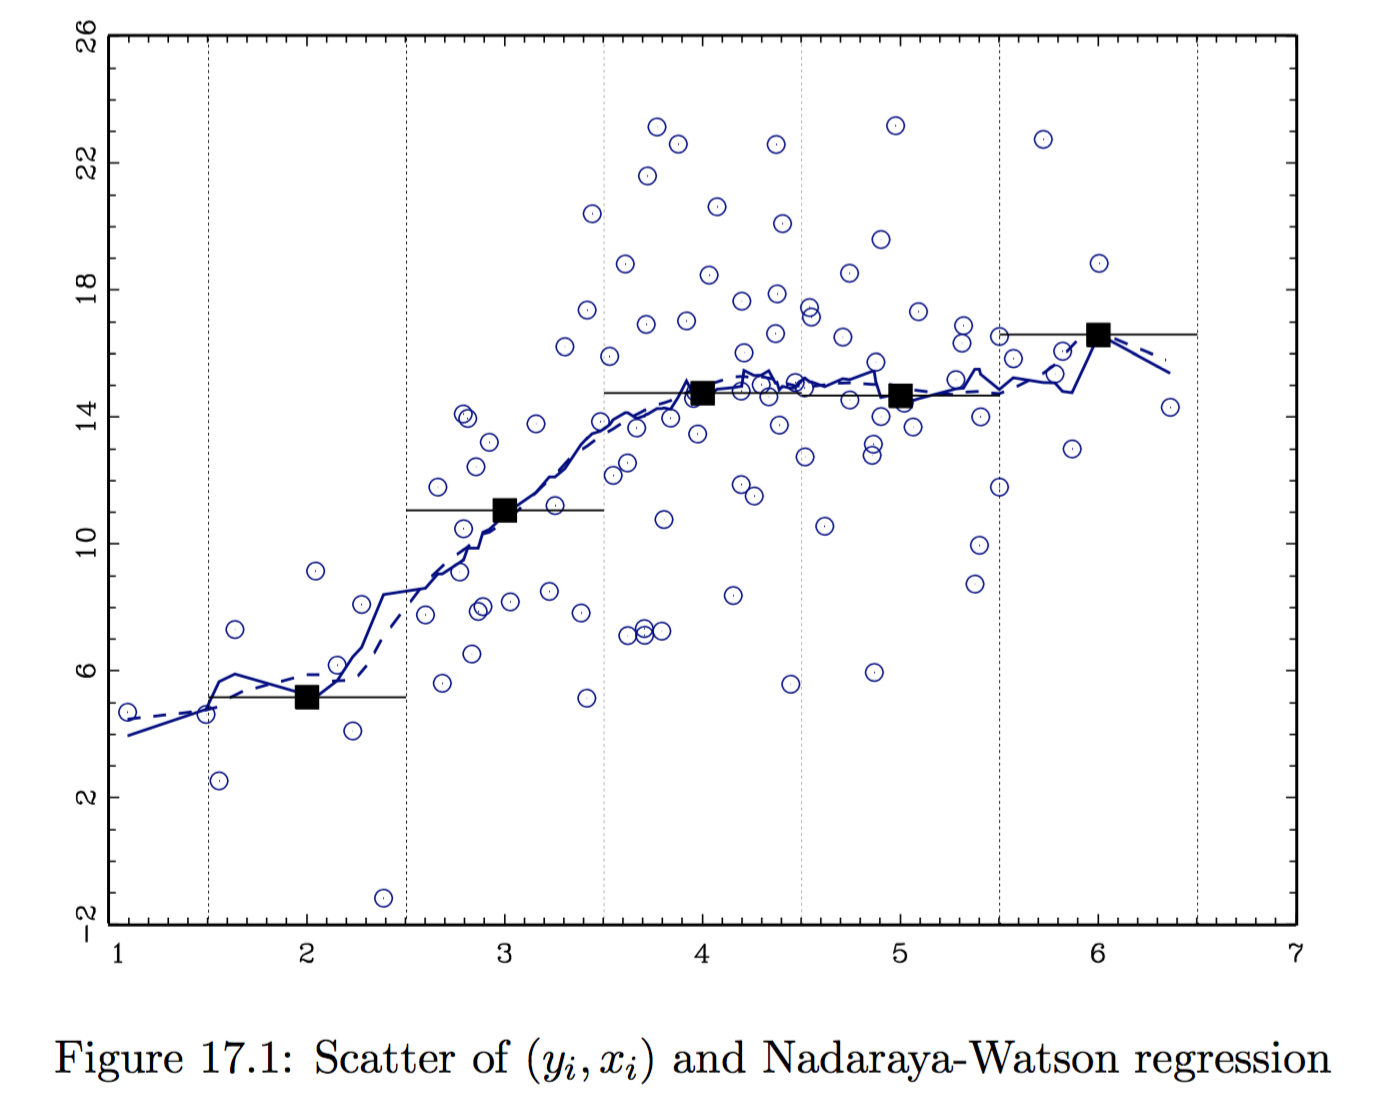
\includegraphics{figures/Fig_521.png}
\caption{NW regression}
\end{figure}

The Nadaraya-Watson estimate of the CEF takes the form:
\[
    \mathbb E_n \left[ y | x = \bar{x}\right] = \hat{g}(\bar{x}) = \frac{\sum_{i=1}^n y_i K_h (x_i - \bar{x})}{\sum_{i=1}^n K_h (x_i - \bar{x})} \\
\]

\begin{itemize}
\tightlist
\item
  \textbf{Local Linear} estimator. It assumes the CEF locally takes the form \(g(x) = \beta_0(x) + \beta_1(x) x\). The local parameters are estimated as:
  \[
  \left( \hat{\beta}_0 (\bar{x}), \hat{\beta}_1 (\bar{x}) \right) = \arg\min_{\beta_0, \beta_1}  \quad   \mathbb E_n \Big[ K_h (x_i - \bar{x}) \cdot  \big(y_i - \beta_0 - (x_i - \bar{x}) \beta_1 \big)^2 \Big]
  \]
\end{itemize}

\begin{figure}
\centering
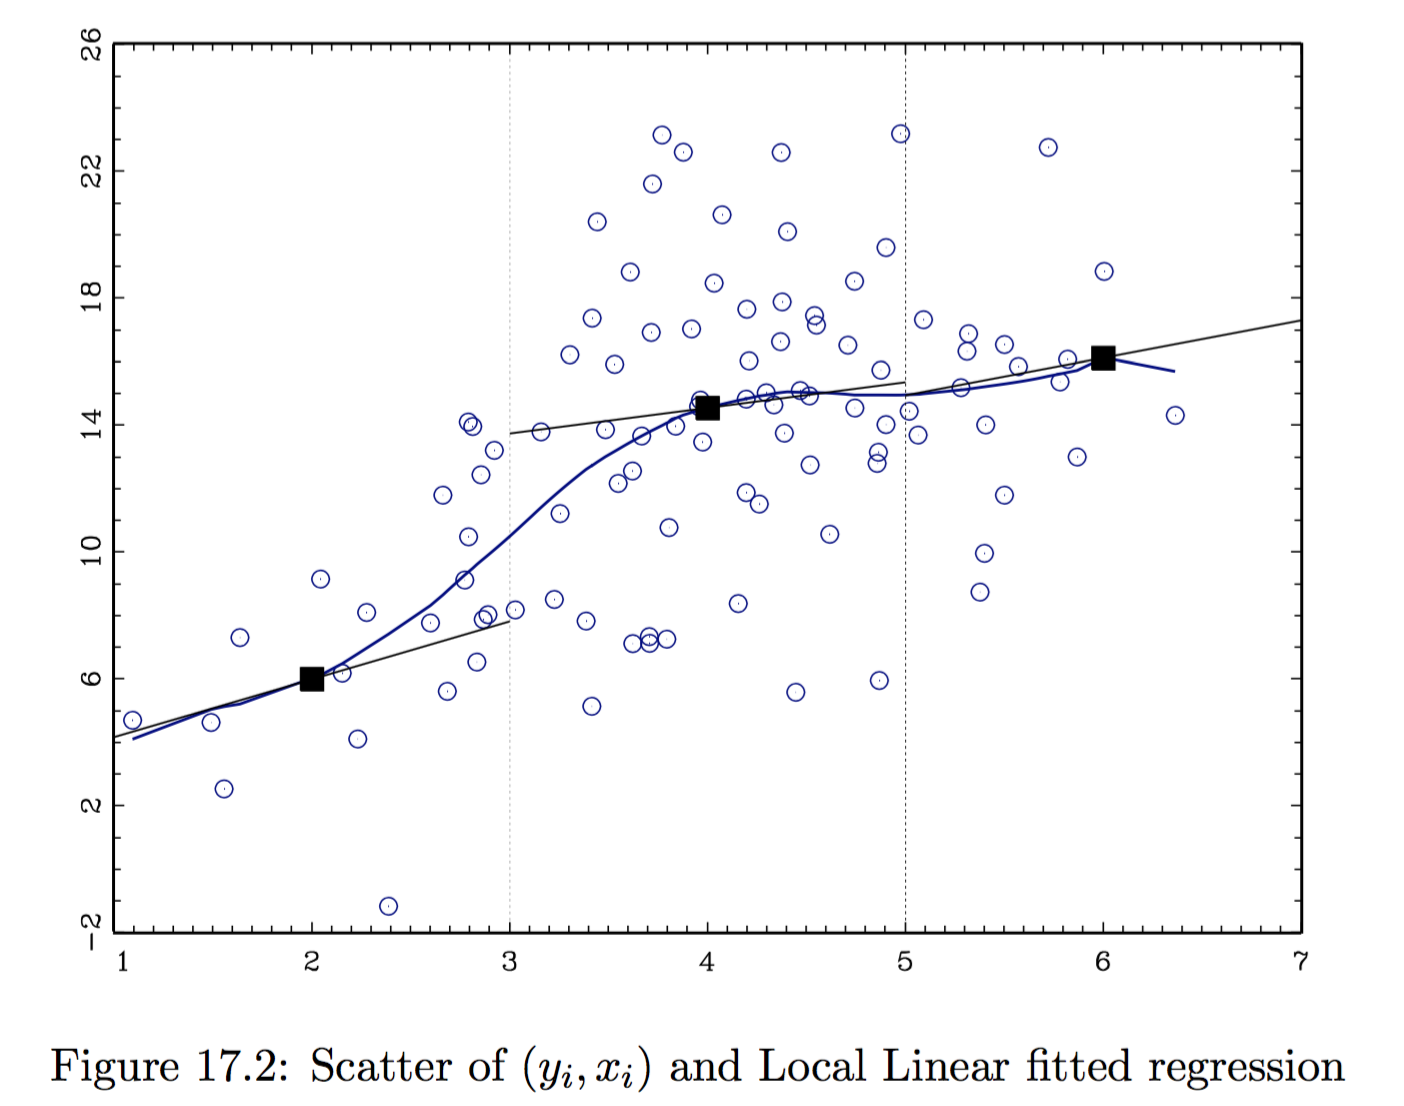
\includegraphics{figures/Fig_522.png}
\caption{LL regression}
\end{figure}

In this case, we do LS estimate with \(i\)'s contribution of residual weighted by the kernel \(K_h (x_i - \bar{x})\). The final estimate at \(\bar{x}\) is given by:
\[
  \hat{g} (\bar{x}) = \hat{\beta}_0 (\bar{x}) + (\bar{x} - \bar{x}) \hat{\beta}_1 (\bar{x}) = \hat{\beta}_0 (\bar{x})
\]
since we have centered the \(x_s\) at \(\bar{x}\) in the kernel.
- It is possible to add linearly higher order polynomials, e.g.~do locally quadratic least squares using loss function:

\[
  \mathbb E_n \left[ K_h (x_i - \bar{x}) \big(y_i - \beta_0 - (x_i - \bar{x}) \beta_1 - (x_i - \bar{x})^2 \beta_2 \big)^2 \right] 
\]

\hypertarget{kernel-examples}{%
\subsection{Kernel examples:}\label{kernel-examples}}

\begin{itemize}
\tightlist
\item
  \textbf{Uniform kernel}. LS restricted to sample \(i\) such that \(x_i\) within \(h\) of \(\bar{x}\).
  \[
  \begin{aligned}
  & K (\cdot) = \mathbb I\{ \cdot \in [-1, 1] \}  \\
  & K_h (\cdot) = \mathbb I\{ \cdot/h \in [-1, 1] \} = \mathbb I\{ \cdot \in [-h, h] \}  \\
  & K_h (x_i - \bar{x}) = \mathbb I\{ x_i - \bar{x} \in [-h, h] \}  = \mathbb I\{ x_i \in [\bar{x}-h, \bar{x} + h] \} 
  \end{aligned}
  \]
  Employed together with the locally linear estimator, the estimation procedure reduces to **local least squares\}. The loss function is:
  \[
  \mathbb E_n \Big[ K_n (x_i - \bar{x}) \big(y_i -\beta_0 - \beta_1 (x_i - \bar{x}) \big)^2 \Big] = \frac{1}{n} \sum_{i: x_i \in [\bar{x}-h, \bar{x} +h ]}  \big(y_i -\beta_0 - \beta_1 (x_i - \bar{x}) \big)^2
  \]
\end{itemize}

The more local is the estimation, the more appropriate the linear regression: if \(g_0\) is smooth, \(g_0(\bar{x}) + g_0'(\bar{x}) (x_i - \bar{x})\) is a better approximation for \(g_0 (x_i)\).

However, the uniform density is not a good kernel choice as it produces discontinuous CEF estimates. The following are two popular alternative choices that produce continuous CEF estimates.

\begin{itemize}
\item
  \textbf{Epanechnikov kernel}
  \[
    K_h(x_i - \bar{x}) = \frac { 3 } { 4 } \left( 1 - (x_i - \bar{x}) ^ { 2 } \right)  \mathbb I\{ x_i \in [\bar{x}-h, \bar{x} + h] \} 
  \]
\item
  \textbf{Normal or Gaussian kernel}
  \[
    K_\phi (x_i - \bar{x})  = \frac { 1 } { \sqrt { 2 \pi } } \exp \left( - \frac { (x_i - \bar{x}) ^ { 2 } } { 2 } \right)
  \]
\end{itemize}

\begin{figure}
\centering
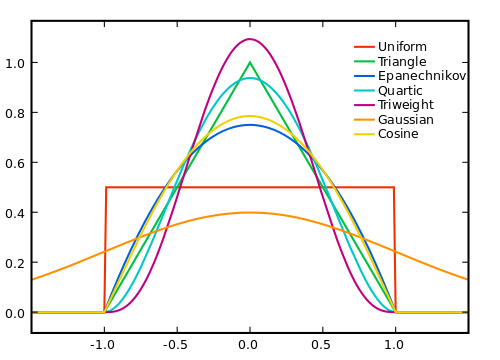
\includegraphics{figures/Fig_523.png}
\caption{Kernelsh}
\end{figure}

\begin{itemize}
\tightlist
\item
  \textbf{K-Nearest Neighbors (KNN)}: choose bandwidth so that there is a fixed number of observations in each kernel. This kernel is different from the others since it takes a nonparamentric form.
\end{itemize}

\hypertarget{choice-of-the-optimal-bandwidth}{%
\subsection{Choice of the optimal bandwidth}\label{choice-of-the-optimal-bandwidth}}

Practical methods:

\begin{itemize}
\item
  \textbf{Eyeball Method.} (i) Choose a bandwidth (ii) Estimate the regression function (iii) Look at the result: if it looks more wiggly than you would like, increase the bandwidth: if it looks more smooth than you would like, decrease the bandwidth. Con: It only works for \(\dim(x_i) = 1\) or \(2\).
\item
  \textbf{Rule of Thumb.} For example, Silverman's rule of thumb: \(h = \left( \frac{4 \hat{\sigma}^5}{3n} \right)^{\frac{1}{5}}\).
  Con: It requires too much knowledge about \(g_0\) (i.e.~normality) which you don't have.
\item
  \textbf{Cross Validation.} Under some assumptions, CV will approximately gives the MSE optimal bandwidth. The basic idea is to evaluate quality of the bandwidth by looking at how well the resulting estimator forecasts in the given sample.
\end{itemize}

Leave-one-out CV. For each \(h > 0\) and each \(i\), \(\hat{g}_{-i} (x_i)\) is the estimate of the conditional expectation at \(x_i\) using bandwidth \(h\) and all observations expect observation \(i\). The CV bandwidth is defined as
\[
    \hat{h} = \arg \min_h CV(h) = \arg \min_h \sum_{i=1}^n  \Big( y_i -  \hat{g}_{-i} (x_i) \Big)^2
\]

\begin{quote}
How to choose the optimal bandwidth:

\begin{itemize}
\tightlist
\item
  Select a value for \(h\).
\item
  For each observation \(i\), calculate
  \[
  \hat{g}_{-i} (x_i) = \frac{\sum_{j \ne i} y_j K_h (x_j - x_i) }{\sum_{i=1}^n K_h (x_j - x_i)}, \qquad e_{i,h}^2 = \left(y_i - \hat{g}_{-i} (x_i) \right)^2
  \]
\item
  Calculate \(\text{CV}(h) = \sum_{i=1}^n e^2_{i,h}\).
\item
  Repeat for each \(h\) and choose the one that minimizes \(\text{CV}(h)\).
\end{itemize}
\end{quote}

\begin{figure}
\centering
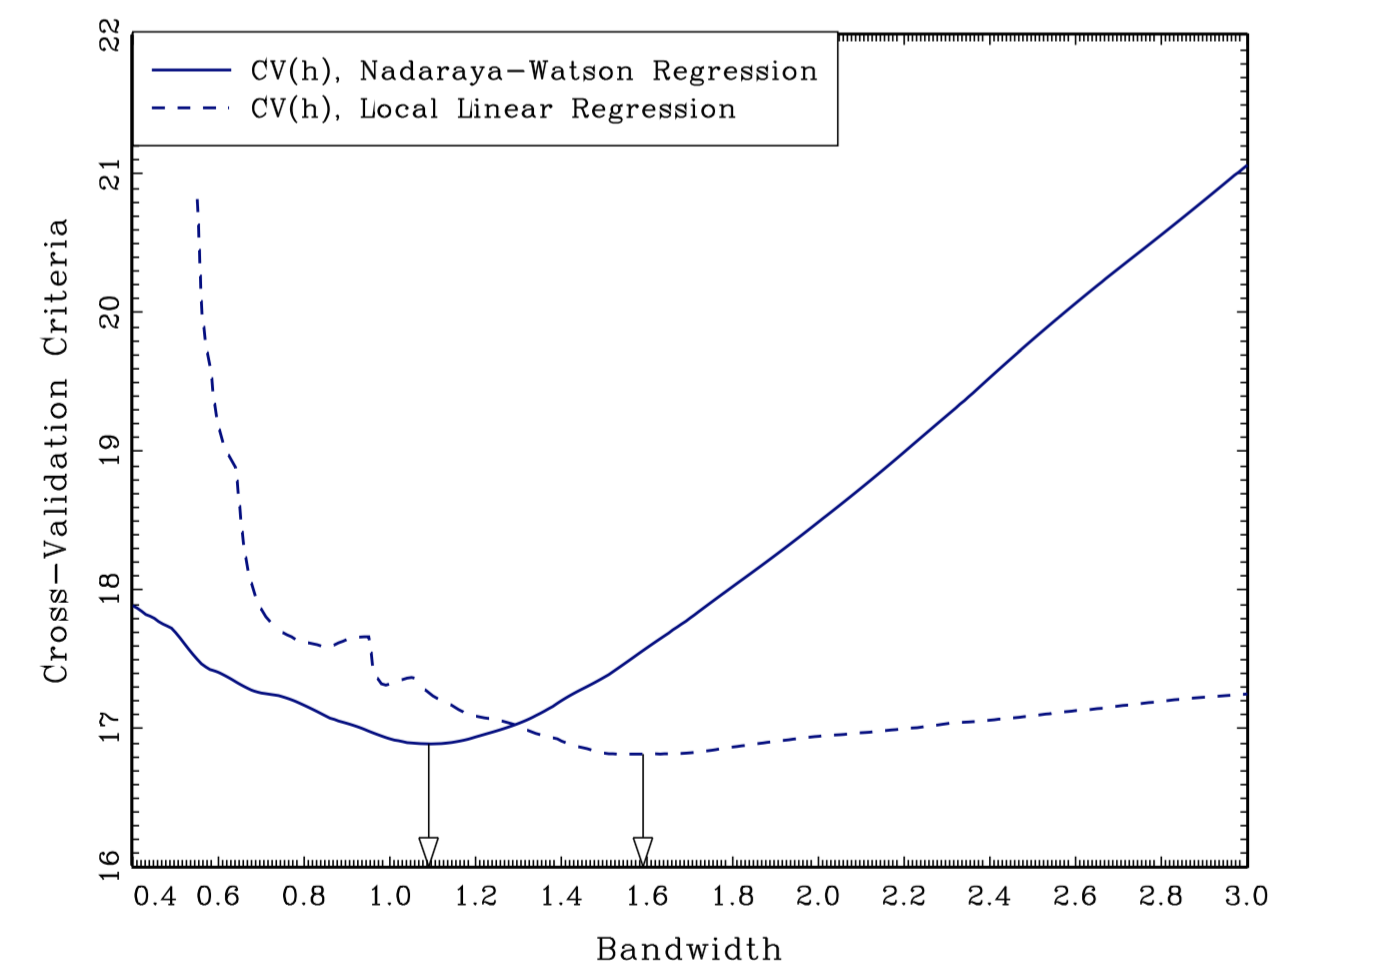
\includegraphics{figures/Fig_524.png}
\caption{Optimal Bandwidth}
\end{figure}

\hypertarget{inference-1}{%
\subsection{Inference}\label{inference-1}}

\textbf{Theorem}:
Consider data \(\{ y_i, x_i \}_{i=1}^n\), iid and suppose that \(y_i = g(x_i) + \varepsilon_i\) where \(\mathbb E[\varepsilon_i|x_i] = 0\). Assume that \(x_i \in Interior(X)\) where \(X \subseteq \mathbb R\), \(g(x)\) and \(f(x)\) are three times continuously differentiable, and \(f(x) > 0\) on \(X\). \(f(x)\) is the probability density of \(x \in X\) , and \(g(x)\) is the function of interest. Suppose that \(K(\cdot)\) is a kernel function. Suppose \(n\to\infty\), \(h\to0\) , \(nh\to\infty\), and \(nh^7\to0\). Then for any fixed \(x\in X\),
\[
  AMSE = \sqrt{nh} \Big( \hat{g}(x) - g(x) - h^2 B(x)\Big) \overset{d}{\to} N \left( 0, \frac{\kappa \sigma^2(x)}{f(x)}\right)
\]
for \(\sigma^2(x) = Var(y_i|x_i = x)\), \(\kappa = \int K^2(v)dv\), and \(B(x) = \frac{\kappa_2}{2} \frac{f'(x)g'(x) + f(x) g''(x)}{f(x)}\) where \(\kappa_2 = \int v^2 K(v)dv\).

\begin{quote}
Remark on the theorem:

\begin{itemize}
\tightlist
\item
  If the function is smooth enough and the bandwidth small enough, you can ignore the bias relative to sampling variation. To make this plausible, use a smaller bandwidth than would be the ``optimal''.
\item
  All kernel regression estimators can be written as a weighted average
  \[
  \hat{g}(x) = \frac{1}{n} \sum_{i=1}^n w_i (x) y_i, \quad \text{ with } \quad w_i (x) = \frac{n K_h (x_i - x)}{\sum_{i=1}^n K_h (x_i - x)} 
  \]
  Do inference as if you were estimating a mean \(\mathbb E[z_i]\) with sample mean \(\frac{1}{n} \sum_{i=1}^n z_i\) using \(z_i = w_i (x) y_i\).
\item
  If you are doing inference at more than one value of \(x\), do inference as in the previous point, treating each value of \(x\) as a different sample mean and note that even with independent data, these means will be correlated in general because there will generally be some common observations in to each of the averages. If you have a time series, make sure you account for correlation between the observations going in the different averages even if they don't overlap.
\end{itemize}
\end{quote}

Issue when doing inference: the estimation of the bandwidth from the data is generally not accounted for in the distributional approximation (when doing inference). In large-samples, this is unlikely to lead to large changes, but uncertainty is understated in small samples.

\hypertarget{bias-variance-trade-off}{%
\subsection{Bias-variance trade-off}\label{bias-variance-trade-off}}

\textbf{Theorem}:
For any estimator mean-square error MSE is decomposable into variance and bias-squared:
\[
\text{MSE} (\bar{x}, \hat{g}) = \mathbb E \left[ \left( \hat{g}(\bar{x}) - g_0 (\bar{x}) \right)^2 \right] = \mathbb E \Big[\underbrace{ \hat{g}(\bar{x}) - g_0 (\bar{x}) }_{\text{Bias}} \Big]^2 +  Var (\hat{g} (\bar{x})). 
\]

The theorem follows from the following corollary.

\textbf{Corollary}:
Let \(A\) be a random variable and \(\theta_0\) a fixed parameter. Then,
\[
    \mathbb E [ (A - \theta_0)^2] = Var (A) + \mathbb E [A-\theta_0]^2
\]

\textbf{Proof}:
\[
  \begin{aligned}
    \mathbb E [ (A - \theta_0)^2] & = \mathbb E[A^2] - 2 \mathbb E [A \theta_0] + \mathbb E [\theta_0] \\
    &  = \mathbb E[A^2] \underbrace{-  \mathbb E[A]^2 + E[A]^2}_{\text{add and subtract}} - 2 \mathbb E [A \theta_0] + \mathbb E [\theta_0] \\
    &  = Var(A) + \mathbb E [A]^2 - 2 \theta_0 \mathbb E [A ] + \mathbb E [\theta_0] \\
    & = Var(A) + \mathbb E [A - \theta_0]^2
    \end{aligned}
\]

Note that \(\mathbb E [ (A - \theta_0)^2] = \mathbb E [A - \theta_0]^2\).
\[\tag*{$\blacksquare$}\]

\textbf{Criteria to solve the bias-variance trade-off}:

\begin{itemize}
\item
  \textbf{Mean squared error (MSE)\}:
  \[
    \text{MSE} (\bar{x}) (\hat{g}) = \mathbb E \left[ \left( \hat{g}(\bar{x}) - g_0 (\bar{x}) \right)^2 \right] 
  \]
  }NB!** This is the criterium we are going to use.
\item
  \textbf{Integrated mean squared error (IMSE)}:
  \[
    \text{IMSE} ( \hat{g} ) = \mathbb E \left[ \int | \hat{g} (x) - g_0 (x) |^2 \mathrm{d} F(x)  \right] 
  \]
\item
  Type I - Type II error.
\end{itemize}

Hansen (2019): the theorem above implies that we can asymptotically approximate the MSE as
\[
\text{AMSE} = \Big( h^2 \sigma_k^2 B(x) \Big)^2 + \frac{\kappa \sigma^2(x)}{nh f(x)} \approx \text{const} \cdot \left( h^4 + \frac{1}{n h} \right) 
\]

Where

\begin{itemize}
\tightlist
\item
  \(Var \propto \frac{1}{h n}\), where you can think of \(n h\) as the \textbf{effective sample size}.
\item
  Bias \(\propto h^2\), derived if \(g_0\) is twice continuously differentiable using Taylor expansion.
\end{itemize}

Trade-off: the asymptotic MSE is dominated by the larger of \(h^4\) and \(\frac{1}{h n}\). Notice that the bias is increasing in \(h\) and the variance is decreasing in \(h\) (more smoothing means more observations are used for local estimation: this increases the bias but decreases estimation variance). To select \(h\) to minimize the asymptotic MSE, these two components should balance each other:
\[
\frac{1}{h n} \propto h^4 \quad \Rightarrow \quad  h \propto n^{-1/5} 
\]

This result means that the bandwidth should take the form \(h = c \cdot n^{-1/5}\). The optimal constant \(c\) depends on the kernel \(k\) the bias function \(B(x)\) and the marginal density \(f_x(x)\). A common misinterpretation is to set \(h = n^{-1/5}\) which is equivalent to setting \(c = 1\) and is completely arbitrary. Instead, an empirical bandwidth selection rule such as cross-validation should be used in practice.

\hypertarget{global-non-parametric-estimation---series}{%
\section{Global Non-Parametric Estimation - Series}\label{global-non-parametric-estimation---series}}

The goal is to try to globally approximate the CEF with a function \(g(x)\). Series methods are based on the **Stone-Weierstrass theorem\}: a real-valued continuous function \(g(x)\) defined in a compact set can be approximated with polynomials for any degree of accuracy
\[
    g_0 (x) = p_1 (x) \beta _1 + \dots + p_K (x) \beta_K + r(x)
\]
where \(p_1(x), \dots, p_K(x)\) are called ``a dictionary of approximating series'' and \(r(x)\) is a remainder function. If \(p_1(x), \dots, p_K(x)\) are sufficiently rich, \(r(x)\) will be small. If \(K \to \infty\), then \(r \to 0\).

\begin{quote}
Example - Taylor series: if \(g(x)\) is infinitely differentiable, then
\[
g(x) = \sum_{k=0}^{\infty } a_k x^k
\]
where \(a_k = \frac{1}{k!} \frac{\partial^k g_0}{\partial x^k}\).
\end{quote}

The basic idea is to approximate the infinite sum by chopping it off after \(K\) terms and then estimate the coefficients by OLS.

\textbf{Series estimation}:

\begin{itemize}
\tightlist
\item
  Choose \(K\), i.e.~the number of series terms, and an approximating dictionary \(p_1(x), \dots, p_K(x)\)
\item
  Expand data to \(D = \left( y_i, p_1(x_i), \dots, p_K(x_i) \right)_{i=1}^n\)
\item
  Estimate OLS to get \(\hat{\beta}_1, \dots, \hat{\beta}_K\)
\item
  Set \(\hat{g}(x) = p_1 (x)\hat{\beta}_1 + \dots + p_K(x) \hat{\beta}_K\)
\end{itemize}

\hypertarget{examples}{%
\subsection{Examples}\label{examples}}

\begin{itemize}
\item
  \textbf{Monomials}: \(p_1(x) = 1, p_2(x) = x, p_3(x)=x^2, \dots\)
\item
  \textbf{Hermite Polynomials}: \(p_1(x) = 1\), \(p_2(x) = x\), \(p_3(x)=x^2 -1\), \(p_4(x)= x^3 - 3x, \dots\). Con: \textbf{edge effects}. The estimated function is particularly volatile at the edges of the sample space (Gibbs effect)
\end{itemize}

\begin{figure}
\centering
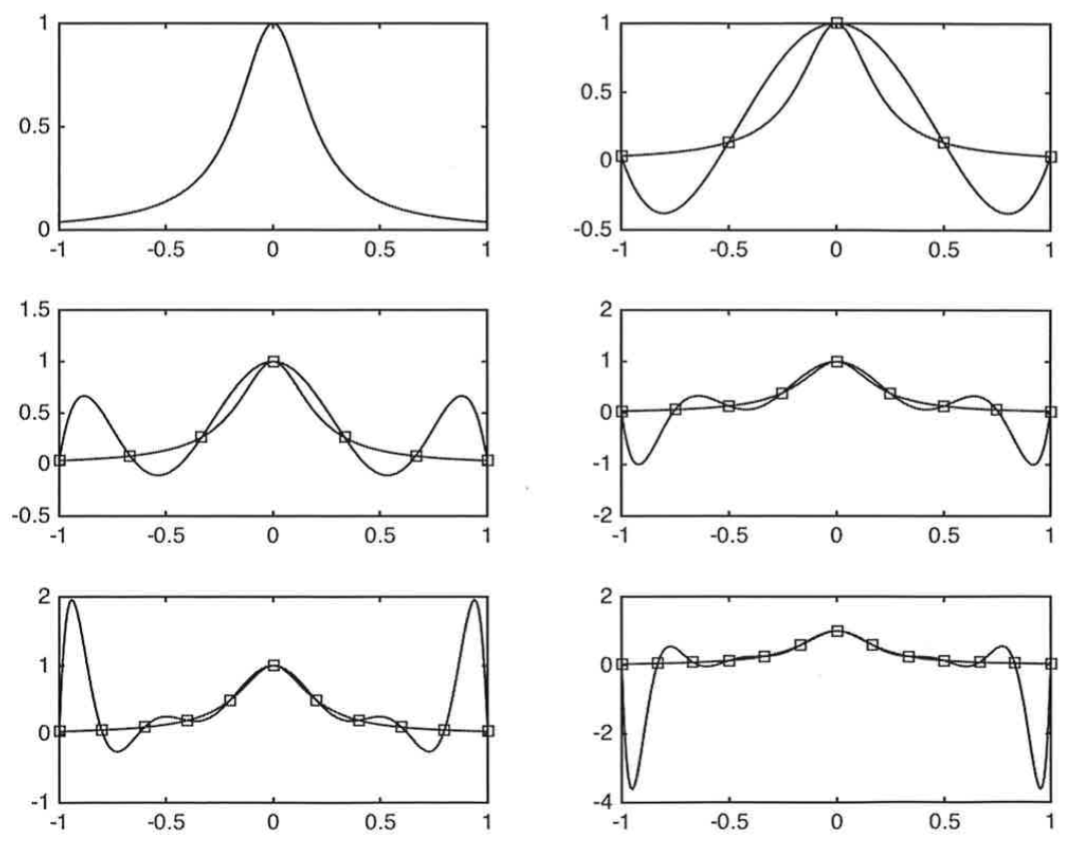
\includegraphics{figures/Fig_531.png}
\caption{Hermite Polynomials}
\end{figure}

\begin{itemize}
\item
  \textbf{Trig Polynomials}: \(p_1(x) = 1\), \(p_2(x) = \cos 2 \pi x\), \(p_3(x)= \sin 2 \pi x\), \(p_4(x) = \cos 2 \pi x \cdot 2 x \dots\). Pro: cyclical therefore good for series. Con: edge effects
\item
  \textbf{B-splines}: recursively constructed using knot points
  \[
  B_{i, 0} = \begin{cases}
  1 & \text{if } t_i \leq x < t_{i+1} \\ 0 & \text{otherwise}
  \end{cases} \qquad B_{i_k} (x) = \frac{x - t_i}{ t_{i+k} - t_i} B_{i, k-1} (x) +  \frac{t_{i+k+1}-x}{t_{i+k+1} - t_{i+1}} B_{i+1, k-1} (x)
  \]
  where \(t_0, \dots, t_i, \dots\) are knot points and \(k\) is the order of the spline.
  Pro: faster rate of convergence and lower asymptotic bias.
\end{itemize}

\hypertarget{estimation}{%
\subsection{Estimation}\label{estimation}}

Given \(K\), inference proceeds exactly as if one had run an OLS of \(y\) on \((p_k)_{k=1}^K\). The idea is that you ignore that you are doing non-parametric regression as long as you believe you have put enough terms (high \(K\)). Then the function is smooth enough so that the bias of the approximation is small relative to the variance (see Newey, 1997). Note that his approximation does not account for data-dependent estimation of the bandwidth.

Newey (1997): results about consistency of \(\hat{g}\) and asymptotic normality of \(\hat{g}\).

\begin{itemize}
\tightlist
\item
  OLS: \(\hat{\beta} \overset{p}{\to} \beta_0\)
\item
  Non-parametric: you have a sequence \(\{\beta_k\}_{k=1}^K\) with \(\hat{\beta}_k \overset{p}{\to} \beta_k\) as \(n \to \infty\) (as \(k \to \infty\)). However, this does not make sense because \(\{\beta_k\}\) is not constant. Moreover, \(\beta_k\) is not the quantity of interest. We want to make inference on \(\hat{g}(x)\).
\end{itemize}

\textbf{Theorem}:
Under regularity conditions, including \(| | \hat{\beta} - \beta_0 | | \overset{p}{\to} 0\),

\begin{itemize}
\tightlist
\item
  Uniform Consistency: \(\sup_x | \hat{g}(x) - g_0(x)| \overset{p}{\to} 0\)
\item
  Mean-square Consistency: \(\int | \hat{g}(x) - g_0(x)|^2 \mathrm{d} F(x) \overset{p}{\to} 0\)
\end{itemize}

\textbf{Theorem}:
Under the following assumptions:

\begin{itemize}
\tightlist
\item
  \((x_i, y_i)\) are iid and \(Var(y_i|x_i)\) is bounded;
\item
  For all \(K\), there exists a non-singular matrix \(B\) such that \(A = \left[ (B p(x)) (B p(x))' \right]\) where \(p(x) = \left( p_1(x), \dots, p_K (x) \right)\) has the properties that \(\lambda_{\min} (A)^{-1} = O(1)\). In addition, \(\sup_x | | B p(x) | | = o(\sqrt{K/n})\).
\item
  There exists \(\alpha\) and \(\beta_K\) for all \(K\) such that
  \[
    \sup_x | g_0 (x) - p(x) \beta_K | = O_p(K^{-\alpha})
  \]
\end{itemize}

Then, it holds that

\[
  \text{IMSE = }\int \left( g_0 (x) - \hat{g} (x) \right)^2 \mathrm{d} F(x) = O_p \left( \frac{K}{n} + K^{-2\alpha}\right)
\]

\hypertarget{choice-of-the-optimal-k}{%
\subsection{\texorpdfstring{Choice of the optimal \(K\)}{Choice of the optimal K}}\label{choice-of-the-optimal-k}}

The bias-variance trade-off for series comes in through the choice of \(K\):

\begin{itemize}
\tightlist
\item
  Higher \(K\): smaller bias, since we are leaving out less terms form the infinite sum.
\item
  Smaller \(K\): smaller variance, since we are estimating less regression coefficients from the same amount of data.
\end{itemize}

\textbf{Cross-validation for series}:
For each \(K \geq 0\) and for each \(i=1, \dots, n\), consider

\[
  D_{-i} = \{ (x_1, y_1), \dots, (x_{i-1}, y_{i-1}),(x_{i+1}, y_{i+1}), \dots (x_n, y_n) \}
\]
and calculate \(\hat{g}^{(K)}_{-i} (x)\) using series estimate with \(p_1(x), \dots, p_K (x)\) in order to get \(e^{(K)}_i = y_i - \hat{g}^{(K)}_{-i} (x_i)\). Choose \(\hat{K}\) such that

\[
  \hat{K} = \arg \min_K \mathbb E_n \left[ {e^{(K)}_i}^2 \right]
\]

\hypertarget{inference-2}{%
\subsection{Inference}\label{inference-2}}

Consider the data \(D = \{ (x_i, y_i) \}_{i=1}^n\) such that \(y_i = g_0 (x_i) + \varepsilon_i\). You may want to form confidence intervals for quantities that depends on \(g_0\).

\begin{quote}
Example: \(\theta_0\) functional forms of interests:

\begin{itemize}
\tightlist
\item
  Point estimate: \(\theta_0 = g_0 (\bar{x} )\) for fixed \(\bar{x}\)
\item
  Interval estimate: \(\theta_0 = g_0 (\bar{x}_2) - g_0 (\bar{x}_1)\)
\item
  Point derivative estimate: \(\theta_0 = g_0 ' (\bar{x})\) at \(\bar{x}\)
\item
  Average derivative \(\theta_0 = \mathbb E [g_0 ' (x) ]\)
\item
  Consumer surplus: \(\theta_0 = \int_a^b g_0(x)dx \quad\) when \(g_0\) is a demand function.
\end{itemize}
\end{quote}

Those estimates are functionals: maps from a function to a real number. We are doing inference on a function now, not on a point estimate.

In order to form a confidence interval for \(\theta_0\), with series you can

\begin{itemize}
\tightlist
\item
  \textbf{Undersmooth}: in order to apply a \textit{central limit theorem}, you need deviations around the function to be approximately gaussian. Undersmoothing makes the function oscillate much more than the curve you are estimating in order to obtain such guassian deviations.
\end{itemize}

\begin{figure}
\centering
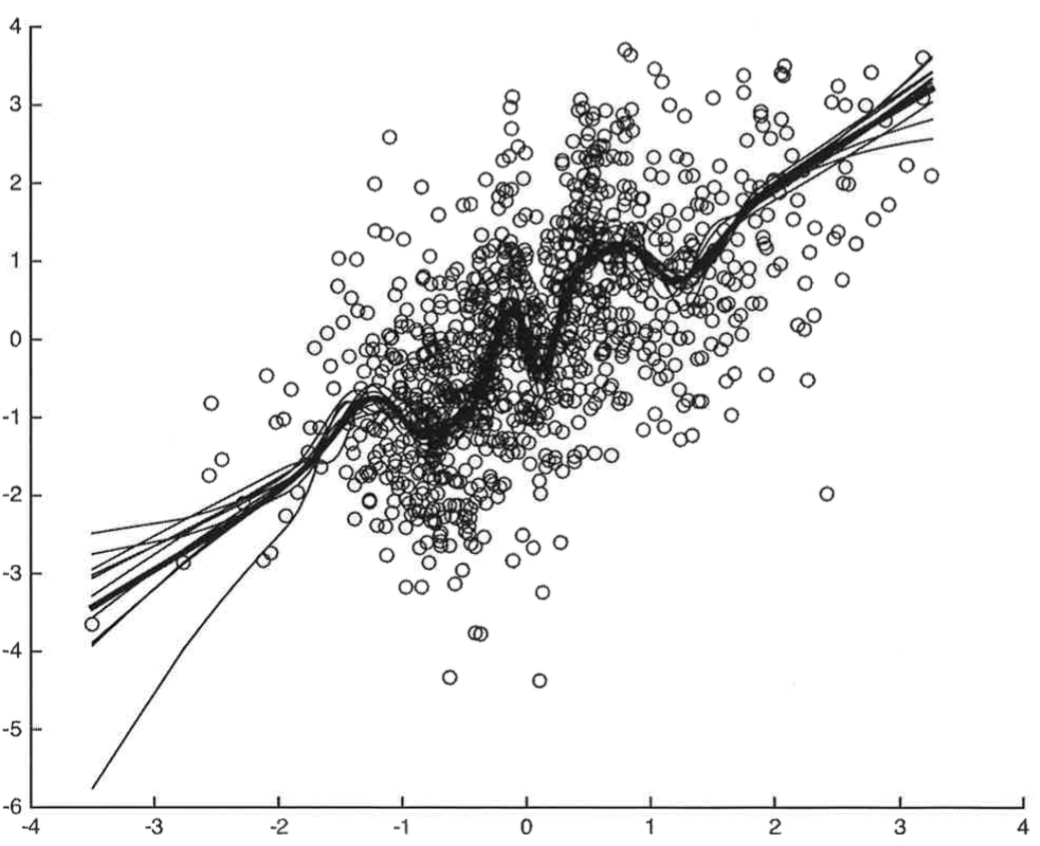
\includegraphics{figures/Fig_541.png}
\caption{Smoothing}
\end{figure}

\begin{quote}
Example: if on the contrary you oversmooth (e.g.~\(g_0\) linear), errors are going to constantly be on either one or the other side of the curve \(\to\) not gaussian!
\end{quote}

\begin{itemize}
\tightlist
\item
  Use the \textbf{delta method}. It would usually require more series terms than a criterion like cross-validation would suggest.
\end{itemize}

\textbf{Theorem}:
Under the assumptions of the consistency theorem
\[
    \frac{\sqrt{n} \Big(\hat{\theta} - \theta_0 + B(r_K) \Big)}{\sqrt{v_K}} \overset{d}{\to} N (0,1)
\]

\textbf{Theorem}:
Under the assumptions of the consistency theorem and \(\sqrt{n} K^{-\alpha} = o(1)\) (or equivalently \(n K^{-2\alpha} = O(1)\) in Hansen),
\[
  \frac{\sqrt{n} \Big(\hat{\theta} - \theta_0 \Big)}{\sqrt{v_K}} \overset{d}{\to} N (0,1)
\]

\begin{quote}
Remark on convergence rate:

\begin{itemize}
\tightlist
\item
  The rate of convergence of splines is faster than for power series (Newey 1997).
\item
  We have **undersmoothing\} if \(\sqrt{n} K^{\alpha} = o(1)\) (see comment below)
\item
  Usually, in order to prove asymptotic normality, we first prove unbiasedness. However here we have a \textbf{biased} estimator but we make the bias converge to zero faster than the variance.
\end{itemize}
\end{quote}

Hansen (2019): The critical condition is the assumption that \(\sqrt{n} K^{\alpha} = o(1)\) This requires that \(K \to \infty\) at a rate faster than \(n^{\frac{1}{2\alpha}}\) This is a troubling condition. The optimal rate for estimation of \(g(x)\) is \(K = O(n^{\frac{1}{1+ 2\alpha}})\). If we set \(K = n^{\frac{1}{1+ 2\alpha}}\) by this rule then \(n K^{-2\alpha} = n^{\frac{1}{1+ 2\alpha}} \to \infty\) not zero. Thus this assumption is equivalent to assuming that \(K\) is much larger than optimal. The reason why this trick works (that is, why the bias is negligible) is that by increasing \(K\) the asymptotic bias decreases and the asymptotic variance increases and thus the variance dominates. Because \(K\) is larger than optimal, we typically say that \(\hat{g}(x)\) is \textbf{undersmoothed} relative to the optimal series estimator.

\begin{quote}
Many authors like to focus their asymptotic theory on the assumptions in the theorem, as the distribution of \(\theta\) appears cleaner. However, it is a poor use of asymptotic theory. There are three problems with the assumption \(\sqrt{n} K^{-\alpha} = o(1)\) and the approximation of the theorem.

\begin{itemize}
\tightlist
\item
  First, it says that if we intentionally pick \(K\) to be larger than optimal, we can increase the estimation variance relative to the bias so the variance will dominate the bias. But why would we want to intentionally use an estimator which is sub-optimal?
\item
  Second, the assumption \(\sqrt{n} K^{-\alpha} = o(1)\) does not eliminate the asymptotic bias, it only makes it of lower order than the variance. So the approximation of the theorem is technically valid, but the missing asymptotic bias term is just slightly smaller in asymptotic order, and thus still relevant in finite samples.
\item
  Third, the condition \(\sqrt{n} K^{\alpha} = o(1)\) is just an assumption, it has nothing to do with actual empirical practice. Thus the difference between the two theorems is in the assumptions, not in the actual reality or in the actual empirical practice. Eliminating a nuisance (the asymptotic bias) through an assumption is a trick, not a substantive use of theory. My strong view is that the result (1) is more informative than (2). It shows that the asymptotic distribution is normal but has a non-trivial finite sample bias.
\end{itemize}
\end{quote}

\hypertarget{kernel-vs-series}{%
\subsection{Kernel vs Series}\label{kernel-vs-series}}

Hansen (2019): in this and the previous chapter we have presented two distinct methods of nonparametric regression based on kernel methods and series methods. Which should be used in practice? Both methods have advantages and disadvantages and there is no clear overall winner.

First, while the asymptotic theory of the two estimators appear quite different, they are actually rather closely related. When the regression function \(g(x)\) is twice differentiable \((s = 2)\) then the rate of convergence of both the MSE of the kernel regression estimator with optimal bandwidth \(h\) and the series estimator with optimal \(K\) is \(n^{-\frac{2}{k+4}}\) (where \(k = \dim(x)\)). There is no difference. If the regression function is smoother than twice differentiable (\(s > 2\)) then the rate of the convergence of the series estimator improves. This may appear to be an advantage for series methods, but kernel regression can also take advantage of the higher smoothness by using so-called higher-order kernels or local polynomial regression, so perhaps this advantage is not too large.

Both estimators are asymptotically normal and have straightforward asymptotic standard error formulae. The series estimators are a bit more convenient for this purpose, as classic parametric standard error formula work without amendment.

An advantage of kernel methods is that their distributional theory is easier to derive. The theory is all based on local averages which is relatively straightforward. In contrast, series theory is more challenging, dealing with increasing parameter spaces. An important difference in the theory is that for kernel estimators we have explicit representations for the bias while we only have rates for series methods. This means that plug-in methods can be used for bandwidth selection in kernel regression. However, typically we rely on cross-validation, which is equally applicable in both kernel and series regression.

Kernel methods are also relatively easy to implement when the dimension of \(x\), \(k\), is large. There is not a major change in the methodology as \(k\) increases. In contrast, series methods become quite cumbersome as \(k\) increases as the number of cross-terms increases exponentially. E.g (\(K=2\)) with \(k=1\) you have only \(\{x_1, x_1^2\}\); with \(k=2\) you have to add \(\{x_2, x_2^2, x_1 x_2 \}\); with \(k=3\) you have to add \(\{x_3, x_3^2, x_1 x_3, x_2 x_3\}\), etc..

A major advantage of series methods is that it has inherently a high degree of flexibility, and the user is able to implement shape restrictions quite easily. For example, in series estimation it is relatively simple to implement a partial linear CEF, an additively separable CEF, monotonicity, concavity or convexity. These restrictions are harder to implement in kernel regression.

\hypertarget{references-7}{%
\section{References}\label{references-7}}

\begin{itemize}
\tightlist
\item
  Newey, W. K. (1997). \emph{Convergence rates and asymptotic normality for series estimators}. Journal of Econometrics, 79(1), 147--168.
\item
  Hansen (2019). ``\emph{Econometrics}''. Chapters 19, 20 and 21.
\item
  Kozbur (2019). PhD Econometrics - Lecture Notes.
\end{itemize}

\hypertarget{lecture5}{%
\chapter{Variable Selection}\label{lecture5}}

\hypertarget{lasso}{%
\section{Lasso}\label{lasso}}

Lasso (Least Absolute Shrinkage and Selection Operator) is a popular method for high dimensional regression. It does variable selection and estimation simultaneously. It is a non-parametric (series) estimation technique part of a general class of estimators called \emph{penalized estimators}. It allows the number of regressors, \(p\), to be larger than the sample size, \(n\).

Consider data \(D = \{ x_i, y_i \}_{i=1}^n\) with \(\dim (x_i) = p\). Assume that \(p\) is large relative to \(n\). Two possible reasons:

\begin{itemize}
\tightlist
\item
  we have an intrinsic problem of high dimensionality
\item
  \(p\) indicates the number of expansion terms of small number of underlying important variables (e.g.~series estimation)
\end{itemize}

\textbf{Assumption}:
\(y_i = x_i' \beta_0 + r_i + \varepsilon_i\) where \(\beta_0\) depends on \(p\), \(r_i\) is a remainder term.

Note that in classic non-parametrics, we have \(x_i'\beta_0\) as \(p_1(x_i) \beta_{1,K} + \dots + p_K(x_i) \beta_{K,K}\). For simplicity, we assume \(r_i = 0\), as if we had extreme undersmoothing. Hence the model becomes:
\[
    y_i = x_i' \beta_0 + \varepsilon_i, \qquad p \geq n
\]
We cannot run OLS because \(p \geq n\), thus the rank condition is violated.

We define the \textbf{Lasso estimator} as
\[
    \hat{\beta}_L = \arg \min \quad \underbrace{\mathbb E_n \Big[ (y_i - x_i' \beta)^2 \Big]}_{\text{SSR term}} + \underbrace{\frac{\lambda}{n} \sum_{j=1}^{P} | \beta_j |}_{\text{Penalty term}}
\]
where \(\lambda\) is called \textbf{penalty parameter}.

The \textbf{penalty term} discourages large values of \(| \beta_j |\).
The choice of \(\lambda\) is analogous to the choice of \(K\) in series estimation and \(h\) in kernel estimation.

\begin{quote}
The shrinkage to zero of the coefficients directly follows from the \(|| \cdot ||_1\) norm. On the contrary, another famous penalized estimator, \emph{ridge regression}, uses the \(|| \cdot ||_2\) norm and does not have this property.
\end{quote}

\begin{figure}
\centering
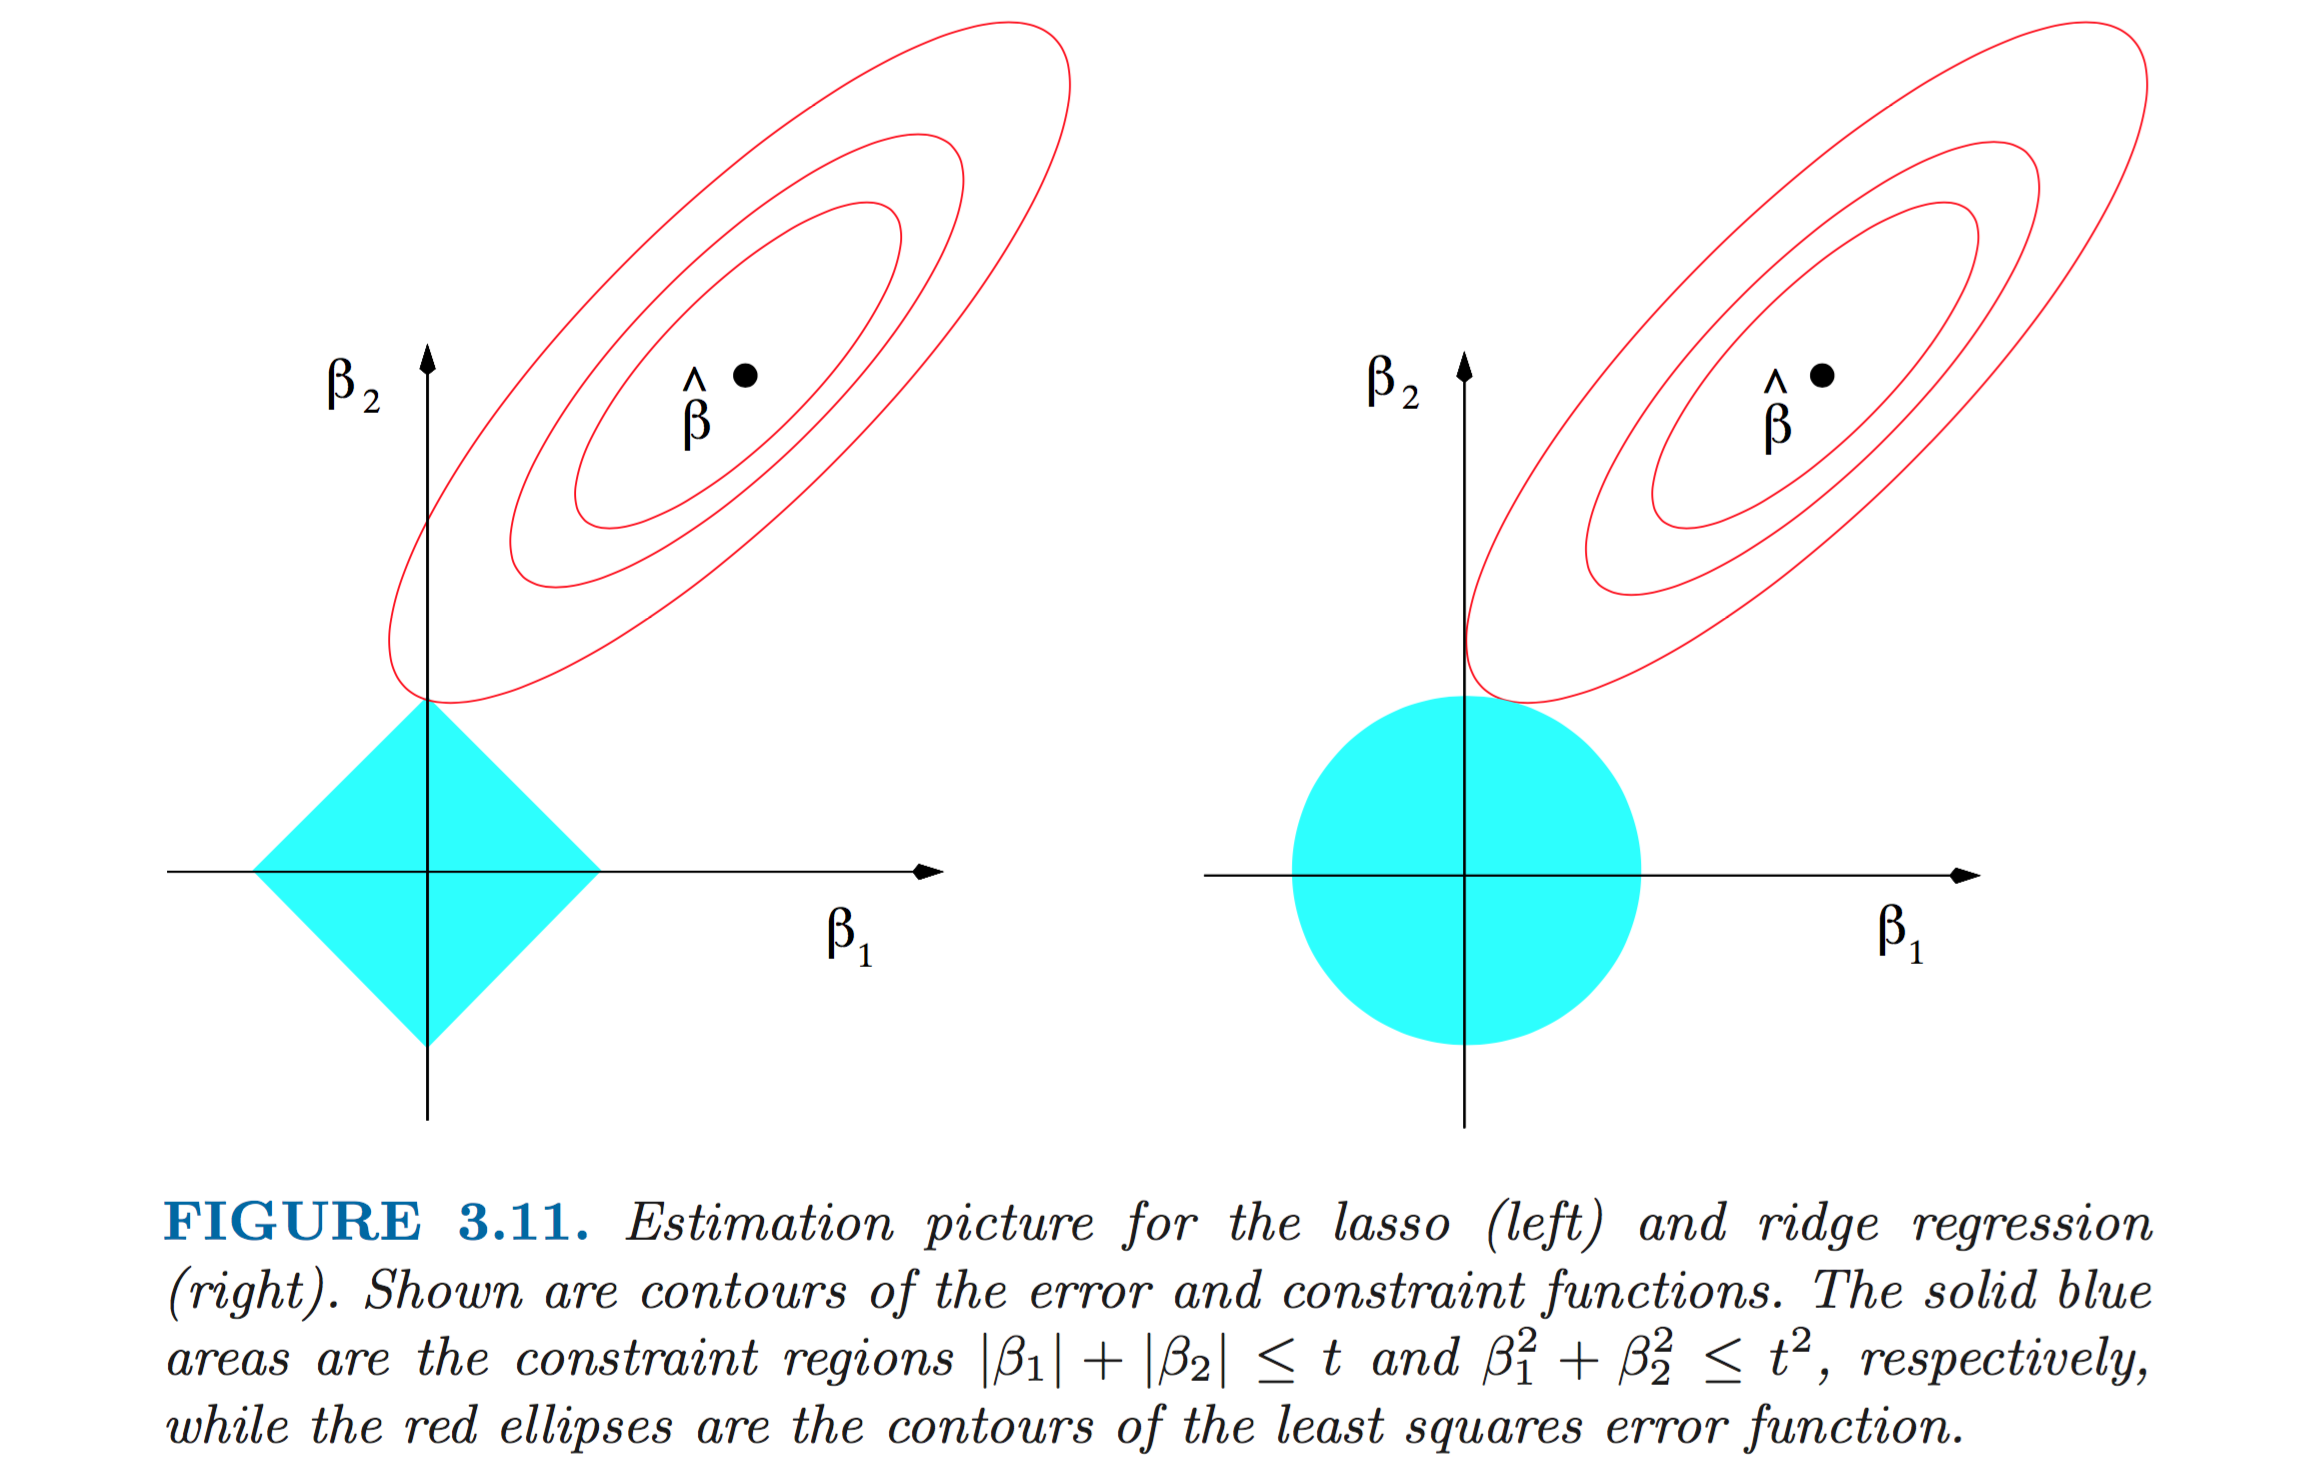
\includegraphics{figures/Fig_551.png}
\caption{Constraints}
\end{figure}

\begin{quote}
Minimizing SSR + penalty is equivalent to minimize SSR \(s.t.\) pen \(\leq c\) (clear from the picture).
\end{quote}

Let \(S_0 = \{ j: \beta_{0,j} \ne 0 \}\), we define \(s_0 = \# S_0\) as the \textbf{sparsity} of \(\beta_0\). If \(s_0/n \to 0\), we are dealing with a \textbf{sparse regression} (analogous of smooth regression).

\begin{quote}
Remark on sparsity:

\begin{itemize}
\tightlist
\item
  In words, sparsity means that even if we have a lot of variables, only a small number of them (relative to \(n\)) have an effect on the dependent variable.
\item
  \emph{Approximate sparsity imposes a restriction that only \(s_0\) variables among all of \(x_{ij}\), where \(s_0\) is much smaller than \(n\), have associated coefficients \(\beta_{0j}\) that are different from zero, while permitting a nonzero approximation error. Thus, estimators for this kind of model attempt to learn the identities of the variables with large nonzero coefficients, while simultaneously estimating these coefficients.} (Belloni et al., 2004)
\item
  Sparsity is an assumption. \(\beta_0\) is said to be \(s_0\)-sparse with \(s_0 < n\) if
  \[
  | \{ j: \beta_{0j} \neq 0 \} | \leq s_0
  \]
\end{itemize}
\end{quote}

\textbf{Theorem}:
Suppose that for data \(D_n = (y_i, x_i)_{i=1}^N\) with \(y_i = x_i' \beta + \varepsilon_i\). Let \(\hat{\beta}_L\) be the Lasso estimator. Let \(\mathcal{S} = 2 \max_j | \mathbb E[ x_{ij} \varepsilon_i] |\). Suppose \(|support(\beta_0) \leq s_0\) (sparsity assumption). Let \(c_0 = (\mathcal{S} + \lambda/n )/(-\mathcal{S} + \lambda/n )\). Let
\[
    \kappa_{c_0, s_0} = \min_{  d \in \mathbb R^p, A \subseteq \{ 1, ... , p \} : |A| \leq s_0 ,  || d_{A^c}|| \leq c_0 || d_A ||_1  }  \sqrt{  \frac{ s_0 d' \mathbb E_n [x_i x_i'] d }{|| d_A ||_1^2}  }
\]
Then

\[
    \mathbb I_{ \left\{ \frac{\lambda}{n} > \mathcal{S}  \right\}} \mathbb E_n [(x_i \beta_0 - x_i \beta_L)^2]^{\frac{1}{2}}  \leq 2 \frac{\lambda}{n} \frac{\sqrt{s_0}}{\kappa_{c_0, s_0}} \\
\]

Intuition: for a sufficiently high lambda the root mean squared error of Lasso is approximately zero.

\[
    \text{ RMSE }:  \mathbb E_n [(x_i \beta_0 - x_i \beta_L)^2]^{\frac{1}{2}}  \simeq 0  \quad \Leftrightarrow \quad \frac{\lambda}{n} > \mathcal{S}
\]

\begin{quote}
Remarks on the theorem:

\begin{itemize}
\tightlist
\item
  The minimization region is the set of ``essentially sparse'' vectors \(d \in \mathbb R^p\), where ``essentially sparse'' is defined by \(\mathcal{C}, \mathcal{S}\). In particular the condition \(k_{\mathcal{C}, \mathcal{S}}>0\) means that no essentially sparse vector \(d\) has \(\mathbb E[x_i x_i']d = 0\), i.e.~regressors were not added multiple times.
\item
  Need to dominate the score with the penalty term \(\lambda\).
\item
  Need no collinearity on a small (\(\leq s_0\)) subset of regressors (\(\to k_{c_0, s_0}>0\)).
\end{itemize}
\end{quote}

\textbf{When Lasso?} For prediction problems in high dimensional environments. \textbf{NB!} Lasso is not good for inference, only for prediction.

In particular, in econometrics it's used for selecting either

\begin{itemize}
\tightlist
\item
  instruments (predicting \(\hat{x}\) in the first stage)
\item
  control variables (next section: double prediction problem, in the first stage and in the reduced form)
\end{itemize}

\hypertarget{choosing-the-optimal-lambda}{%
\subsection{Choosing the optimal lambda}\label{choosing-the-optimal-lambda}}

The choice of \(\lambda\) determines the bias-variance tradeoff:

\begin{itemize}
\tightlist
\item
  if \(\lambda\) is too big: \(\lambda \approx \infty \mathbb \Rightarrow \hat{\beta} \approx 0\);
\item
  if \(\lambda\) is too small: \(\lambda \approx 0 \mathbb \Rightarrow\) overfitting.
\end{itemize}

Possible solutions: Bonferroni correction, bootstrapping or \(\frac{\lambda}{n} \asymp \sqrt{\frac{\log(p)}{n}}\) (asymptotically equal to), \(\mathcal{S}\) behaves like the maximum of gaussians.

\textbf{The Lasso Path}: how the estimated \(\hat{\beta}\) depends on the penalty parameter \(\lambda\)?

\begin{figure}
\centering
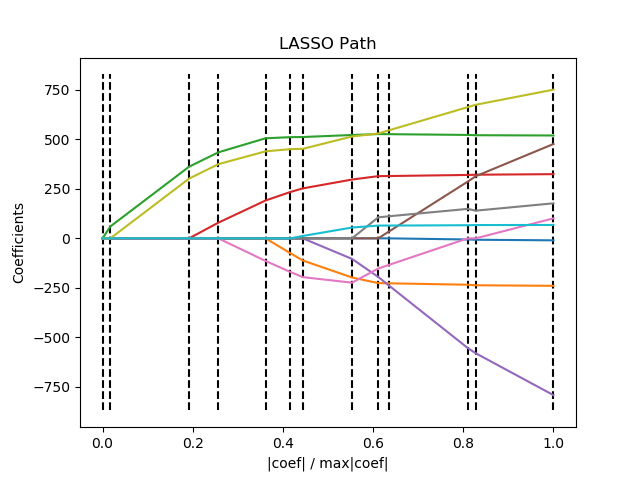
\includegraphics{figures/Fig_642.png}
\caption{Lasso Path}
\end{figure}

\textbf{Post Lasso}: fit OLS without the penalty with all the nonzero coeficients selected by Lasso in the first step.

\begin{quote}
Remarks on Lasso:

\begin{itemize}
\tightlist
\item
  Do not do inference with post-Lasso because standard errors are not uniformely valid.
\item
  As \(n \to \infty\) the CV and the \textbf{score domination} bounds converge to a unique bound.
\item
  What is the problem of cross-validation? In high dimensional settings you can overfit in so many ways that CV doesn't work and still overfits.
\item
  Using \(\lambda\) with \(\frac{\lambda}{n} > \mathcal{S}\) small coefficients get shrunk to zero with high probability. In this case with small we mean \(\propto \frac{1}{\sqrt{n}}\) or \(2 \max_j | \mathbb E_n[\varepsilon_i x_{ij}] |\).
\item
  If \(| \beta_{0j}| \leq \frac{c}{\sqrt{n}}\) for a sufficiently small constant \(c\), then \(\hat{\beta}_{LASSO} \overset{p}{\to} 0\).
\item
  In standard t-tests \(c = 1.96\).
\item
  \(\sqrt{n}\) factor is important since it is the demarcation line for reliable statistical detection.
\end{itemize}
\end{quote}

What is the criterium that should guide the selection of \(\lambda\)?
\[
  \frac{\lambda}{n} \geq 2 \mathbb E_n[x_{ij} \varepsilon_i] \qquad \forall j \quad \text{ if } Var(x_{ij} \varepsilon_i) = 1
\]

How to choose the optimal \(\lambda\):

\begin{itemize}
\tightlist
\item
  Decide the coverage of the confidence intervals (\(1-\alpha\)):
  \[
  \Pr \left( \sqrt{n} \Big| \mathbb E_n [x_{ij} \varepsilon_i] \Big| > t \right) = 1- \alpha
  \]
\item
  Solve for \(t\)
\item
  Get \(\lambda\) such that all scores are dominated by \(\frac{\lambda}{n}\) with \(\alpha\%\) probability.
\end{itemize}

\begin{quote}
It turns out that the optimal \(t \propto \sqrt{\log(p)}\)
\end{quote}

\hypertarget{pre-testing}{%
\section{Pre-Testing}\label{pre-testing}}

Main reference for this section: Belloni, Chernozhukov and Hansen \emph{Inference for Treatment Effects with High Dimensional Controls} in the \emph{Review of Economic Studies} (2014).

\hypertarget{omitted-variable-bias}{%
\subsection{Omitted Variable Bias}\label{omitted-variable-bias}}

Consider two separate statistical models. Assume the following \textbf{long regression} of interest:

\[
  y_i = x_i' \alpha_0+ z_i' \beta_0 + \varepsilon_i
\]

Define the corresponding \textbf{short regression} as

\[
  y_i = x_i' \alpha_0 + v_i \quad \text{ with } v_i = z_i' \beta_0 + \varepsilon_i
\]

\textbf{Theorem}:
Suppose that the DGP for the long regression corresponds to \(\alpha_0\), \(\beta_0\). Suppose further that \(\mathbb E[x_i] = 0\), \(\mathbb E[z_i] = 0\), \(\mathbb E[\varepsilon_i |x_i,z_i] = 0\). Then, unless \(\beta_0 = 0\) or \(z_i\) is orthogonal to \(x_i\), the (sole) stochastic regressor \(x_i\) is correlated with the error term in the short regression which implies that the OLS estimator of the short regression is inconsistent for \(\alpha_0\) due to the omitted variable bias. In particular, one can show that the plim of the OLS estimator of \(\hat{\alpha}_{SHORT}\) from the short regression is
\[
    \hat{\alpha}_{SHORT} \overset{p}{\to} \frac{Cov(y_i, x_i)}{Var(x_i)} = \alpha_0 + \beta_0 \frac{Cov(z_i, x_i)}{Var(x_i)}
\]

\hypertarget{pre-test-bias}{%
\subsection{Pre-test bias}\label{pre-test-bias}}

Consider data \(D= (y_i, x_i, z_i)_{i=1}^n\), where the true model is:
\[
\begin{aligned}
& y_i = x_i' \alpha_0  + z_i' \beta_0 + \varepsilon_i \\
& x_i = z_i' \gamma_0 + u_i
\end{aligned}
\]

Where \(x_i\) is the variable of interest (we want to make inference on \(\alpha_0\)) and \(z_i\) is a high dimensional set of control variables.

From now on, we will work under the following assumptions:

\begin{itemize}
\tightlist
\item
  \(\dim(x_i)=1\) for all \(n\)
\item
  \(\beta_0\) uniformely bounded in \(n\)
\item
  Strict exogeneity: \(\mathbb E[\varepsilon_i | x_i, z_i] = 0\) and \(\mathbb E[u_i | z_i] = 0\)
\item
  \(\beta_0\) and \(\gamma_0\) have dimension (and hence value) that depend on \(n\)
\end{itemize}

Pre-Testing procedure:

\begin{enumerate}
\def\labelenumi{\arabic{enumi}.}
\tightlist
\item
  Regress \(y_i\) on \(x_i\) and \(z_i\)
\item
  For each \(j = 1, ..., p = \dim(z_i)\) calculate a test statistic \(t_j\)
\item
  Let \(\hat{T} = \{ j: |t_j| > C > 0 \}\) for some constant \(C\) (set of statistically significant coefficients).
\item
  Re-run the new ``model'' using \((x_i, z_{\hat{T},i})\) (i.e.~using the selected covariates with statistically significant coefficients).
\item
  Perform statistical inference (i.e.~confidence intervals and hypothesis tests) as if no model selection had been done.
\end{enumerate}

\begin{figure}
\centering
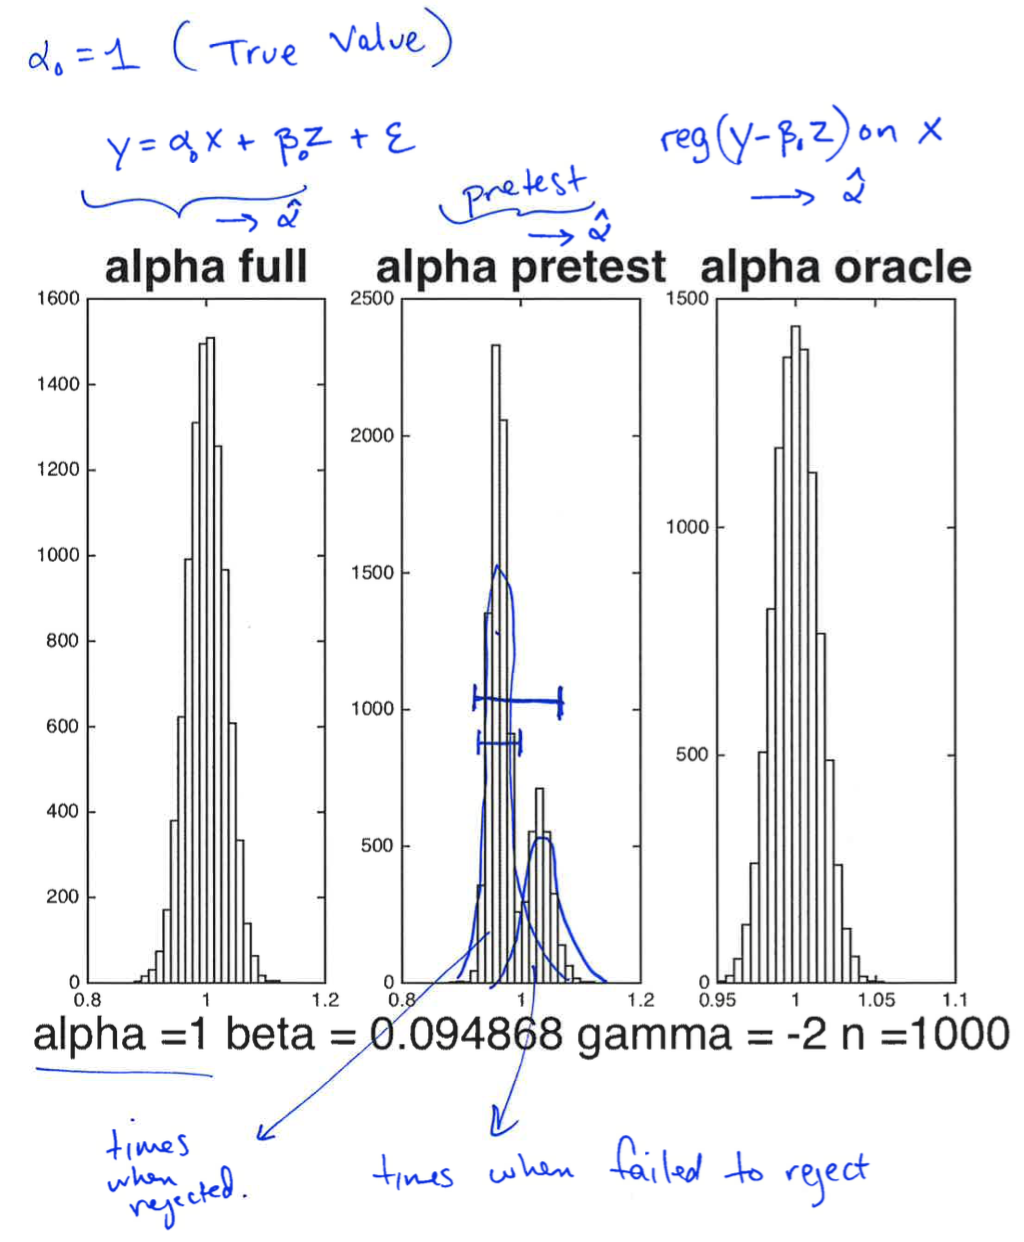
\includegraphics{figures/Fig_621.png}
\caption{Omitted Variable Bias and Pre-Test Distortion}
\end{figure}

As we can see from the figure above (code below), running the short regression instead of the long one introduces Omitted Variable Bias (second column). Instead, the Pre-Testing estimator is consistent but not normally distributed (third column).

Pre-testing is problematic because the post-selection estimator is not asymptotically normal. Moreover, for particular data generating processes, it even fails to be consistent at the rate of \(\sqrt{n}\) (Belloni et al., 2014).

\begin{quote}
Intuition: when performing pre-testing, we might have an Omitted Variable Bias problem when \(\beta_0>0\) but we fail to reject the null hypothesis \(H_0:\beta_0=0\) because of lack of statistical power, i.e.~\(|\beta_0|\) is small with respect to the sample size. In particular, we fail to reject the null hypothesis for \(\beta_0 = O\left( \frac{1}{n}\right)\). Note however, that the problem vanishes asymptotically, as the resulting estimator is consistent. In fact, if \(\beta_0(n) = O\left( \frac{1}{n}\right)\), \(\alpha_0 - \hat \alpha_{PRETEST} \overset{p}{\to} \beta_0 \gamma_0 = 0\). We now clarify what it means to have a coefficient depending on the sample size, \(\beta_0(n)\).
\end{quote}

Concept of \textbf{uniformity}: the DGP varies with \(n\). Instead of having a fixed ``true'' parameter \(\beta_0\), you have a sequence \(\beta_0(n)\).
Having a cofficient that depends on the sample size \(n\) is useful to preserve the concept of ``small with respect to the sample size'' in asymptotic theory.

In the context of Pre-Testing, all problems vanish asymptotically since we are able to always reject the null hypothesis \(H_0:\beta_0=0\) when \(\beta_0 \neq 0\). In the figure above, I plot simulation results for \(\hat \alpha_{PRETESTING}\) for a fixed coefficient \(\beta_0\) (first row) and variable coefficient \(\beta_0(n)\) that depends on the sample size (second row), for different sample sizes (columns). We see that if \(\beta_0\) is independent from the sample size (first row), the distribution of \(\hat \alpha_{PRETEST}\) is not normal in small samples and it displays the bimodality that characterizes pre-testing. However, it becomes normal in large samples. On the other hand, when \(\beta_0(n)\) depends on the sample size (second row), the distribution of \(\hat \alpha_{PRETEST}\) stays bimodal even when the sample size increases.

\begin{quote}
Note that the estimator is always consistent!
\end{quote}

\begin{figure}
\centering
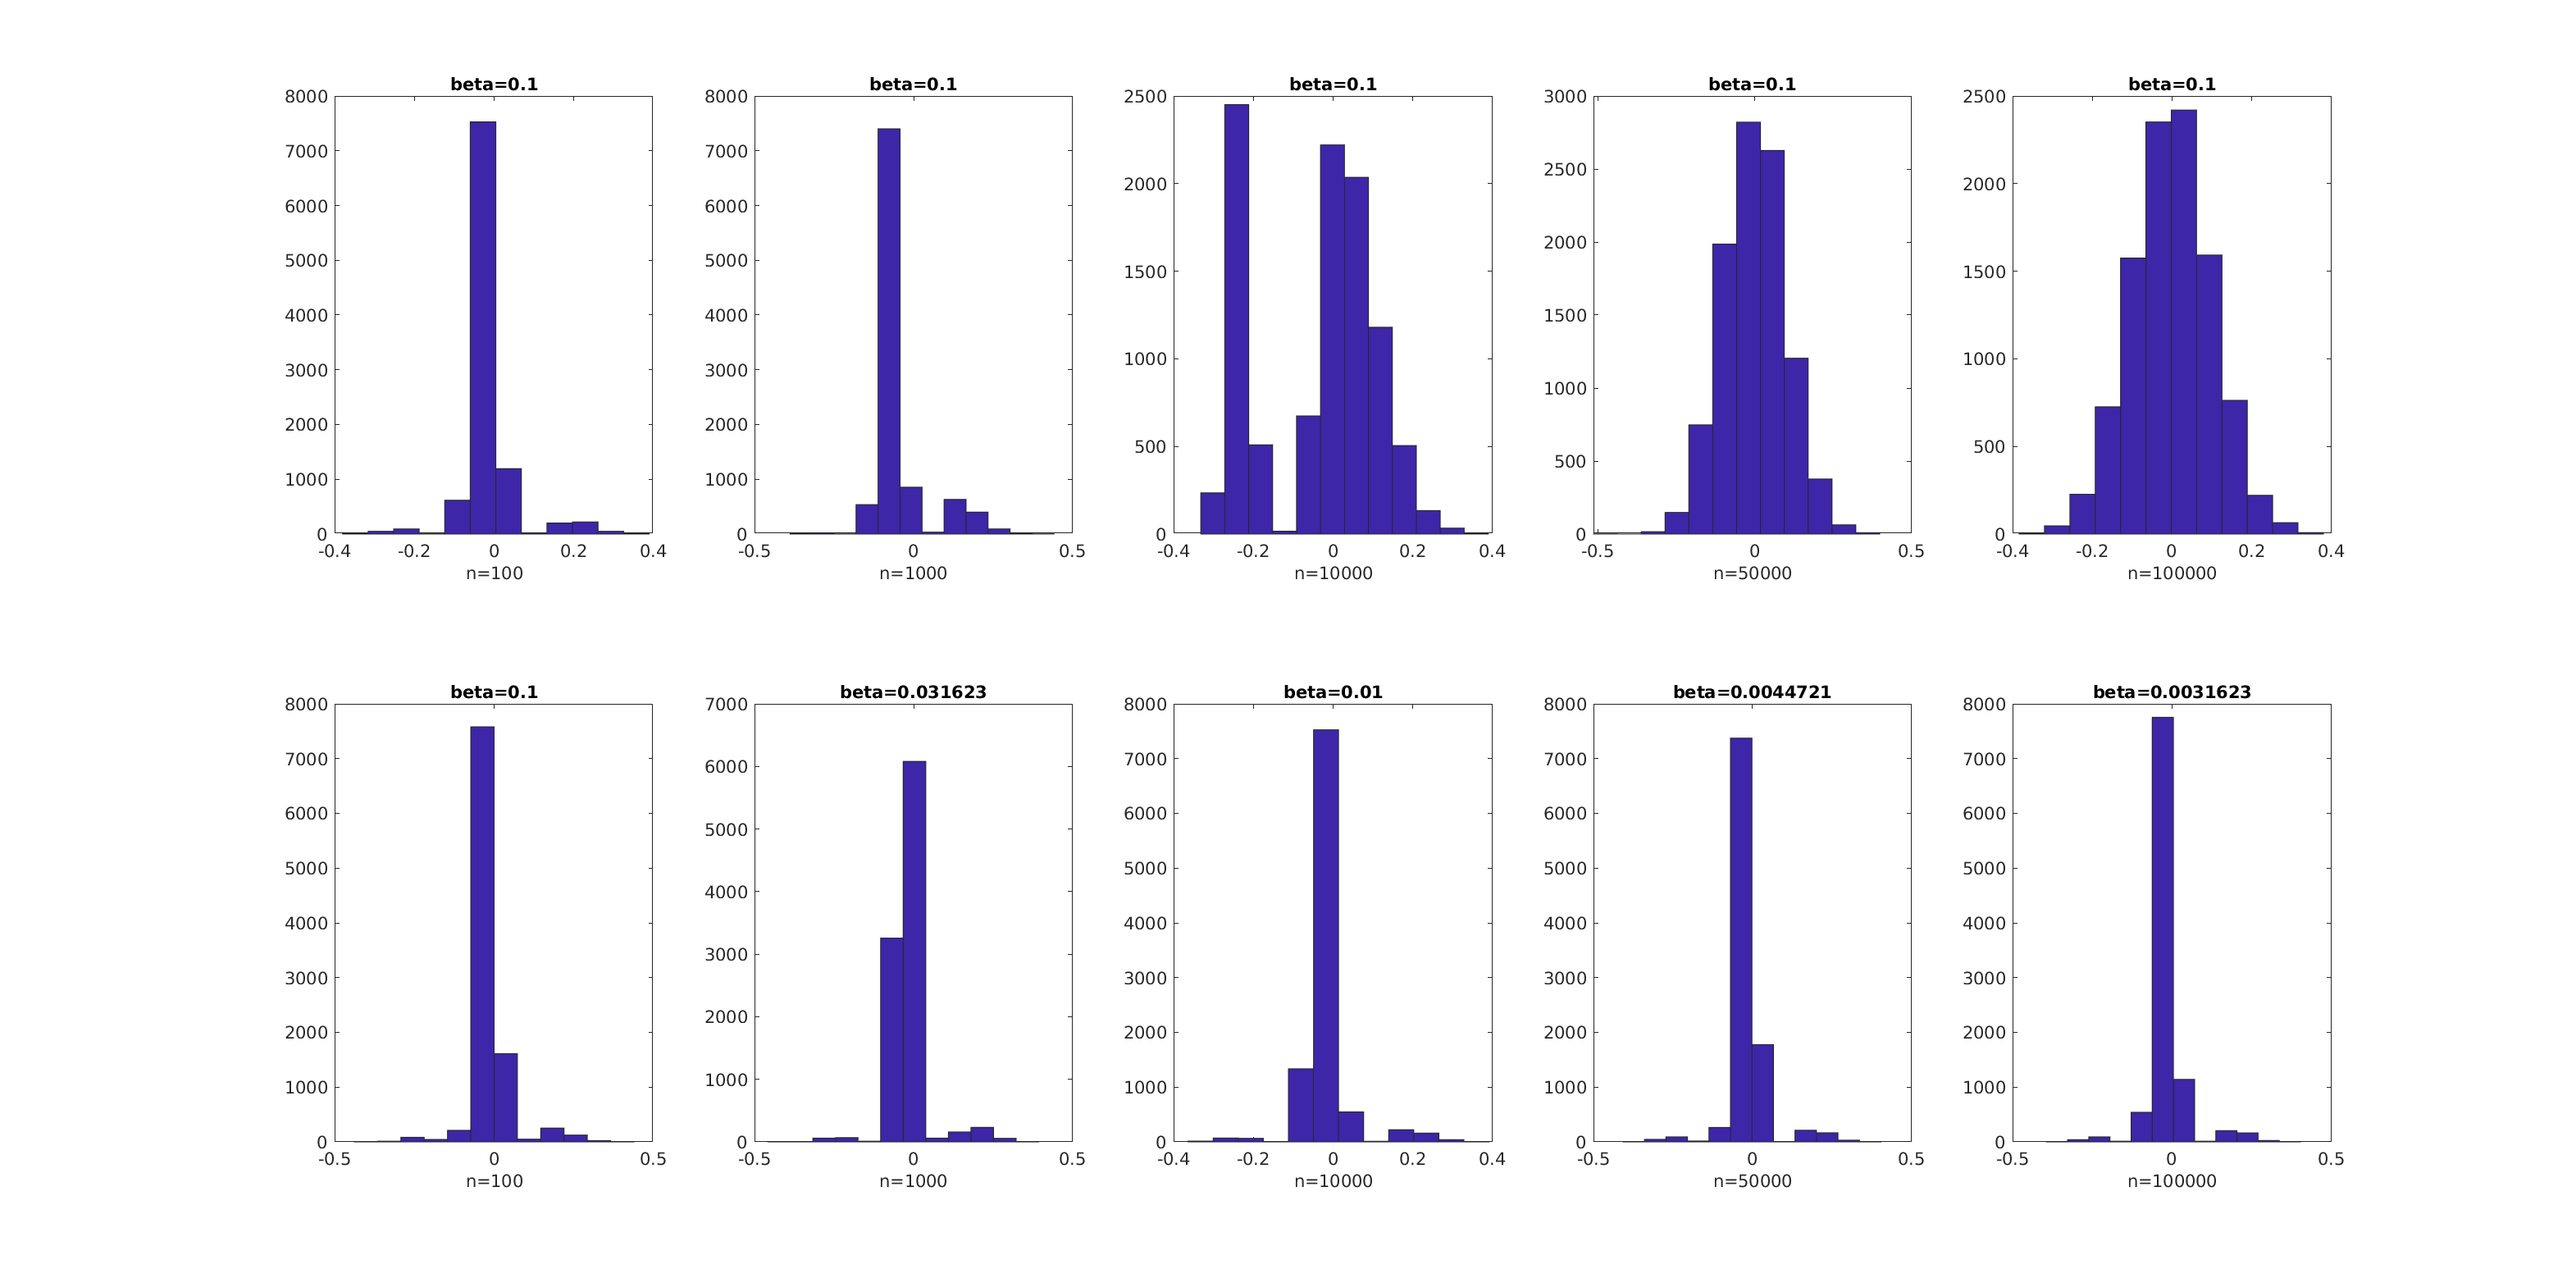
\includegraphics{figures/Fig_624.png}
\caption{Distrubution of \(\hat \alpha_{PRETEST}\)}
\end{figure}

One could show that problems arise exactly when \(\beta_0 = O\left( \frac{1}{n}\right)\). If we were to draw a map of where the gaussianity assumption of \(\beta_0(n)\) holds well, it would look like the following figure.

\begin{figure}
\centering
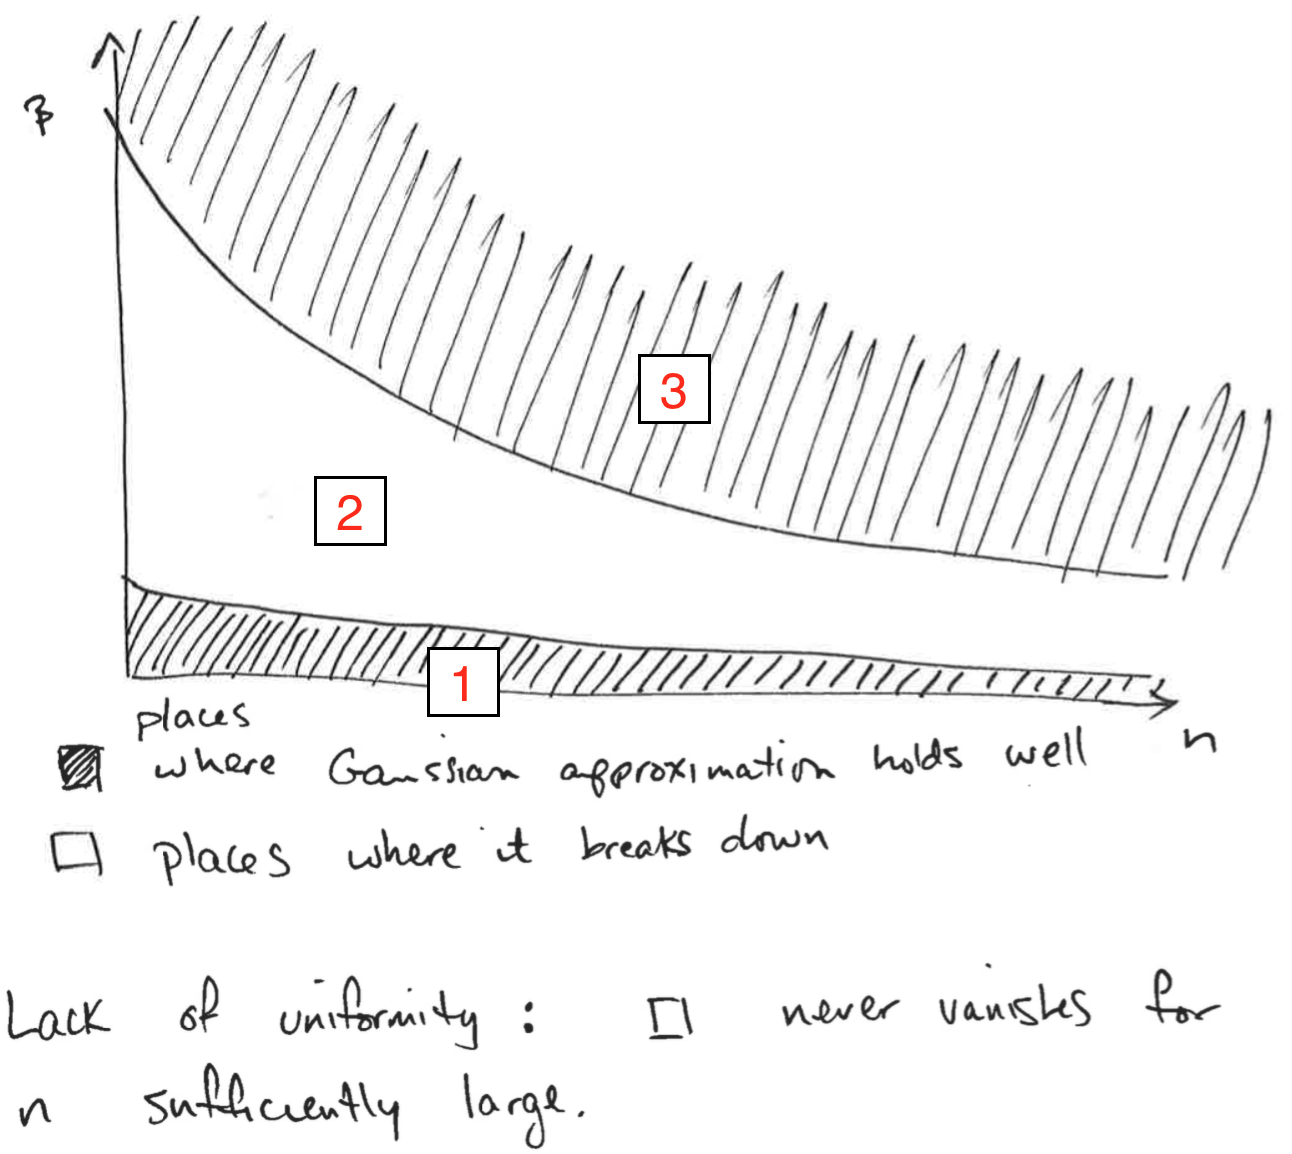
\includegraphics{figures/Fig_623.png}
\caption{Pre-test Bias}
\end{figure}

The intuition for the three different regions (from bottom to top) is the following.

\begin{enumerate}
\def\labelenumi{\arabic{enumi}.}
\tightlist
\item
  When \(\beta_0 = o(1/\sqrt{n})\), \(z_i\) is excluded with probability \(p \to 1\). But, given that \(\beta_0\) is small enough, failing to control for \(z_i\) does not introduce large omitted variables bias (Belloni et al., 2014).
\item
  If however the coefficient on the control is ``moderately close to zero'' (\(\beta_0 = O(1/\sqrt{n})\)), the t-test set-up above cannot distinguish this coefficient from \(0\), and the control \(z_i\) is dropped with probability \(p \to 1\). However, in this case the omitted variable bias generated by excluding \(z_i\) scaled by \(\sqrt{n}\) does not converge to zero. That is, the standard post-selection estimator is not asymptotically normal and even fails to be consistent at the rate of \(\sqrt{n}\) (Belloni et al., 2014).
\item
  Lastly, when \(\beta_0\) is large enough, the null pre-testing hypothesis \(H_0 : \beta_0 = 0\) will be rejected sufficiently often so that the bias is negligible.
\end{enumerate}

The post-double-selection estimator, \(\hat{\alpha}_{PDS}\) solves this problem by doing variable selection via standard t-tests or Lasso-type selectors with the two ``true model'' equations (\textbf{first stage} and \textbf{reduced form}) that contain the information from the model and then estimating \(\alpha_0\) by regressing \(y_i\) on \(x_i\) and the union of the selected controls. By doing so, \(z_i\) is omitted only if its coefficient in both equations is small which greatly limits the potential for omitted variables bias (Belloni et al., 2014).

\hypertarget{partioned-regression}{%
\subsection{Partioned Regression}\label{partioned-regression}}

\textbf{Frisch-Waugh Theorem}:
Consider the data \(D = \{ x_i, y_i, z_i \}_{i=1}^\infty\) with DGP: \(Y = X \alpha + Z \beta + \varepsilon\). The following estimators of \(\alpha\) are numerically equivalent (if \([X, Z]\) has full rank):

\begin{itemize}
\tightlist
\item
  \(\hat{\alpha}\) from regressing \(Y\) on \(X, Z\)
\item
  \(\tilde{\alpha}\) from regressing \(Y\) on \(\tilde{X}\)
\item
  \(\bar{\alpha}\) from regressing \(\tilde{Y}\) on \(\tilde{X}\)
\end{itemize}

where the operation of passing to \(Y, X\) to \(\tilde{Y}, \tilde{X}\) is called \emph{projection out \(Z\)}, e.g.\(\tilde{X}\) are the residuals from regressing \(X\) on \(Z\).

\textbf{Proof}:
We want to show that \(\hat{\alpha} = \tilde{\alpha}\).

Claim: \(\hat{\alpha } = \tilde{\alpha} \Leftrightarrow \tilde{X}' \left[ (X - \tilde{X})\hat{\alpha} + Z \hat{\beta} +\hat{\varepsilon} \right] = 0\).

Proof of the claim: if \(\hat{\alpha} = \tilde{\alpha}\), we can write \(Y\) as
\[
    Y =  X \hat{\alpha} + Z \hat{\beta} + \hat{\varepsilon}  = \tilde{X} \hat{\alpha} + \underbrace{(X - \tilde{X}) \hat{\alpha } + Z \hat{\beta} + \hat{\varepsilon}}_\text{residual of $Y$ on $\tilde{X} $} = \tilde{X} \tilde{\alpha} + \nu_i
\]

Therefore, by the orthogonality property of the OLS residual, it must be that \(\tilde{X}'\nu_i= 0\).
\[\tag*{$\blacksquare$}\]

Having established the claim, we want to show that the normal equation \(\tilde{X}' \left[ (X - \tilde{X})\hat{\alpha} + Z \hat{\beta} +\hat{\varepsilon} \right] = 0\) is satisfied. We follow 3 steps:

\begin{enumerate}
\def\labelenumi{\arabic{enumi}.}
\item
  First we have that \(\tilde{X}' (X - \tilde{X})\hat{\alpha} = 0\). This follows from the fact that \(\tilde{X}' = X' M_Z\) and hence:
  \[
    \begin{aligned}
    \tilde{X}' (X - \tilde{X})  &  = X' M_Z (X - M_Z) = X' M_Z X - X' \overbrace{M_Z M_Z}^{M_Z} X \\ & = X'M_Z X - X' M_Z X = 0
    \end{aligned}
  \]
\item
  \(\tilde{X}' Z \hat{\beta} = 0\) since \(\tilde{X}\) is the residual from the regression of \(X\) on \(Z\), by normal equation it holds that \(\tilde{X}' Z = 0\).
\item
  \(\tilde{X}' \hat{\varepsilon} = 0\). This follows from (i) \(M_Z ' M_{X, Z} = M_{X,Z}\) and (ii) \(X' M_{X, Z} = 0\):
  \[
    \tilde{X}' \hat{\varepsilon} = (M_Z X)' (M_{X, Z} \varepsilon)  = X'M_Z' M_{X, Z} \varepsilon = \underbrace{X' M_{X, Z}}_0 \varepsilon = 0.
  \]
  \[\tag*{$\blacksquare$}\]
\end{enumerate}

The coefficient \(\hat{\alpha}\) is a \emph{partial regression} coefficient identified from the variation in \(X\) that is orthogonal to \(Z\). This is often known as \textbf{residual variation}.

\hypertarget{matlab-8}{%
\subsection{\texorpdfstring{\texttt{Matlab}}{Matlab}}\label{matlab-8}}

First, we consider the following model: \$ y\_i = x\_i' \alpha\_0 + z\_i' \beta\_0 + \varepsilon\_i \$ and
\$ x\_i = z\_i' \gamma\_0 + u\_i \$ where \(\alpha_0 = 1\), \(\beta_0 = 0.1\) and \(\gamma = -4\), and \(\varepsilon_i, u_i \sim N(0,1)\). We simulate three different estimators over 10000 samples: \(\hat \alpha_{LONG}\) from the long regression, \(\hat \alpha_{SHORT}\) from the short regression and \(\hat \alpha_{PRE-TESTING}\) that is either \(\hat \alpha_{LONG}\) or \(\hat \alpha_{SHORT}\), depending on whether \(\hat \beta\) is significant at the 5\% level or not in the long regression.

\begin{Shaded}
\begin{Highlighting}[]
\CommentTok{% Set seed}
\NormalTok{rng(}\FloatTok{123}\NormalTok{)}

\CommentTok{% Define Model Parameters}
\NormalTok{n = }\FloatTok{1000}\NormalTok{;}
\NormalTok{alpha = }\FloatTok{1}\NormalTok{;}
\NormalTok{beta = }\FloatTok{.1}\NormalTok{;}
\NormalTok{gamma = -}\FloatTok{4}\NormalTok{;}

\CommentTok{% Set number of simulations}
\NormalTok{n_simulations = }\FloatTok{10000}\NormalTok{;}

\CommentTok{% Preallocate simulation results}
\NormalTok{alpha_short = zeros(n_simulations,}\FloatTok{1}\NormalTok{);}
\NormalTok{alpha_long = zeros(n_simulations,}\FloatTok{1}\NormalTok{);}
\NormalTok{alpha_pretest = zeros(n_simulations,}\FloatTok{1}\NormalTok{);}

\CommentTok{% Loop over simulations}
\NormalTok{for sim = }\FloatTok{1}\NormalTok{:n_simulations}

    \CommentTok{% Generate Data}
\NormalTok{    Z = randn(n,}\FloatTok{1}\NormalTok{);}
\NormalTok{    X = gamma*Z + randn(n,}\FloatTok{1}\NormalTok{);}
\NormalTok{    e = randn(n,}\FloatTok{1}\NormalTok{);}
\NormalTok{    Y = alpha*X+ beta*Z + e;}
    
    \CommentTok{% Alpha estimate from long regression}
\NormalTok{    alpha_short(sim) = inv(X'*X)*X'*Y;}
    
    \CommentTok{% Alpha estimate from long regression}
\NormalTok{    estimates_temp = inv([X,Z]'*[X,Z])*[X,Z]'*Y;}
\NormalTok{    alpha_long(sim) = estimates_temp(}\FloatTok{1}\NormalTok{);}

    \CommentTok{% Compute test statistic}
\NormalTok{    e = Y - [X,Z]*estimates_temp;}
\NormalTok{    t = estimates_temp(}\FloatTok{2}\NormalTok{)/sqrt(var(e)*([}\FloatTok{0}\NormalTok{,}\FloatTok{1}\NormalTok{]*inv([X,Z]'*[X,Z])*[}\FloatTok{0}\NormalTok{;}\FloatTok{1}\NormalTok{]));}
    
    \CommentTok{% Pick estimate depending on test statistic}
\NormalTok{    if abs(t)>}\FloatTok{1.96}
\NormalTok{        alpha_pretest(sim) = alpha_long(sim);}
\NormalTok{    else}
\NormalTok{        alpha_pretest(sim) = alpha_short(sim);}
\NormalTok{    end}
\NormalTok{end}

\CommentTok{% Plot results}
\NormalTok{figure}
\NormalTok{set(gcf,}\StringTok{'position'}\NormalTok{,[}\FloatTok{0}\NormalTok{,}\FloatTok{0}\NormalTok{,}\FloatTok{1000}\NormalTok{,}\FloatTok{500}\NormalTok{])}
\NormalTok{subplot(}\FloatTok{1}\NormalTok{,}\FloatTok{3}\NormalTok{,}\FloatTok{1}\NormalTok{)}
\NormalTok{hist(alpha_short, }\FloatTok{20}\NormalTok{), title([}\StringTok{'alpha short'}\NormalTok{],}\StringTok{'fontsize'}\NormalTok{,}\FloatTok{12}\NormalTok{)}
\NormalTok{subplot(}\FloatTok{1}\NormalTok{,}\FloatTok{3}\NormalTok{,}\FloatTok{2}\NormalTok{)}
\NormalTok{hist(alpha_long, }\FloatTok{20}\NormalTok{), title([}\StringTok{'alpha long'}\NormalTok{],}\StringTok{'fontsize'}\NormalTok{,}\FloatTok{12}\NormalTok{)}
\NormalTok{xlabel([}\StringTok{'alpha='}\NormalTok{,num2str(alpha),}\StringTok{', beta='}\NormalTok{,num2str(beta),}\StringTok{', gamma='}\NormalTok{,num2str(gamma),}\StringTok{', n='}\NormalTok{,num2str(n)], }\StringTok{'fontsize'}\NormalTok{,}\FloatTok{10}\NormalTok{)}
\NormalTok{subplot(}\FloatTok{1}\NormalTok{,}\FloatTok{3}\NormalTok{,}\FloatTok{3}\NormalTok{)}
\NormalTok{hist(alpha_pretest, }\FloatTok{20}\NormalTok{), title([}\StringTok{'alpha pre-test'}\NormalTok{],}\StringTok{'fontsize'}\NormalTok{,}\FloatTok{12}\NormalTok{)}
\end{Highlighting}
\end{Shaded}

Now we repeat the same exercise but for two different specifications of \(beta_0\): one that depends on the sample size \(n\) and one that does not. We check what happens for different sample sizes.

\begin{Shaded}
\begin{Highlighting}[]

\CommentTok{% Sequence of sample sizes}
\NormalTok{n_sequence = [}\FloatTok{100}\NormalTok{,}\FloatTok{1000}\NormalTok{,}\FloatTok{10000}\NormalTok{,}\FloatTok{50000}\NormalTok{,}\FloatTok{100000}\NormalTok{];}

\CommentTok{% Initialize figure}
\NormalTok{figure}
\NormalTok{set(gcf,}\StringTok{'position'}\NormalTok{,[}\FloatTok{0}\NormalTok{,}\FloatTok{0}\NormalTok{,}\FloatTok{2000}\NormalTok{,}\FloatTok{1000}\NormalTok{])}
\NormalTok{n_fig = }\FloatTok{1}\NormalTok{;}

\CommentTok{% Loop over data generating processes}
\NormalTok{for dgp=}\FloatTok{0}\NormalTok{:}\FloatTok{1}
\NormalTok{    for n=n_sequence}
\NormalTok{        for sim=}\FloatTok{1}\NormalTok{:n_simulations}

            \CommentTok{% Select beta according to dgp}
\NormalTok{            if dgp==}\FloatTok{0}
\NormalTok{                beta_n = beta;}
\NormalTok{            else}
\NormalTok{                beta_n = beta/sqrt(n)*sqrt(}\FloatTok{100}\NormalTok{);}
\NormalTok{            end}

            \CommentTok{% Generate Data}
\NormalTok{            Z = randn(n,}\FloatTok{1}\NormalTok{);}
\NormalTok{            X = gamma*Z + randn(n,}\FloatTok{1}\NormalTok{);}
\NormalTok{            e = randn(n,}\FloatTok{1}\NormalTok{);}
\NormalTok{            Y = alpha*X+ beta_n*Z + e;}

            \CommentTok{% Alpha estimate from long regression}
\NormalTok{            alpha_short(sim) = inv(X'*X)*X'*Y;}

            \CommentTok{% Alpha estimate from long regression}
\NormalTok{            estimates_temp = inv([X,Z]'*[X,Z])*[X,Z]'*Y;}
\NormalTok{            alpha_long(sim) = estimates_temp(}\FloatTok{1}\NormalTok{);}

            \CommentTok{% Compute test statistic}
\NormalTok{            e = Y - [X,Z]*estimates_temp;}
\NormalTok{            t = estimates_temp(}\FloatTok{2}\NormalTok{)/sqrt(var(e)*([}\FloatTok{0}\NormalTok{,}\FloatTok{1}\NormalTok{]*inv([X,Z]'*[X,Z])*[}\FloatTok{0}\NormalTok{;}\FloatTok{1}\NormalTok{]));}

            \CommentTok{% Pick estimate depending on test statistic}
\NormalTok{            if abs(t)>}\FloatTok{1.96}
\NormalTok{                alpha_pretest(sim) = alpha_long(sim);}
\NormalTok{            else}
\NormalTok{                alpha_pretest(sim) = alpha_short(sim);}
\NormalTok{            end}
\NormalTok{        end}

        \CommentTok{% Add subplot}
\NormalTok{        subplot(}\FloatTok{2}\NormalTok{,length(n_sequence),n_fig)}
\NormalTok{        hist((alpha_pretest-alpha)*sqrt(n/}\FloatTok{100}\NormalTok{), }\FloatTok{12}\NormalTok{)}
\NormalTok{        title([}\StringTok{'beta='}\NormalTok{,num2str(beta_n)],}\StringTok{'fontsize'}\NormalTok{,}\FloatTok{10}\NormalTok{)}
\NormalTok{        xlabel([}\StringTok{'n='}\NormalTok{,num2str(n)], }\StringTok{'fontsize'}\NormalTok{,}\FloatTok{10}\NormalTok{)}
\NormalTok{        n_fig = n_fig+}\FloatTok{1}\NormalTok{;}

\NormalTok{    end}
\NormalTok{end}
\end{Highlighting}
\end{Shaded}

\hypertarget{post-double-selection}{%
\section{Post Double Selection}\label{post-double-selection}}

Consider again data \(D= (y_i, x_i, z_i)_{i=1}^n\), where the true model is:
\[
\begin{aligned}
& y_i = x_i' \alpha_0  + z_i' \beta_0 + \varepsilon_i \\
& x_i = z_i' \gamma_0 + u_i
\end{aligned}
\]

We would like to guard against pretest bias if possible, in order to handle high dimensional models. A good pathway towards motivating procedures which guard against pretest bias is a discussion of classical partitioned regression.

Consider a regression \(y_i\) on \(x_i\) and \(z_i\). \(x_i\) is the 1-dimensional variable of interest, \(z_i\) is a high-dimensional set of control variables. We have the following procedure:

\begin{enumerate}
\def\labelenumi{\arabic{enumi}.}
\tightlist
\item
  \textbf{First Stage} selection: lasso \(x_i\) on \(z_i\). Let the selected variables be collected in the set \(S_{FS} \subseteq z_i\)
\item
  \textbf{Reduced Form} selection: lasso \(y_i\) on \(z_i\). Let the selected variables be collected in the set \(S_{RF} \subseteq z_i\)
\item
  Regress \(y_i\) on \(x_i\) and \(S_{FS} \cup S_{RF}\)
\end{enumerate}

\textbf{Theorem}:
Let \(\{P^n\}\) be a sequence of data-generating processes for \(D_n = (y_i, x_i, z_i)^n_{i=1} \in (\mathbb R \times \mathbb R \times \mathbb R^p) ^n\) where \(p\) depends on \(n\). For each \(n\), the data are iid with \(yi = x_i'\alpha_0^{(n)} + z_i' \beta_0^{(n)} + \varepsilon_i\) and \(x_i = z_i' \gamma_0^{(n)} + u_i\) where \(\mathbb E[\varepsilon_i | x_i,z_i] = 0\) and \(\mathbb E[u_i|z_i] = 0\). The sparsity of the vectors \(\beta_0^{(n)}\), \(\gamma_0^{(n)}\) is controlled by \(|| \beta_0^{(n)} ||_0 \leq s\) with \(s^2 (\log p)^2/n \to 0\). Suppose that additional regularity conditions on the model selection procedures and moments of the random variables \(y_i\) , \(x_i\) , \(z_i\) as documented in Belloni et al.~(2014). Then the confidence intervals, CI, from the post double selection procedure are uniformly valid. That is, for any confidence level \(\xi \in (0, 1)\)
\[
        \Pr(\alpha_0 \in CI) \to 1- \xi
\]

In order to have valid confidence intervals you want their bias to be negligibly. Since
\[
  CI = \left[ \hat{\alpha} \pm \frac{1.96 \cdot \hat{\sigma}}{\sqrt{n}} \right]
\]

If the bias is \(o(n^{-1/2})\) then there is no problem since it is asymptotically negligible w.r.t. the magnitude of the confidence interval. If however the the bias is \(O(n^{-1/2})\) then it has the same magnitude of the confidence interval and it does not asymptotically vanish.

The idea of the proof is to use partitioned regression. An alternative way to think about the argument is: bound the omitted variables bias. Omitted variable bias comes from the product of 2 quantities related to the omitted variable:

\begin{enumerate}
\def\labelenumi{\arabic{enumi}.}
\tightlist
\item
  Its partial correlation with the outcome, and
\item
  Its partial correlation with the variable of interest.
\end{enumerate}

If both those partial correlations are \(O( \sqrt{\log p/n})\), then the omitted variables bias is \((s \times O( \sqrt{\log p/n})^2 = o(n^{-1/2})\), provided \(s^2 (\log p)^2/n \to 0\). Relative to the \(n^{-1/2}\) convergence rate, the omitted variables bias is negligible.

In our omitted variable bias case, we want \(| \beta_0 \gamma_0 | = o \left(\frac{1}{\sqrt{n}}\right)\). Post-double selection guarantees that

\begin{itemize}
\tightlist
\item
  \emph{Reduced form} selection (pre-testing): any ``missing'' variable has \(|\beta_{0j}| \leq \frac{c}{\sqrt{n}}\)
\item
  \emph{First stage} selection (additional): any ``missing'' variable has \(|\gamma_{0j}| \leq \frac{c}{\sqrt{n}}\)
\end{itemize}

As a consequence, as long as the number of omitted variables is finite, the omitted variable bias is
\[
    OVB(\alpha) = |\beta_{0j}| \cdot|\gamma_{0j}| \leq \frac{c}{\sqrt{n}} \cdot \frac{c}{\sqrt{n}} = \frac{c^2}{n} = o \left(\frac{1}{\sqrt{n}}\right)
\]

\begin{figure}
\centering
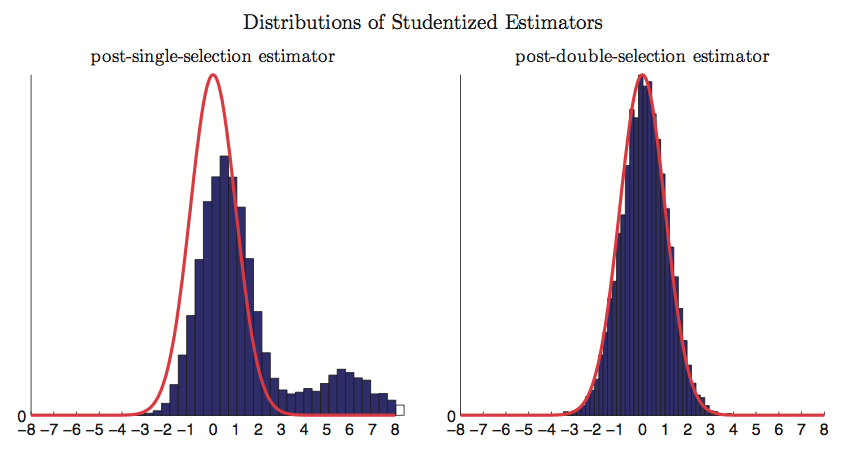
\includegraphics{figures/Fig_641.png}
\caption{Pre-test Bias}
\end{figure}

Under homoskedasticity, the above estimator achieves the semiparametric efficiency bound.

\hypertarget{references-8}{%
\section{References}\label{references-8}}

\begin{itemize}
\tightlist
\item
  Belloni, A., Chernozhukov, V., \& Hansen, C. (2014). \emph{Inference on Treatment Effects after Selection among High-Dimensional Controls}. The Review of Economic Studies, 81(2), 608--650.
\item
  Hastie, Tibshirani, Friedman (2001). ``\emph{The Elements of Statistical Learning}''.
\item
  Hansen (2019). ``\emph{Econometrics}''. Chapter 24.
\item
  Kozbur (2019). PhD Econometrics - Lecture Notes.
\end{itemize}

\hypertarget{matlabcode}{%
\chapter{Matlab Code}\label{matlabcode}}

In this appendix I collect all the matlab code from the lecture notes.

\hypertarget{lecture-1}{%
\section{Lecture 1}\label{lecture-1}}

\begin{Shaded}
\begin{Highlighting}[]
\CommentTok{% Set seed}
\NormalTok{rng(}\FloatTok{123}\NormalTok{)}

\CommentTok{% Set the number of observations}
\NormalTok{n = }\FloatTok{100}\NormalTok{;}

\CommentTok{% Set the dimension of X}
\NormalTok{k = }\FloatTok{2}\NormalTok{;}

\CommentTok{% Draw a sample of explanatory variables}
\NormalTok{X = rand(n, k);}

\CommentTok{% Draw the error term}
\NormalTok{sigma = }\FloatTok{1}\NormalTok{;}
\NormalTok{e = randn(n,}\FloatTok{1}\NormalTok{)*sqrt(sigma);}

\CommentTok{% Set the parameters}
\NormalTok{b = [}\FloatTok{2}\NormalTok{; -}\FloatTok{1}\NormalTok{];}

\CommentTok{% Calculate the dependent variable}
\NormalTok{y = X*b + e;}

\CommentTok{% Estimate beta}
\NormalTok{b_hat = inv(X'*X)*(X'*y) }\CommentTok{% = 1.9020, -0.9305}

\CommentTok{% Equivalent but faster formulation}
\NormalTok{b_hat = (X'*X)\textbackslash{}(X'*y);}

\CommentTok{% Even faster (but less intuitive) formulation}
\NormalTok{b_hat = X\textbackslash{}y;}

\CommentTok{% Note that is generally not equivalent to Var(X)^-1 * Cov(X,y)...}
\NormalTok{Var_X = cov(X);}
\NormalTok{Cov_Xy = n/(n-}\FloatTok{1}\NormalTok{) * (mean(X .* y) - mean(X).*mean(y));}
\NormalTok{b_alternative = inv(Var_X) * Cov_Xy' }\CommentTok{% = 2.1525, -0.7384}

\CommentTok{% ...unless you include a constant}
\NormalTok{a = }\FloatTok{3}\NormalTok{;}
\NormalTok{y = a + X*b + e;}
\NormalTok{b_hat_1 = [ones(n,}\FloatTok{1}\NormalTok{), X]\textbackslash{}y }\CommentTok{% = 2.1525, -0.7384}
\NormalTok{Var_X = cov(X);}
\NormalTok{Cov_Xy = n/(n-}\FloatTok{1}\NormalTok{) * (mean(X .* y) - mean(X).*mean(y));}
\NormalTok{b_alternative = inv(Var_X) * Cov_Xy' }\CommentTok{% = 2.1525, -0.7384}

\CommentTok{% Predicted y}
\NormalTok{y_hat = X*b_hat;}

\CommentTok{% Residuals}
\NormalTok{e_hat = y - X*b_hat;}

\CommentTok{% Projection matrix}
\NormalTok{P = X*inv(X'*X)*X';}

\CommentTok{% Annihilator matrix}
\NormalTok{M = eye(n) - P;}

\CommentTok{% Leverage}
\NormalTok{h = diag(P);}

\CommentTok{% Biased variance estimator }
\NormalTok{sigma_hat = e_hat'*e_hat / n;}

\CommentTok{% Unbiased estimator 1}
\NormalTok{sigma_hat_2 = e_hat'*e_hat / (n-k);}

\CommentTok{% Unbiased estimator 2}
\NormalTok{sigma_hat_3 = mean( e_hat.^}\FloatTok{2}\NormalTok{ ./ (}\FloatTok{1}\NormalTok{-h) );}

\CommentTok{% R squared - uncentered}
\NormalTok{R2_uc = (y_hat'*y_hat)/ (y'*y);}

\CommentTok{% R squared}
\NormalTok{y_bar = mean(y);}
\NormalTok{R2 = ((y_hat-y_bar)'*(y_hat-y_bar))/ ((y-y_bar)'*(y-y_bar));}

\CommentTok{% Ideal variance of the OLS estimator}
\NormalTok{var_b = sigma*inv(X'*X);}

\CommentTok{% Standard errors}
\NormalTok{std_b = sqrt(diag(var_b));}
\end{Highlighting}
\end{Shaded}

\hypertarget{lecture-2}{%
\section{Lecture 2}\label{lecture-2}}

\begin{Shaded}
\begin{Highlighting}[]
\CommentTok{% Set seed}
\NormalTok{rng(}\FloatTok{123}\NormalTok{)}

\CommentTok{% Homoskedastic standard errors}
\NormalTok{std_h = var(e_hat) * inv(X'*X);}

\CommentTok{% HC0 variance and standard errors}
\NormalTok{omega_hc0 = X' * diag(e_hat.^}\FloatTok{2}\NormalTok{) * X;}
\NormalTok{std_hc0 = sqrt(diag(inv(X'*X) * omega_hc0 * inv(X'*X))) }\CommentTok{% = 0.9195, 0.8631}

\CommentTok{% HC1 variance and standard errors}
\NormalTok{omega_hc1 = n/(n-k) * X' *  diag(e_hat.^}\FloatTok{2}\NormalTok{) * X;}
\NormalTok{std_hc1 = sqrt(diag(inv(X'*X) * omega_hc1 * inv(X'*X))) }\CommentTok{% = 0.9289, 0.8719}

\CommentTok{% HC2 variance and standard errors}
\NormalTok{omega_hc2 = X' * diag(e_hat.^}\FloatTok{2}\NormalTok{./(}\FloatTok{1}\NormalTok{-h)) * X;}
\NormalTok{std_hc2 = sqrt(diag(inv(X'*X) * omega_hc2 * inv(X'*X))) }\CommentTok{% = 0.9348, 0.8768}

\CommentTok{% HC3 variance and standard errors}
\NormalTok{omega_hc3 = X' * diag(e_hat.^}\FloatTok{2}\NormalTok{./(}\FloatTok{1}\NormalTok{-h).^}\FloatTok{2}\NormalTok{) * X;}
\NormalTok{std_hc3 = sqrt(diag(inv(X'*X) * omega_hc3 * inv(X'*X))) }\CommentTok{% = 0.9504, 0.8907}

\CommentTok{% Note what happens if you allow for full autocorrelation}
\NormalTok{omega_full = X'*e_hat*e_hat'*X;}

\CommentTok{% t-test for beta=0}
\NormalTok{t = abs(b_hat./(std_hc1));}

\CommentTok{% p-value}
\NormalTok{p_val = }\FloatTok{1}\NormalTok{ - normcdf(t);}

\CommentTok{% F statistic of joint significance}
\NormalTok{SSR_u = e_hat'*e_hat;}
\NormalTok{SSR_r = y'*y;}
\NormalTok{F = (SSR_r - SSR_u)/k / (SSR_u/(n-k));}

\CommentTok{% 95% confidente intervals}
\NormalTok{conf_int = [b_hat - }\FloatTok{1.96}\NormalTok{*std_hc1, b_hat + }\FloatTok{1.96}\NormalTok{*std_hc1];}
\end{Highlighting}
\end{Shaded}

\hypertarget{lecture-3}{%
\section{Lecture 3}\label{lecture-3}}

\begin{Shaded}
\begin{Highlighting}[]
\CommentTok{% Set seed}
\NormalTok{rng(}\FloatTok{123}\NormalTok{)}

\CommentTok{% Set the dimension of Z}
\NormalTok{l = }\FloatTok{3}\NormalTok{;}

\CommentTok{% Draw instruments}
\NormalTok{Z = randn(n,l);}

\CommentTok{% Correlation matrix for error terms}
\NormalTok{S = eye(}\FloatTok{2}\NormalTok{,}\FloatTok{2}\NormalTok{); S(}\FloatTok{1}\NormalTok{,}\FloatTok{2}\NormalTok{)=}\FloatTok{.8}\NormalTok{; S(}\FloatTok{2}\NormalTok{,}\FloatTok{1}\NormalTok{)=}\FloatTok{.8}\NormalTok{; }

\CommentTok{% Endogenous X}
\NormalTok{gamma = [}\FloatTok{2}\NormalTok{, }\FloatTok{0}\NormalTok{; }\FloatTok{0}\NormalTok{, -}\FloatTok{1}\NormalTok{; -}\FloatTok{1}\NormalTok{, }\FloatTok{3}\NormalTok{];}
\NormalTok{e = randn(n,}\FloatTok{2}\NormalTok{)*chol(S);}
\NormalTok{X = Z*gamma + e(:,}\FloatTok{1}\NormalTok{);}

\CommentTok{% Calculate Y}
\NormalTok{Y = X*b + e(:,}\FloatTok{2}\NormalTok{);}

\CommentTok{% Estimate beta OLS}
\NormalTok{beta_OLS = (X'*X)\textbackslash{}(X'*Y) }\CommentTok{% = 2.1957, -0.9022}

\CommentTok{% IV: l=k=2 instruments}
\NormalTok{Z_IV = Z(:,}\FloatTok{1}\NormalTok{:k);}
\NormalTok{beta_IV = (Z_IV'*X)\textbackslash{}(Z_IV'*Y) }\CommentTok{% = 2.1207, -1.3617}

\CommentTok{% Calculate standard errors}
\NormalTok{ehat = Y - X*beta_IV;}
\NormalTok{V_NHC_IV = var(ehat) * inv(Z_IV'*X)*Z_IV'*Z_IV*inv(Z_IV'*X);}
\NormalTok{V_HC0_IV = inv(Z_IV'*X)*Z_IV' * diag(ehat.^}\FloatTok{2}\NormalTok{) * Z_IV*inv(Z_IV'*X);}

\CommentTok{% 2SLS: l=3 instruments}
\NormalTok{Pz = Z*inv(Z'*Z)*Z';}
\NormalTok{beta_2SLS = (X'*Pz*X)\textbackslash{}(X'*Pz*Y) }\CommentTok{% = 2.0723, -0.9628}

\CommentTok{% Calculate standard errors}
\NormalTok{ehat = Y - X*beta_2SLS;}
\NormalTok{V_NCH_2SLS = var(ehat) * inv(X'*Pz*X);}
\NormalTok{V_HC0_2SLS = inv(X'*Pz*X)*X'*Pz * diag(ehat.^}\FloatTok{2}\NormalTok{) *Pz*X*inv(X'*Pz*X);}

\CommentTok{% GMM 1-step: inefficient weighting matrix}
\NormalTok{W_1 = eye(l);}

\CommentTok{% Objective function}
\NormalTok{gmm_1 = @(b) ( Y - X*b )' * Z * W_1 *  Z' * ( Y - X*b );}

\CommentTok{% Estimate GMM}
\NormalTok{beta_gmm_1 = fminsearch(gmm_1, beta_OLS) }\CommentTok{% = 2.0763, -0.9548}
\NormalTok{ehat = Y - X*beta_gmm_1;}

\CommentTok{% Standard errors GMM}
\NormalTok{S_hat = Z'*diag(ehat.^}\FloatTok{2}\NormalTok{)*Z;}
\NormalTok{d_hat = -X'*Z;}
\NormalTok{V_gmm_1 = inv(d_hat * inv(S_hat) * d_hat');}

\CommentTok{% GMM 2-step: efficient weighting matrix}
\NormalTok{W_2 = inv(S_hat);}
\NormalTok{gmm_2 = @(b) ( Y - X*b )' * Z * W_2 *  Z' * ( Y - X*b );}
\NormalTok{beta_gmm_2 = fminsearch(gmm_2, beta_OLS) }\CommentTok{% = 2.0595, -0.9666}

\CommentTok{% Standard errors GMM}
\NormalTok{ehat = Y - X*beta_gmm_2;}
\NormalTok{S_hat = Z'*diag(ehat.^}\FloatTok{2}\NormalTok{)*Z;}
\NormalTok{d_hat = -X'*Z;}
\NormalTok{V_gmm_2 = inv(d_hat * inv(S_hat) * d_hat');}
\end{Highlighting}
\end{Shaded}

\newpage


\end{document}
